\documentclass[10pt,a4paper,twocolumn]{article}

\usepackage[T1]{fontenc}
\usepackage[utf8]{inputenc}
\usepackage{mathptmx}                 % Times-like serif body
% Times pour tout le document : titres compris (pas de sans-serif)
\usepackage[left=20mm,right=20mm,top=24mm,bottom=24mm,
            columnsep=7mm]{geometry}
\usepackage{amsmath,amssymb,bm}
\usepackage{siunitx}
\usepackage{graphicx}
\usepackage{booktabs,threeparttable}
\usepackage[font=small,labelfont=bf,labelsep=period,
            justification=centering]{caption}
\usepackage{enumitem}
\usepackage[explicit]{titlesec}
\usepackage{stfloats}
\usepackage{flafter}
\setcounter{topnumber}{3}
\setcounter{bottomnumber}{2}
\setcounter{totalnumber}{4}
\setcounter{dbltopnumber}{2}
\renewcommand{\topfraction}{0.92}
\renewcommand{\bottomfraction}{0.6}
\renewcommand{\floatpagefraction}{0.88}
\usepackage[hidelinks]{hyperref}
\usepackage[numbers,sort&compress]{natbib}
\usepackage{doi}          % prints the DOI of every reference that has one

\titleformat{\section}{\rmfamily\bfseries\fontsize{11.5}{14}\selectfont}{\thesection.}{0.7em}{#1}
\titleformat{\subsection}{\rmfamily\bfseries\fontsize{10.5}{12.5}\selectfont}{\thesubsection.}{0.6em}{#1}
\titleformat{\subsubsection}{\rmfamily\itshape\fontsize{9.5}{11.5}\selectfont}{\thesubsubsection.}{0.5em}{#1}
\titlespacing*{\section}{0pt}{11pt plus 3pt minus 2pt}{5pt plus 1pt}
\titlespacing*{\subsection}{0pt}{8pt plus 2pt minus 1pt}{3pt plus 1pt}
\titlespacing*{\subsubsection}{0pt}{7pt plus 2pt minus 1pt}{2.5pt}
% Le point final est porte par le titre et non par le compteur : sans cela
% \ref produit << Section 5.2.. >> en fin de phrase.
\renewcommand{\thesection}{\arabic{section}}
\renewcommand{\thesubsection}{\arabic{section}.\arabic{subsection}}
\renewcommand{\thesubsubsection}%
  {\arabic{section}.\arabic{subsection}.\arabic{subsubsection}}
\setlength{\abovecaptionskip}{4pt}
\setlength{\belowcaptionskip}{2pt}
\setlength{\parindent}{0pt}
\setlength{\abovedisplayskip}{5.5pt plus 1.5pt minus 1pt}
\setlength{\belowdisplayskip}{5.5pt plus 1.5pt minus 1pt}
\setlength{\abovedisplayshortskip}{3pt plus 1pt}
\setlength{\belowdisplayshortskip}{3.5pt plus 1pt}
\setlength{\jot}{3pt}
\setlength{\parskip}{3.2pt plus 1pt minus 0.5pt}
\setlength{\textfloatsep}{9pt plus 2pt minus 2pt}
\setlength{\intextsep}{8pt plus 2pt minus 2pt}
\setlength{\floatsep}{7pt plus 2pt minus 2pt}
\setlength{\dbltextfloatsep}{10pt plus 2pt minus 2pt}
\renewcommand{\dbltopfraction}{0.92}
\renewcommand{\dblfloatpagefraction}{0.92}
\renewcommand{\textfraction}{0.10}

\graphicspath{{figures/}}

\DeclareSIUnit{\ampereturn}{At}
\DeclareSIUnit{\rpm}{rpm}
\DeclareSIUnit{\pp}{p.p.}
% \textohm is absent from the T1 Times text companion and prints as a
% black box; the math glyph is used instead. Rendering only, no unit change.
\DeclareSIUnit{\ohm}{\ensuremath{\Omega}}
\sisetup{detect-all,per-mode=symbol,range-phrase={--},range-units=single}

% --- macros reprises a l'identique de MEC_DtN_paper_v2.tex -------------
\newcommand{\Rs}{R_{\mathrm{s}}}
\newcommand{\Rro}{R_{\mathrm{ro}}}
\newcommand{\rmi}{r_{\mathrm{mi}}}
\newcommand{\murec}{\mu_{\mathrm{r}}}
\newcommand{\Ua}{U_{\mathrm{a}}}
\newcommand{\Um}{U_{\mathrm{m}}}
\newcommand{\Xg}{X_{\mathrm{g}}}
\newcommand{\keywordsline}[1]{\par\noindent\textbf{Keywords}\quad #1}

% --- environnements de theoreme, requis par la section 3 ---------------
\usepackage{amsthm}
\theoremstyle{plain}
\newtheorem{proposition}{Proposition}
% Le carre de fin de demonstration (halmos) est retire a la demande de l'auteur.
\renewcommand{\qedsymbol}{}
\theoremstyle{remark}
\newtheorem{remark}{Remark}

\begin{document}

\twocolumn[
\begin{center}
{\rmfamily\bfseries\fontsize{15}{19}\selectfont
A Well-Posed Dirichlet-to-Neumann Air-Gap Operator for Magnetic
Equivalent Circuits: Trace Conformity, and Validation on a
15-Slot/14-Pole PMSM\par}
\vspace{7mm}
{\rmfamily\bfseries\fontsize{10}{13}\selectfont
Idris Laouar$^{1}$ $\cdot$ Ahcene Boukadoum$^{1}$ $\cdot$ Nabil Mezhoud$^{1}$\par}
\end{center}
\vspace{6mm}

{\rmfamily\bfseries Abstract}\par\vspace{2pt}
Magnetic equivalent circuits capture saturation and arbitrary geometry more
cheaply than finite elements, but close their air gap with an empirical
permeance function, the only element not derived from the geometry, and the
one that fixes the accuracy. We replace it by the exact Dirichlet-to-Neumann
operator of a two-layer annulus, carrying the magnetisation as a source and
condensing into a symmetric admittance matrix on a saturable reluctance
mesh. The central result concerns that condensation, not the operator: a
reluctance network holds one potential per node, so its natural bore trial
space is piecewise constant and lies outside $H^{1/2}$, the trace space on
which the operator is bounded. We prove in closed form that the self-energy
of a bore column grows as $\ln N$ without bound, and that a
piecewise-linear basis restores an absolutely convergent series. Under the
discontinuous basis the condensed operator has no limit: truncation selects
a value rather than approximating one, for any condensation of a surface
operator onto such a basis. Against two-dimensional finite elements on a
\SI{750}{\watt} 15-slot/14-pole machine, the lumped model used throughout
agrees within \SI{1.24}{\percent} on synchronous inductance,
\SI{1.11}{\percent} on flux linkage and \SI{0.28}{\percent} on the
fundamental air-gap flux density. A refined polar mesh reaches
\SI{0.10}{\percent}, \SI{0.24}{\percent} and \SI{0.31}{\percent}, the first
a cancellation of two errors of opposite sign, \SI{0.33}{\percent} against
the reference mutual inductance. Slot sidebands and cogging torque, governed
by a tooth-tip corner singularity, are reported as bounds. A five-test audit
of the finite-element reference is contributed.
\vspace{4mm}

{\rmfamily\bfseries Keywords}\quad Magnetic equivalent circuit $\cdot$ Reluctance network
$\cdot$ Dirichlet-to-Neumann operator $\cdot$ Steklov--Poincar\'e operator $\cdot$ Trace space $\cdot$ Air-gap modelling $\cdot$
Permanent-magnet machine $\cdot$ Finite-element validation
\vspace{4mm}
\vspace{5mm}

\begin{center}{\rmfamily\bfseries Nomenclature}\end{center}
\vspace{-1mm}
{\footnotesize
\parbox[t]{0.485\textwidth}{\begin{tabular}{@{}p{16mm}p{56mm}@{}}
$\varphi$ & magnetic scalar potential (A)\\
$u_{\mathrm{s}}$, $u_{\mathrm{r}}$ & bore potential, stator / rotor side\\
$\Rs$, $\Rro$, $\rmi$ & stator bore, magnet outer, magnet inner radius\\
$\Ua$, $\Um$ & logarithmic thickness of air and magnet layer\\
$\Xg$ & logarithmic thickness of a bare air annulus, $\ln(\Rs/\Rro)$\\
$g$, $L$ & mechanical air gap, active length\\
$\murec$ & magnet recoil permeability\\
$M_r$, $M_n$ & radial magnetisation, order-$n$ coefficient\\
$B_r$, $B_t$ & radial and tangential flux density\\
$p$, $N_{\mathrm{s}}$, $N_{\mathrm{m}}$ & pole pairs, stator slots, poles\\
\end{tabular}}\hfill
\parbox[t]{0.485\textwidth}{\begin{tabular}{@{}p{16mm}p{56mm}@{}}
$\nu$, $n$ & spatial order of an air-gap harmonic\\
$\alpha_n$, $\beta_n$ & transfer and magnet term at $r=\Rro$\\
$g_n$, $b_n$ & bore admittance and source, order $n$ (\si{\henry\per\metre\squared})\\
$\hat{g}_n$ & assembled bore admittance, $\pi L\Rs g_n$ (\si{\henry})\\
$\bm{Y}$ & condensed bore admittance matrix\\
$\bm{i}_{\mathrm{src}}$ & magnet source vector\\
$W_n$ & projection of the basis onto order $n$\\
$H^{1/2}$ & trace space of the annulus problem\\
$\mathcal{R}_{\mathrm{d}}$ & differential reluctance $(\ell/A)\,\mathrm{d}H/\mathrm{d}B$ (\si{\ampere\per\weber})\\
$G_{\mathrm{d}}$ & differential permeance $1/\mathcal{R}_{\mathrm{d}}$ (\si{\henry})\\
$M_{\mathrm{s}}$, $L_{\mathrm{s}}$ & angular columns, radial layers of the mesh\\
$N$, $N_h$ & harmonic truncation\\
$n_{\mathrm{sh}}$ & mesh layers per shoe sub-region\\
$k_{\mathrm{r}}$, $k_{\mathrm{l}}$ & reluctance and leakage factor\\
$\phi$, $\theta$ & rotor position, angular coordinate\\
\end{tabular}}\par}

]

\clearpage

\footnotetext[1]{Department of Electrical Engineering, Electrotechnical
Laboratory Skikda (LES), University 20 August 1955, 26 Road El Hadaiek,
21000 Skikda, Algeria. Corresponding author: Idris Laouar,
\texttt{idris.laouar@univ-skikda.dz}.}
%=======================================================================
%  NOMENCLATURE -- conservee : atout de lisibilite que les rapporteurs
%  relevent (SPEC v3 §9). Les symboles propres a la machine asynchrone
%  passent a l'Article II.
%=======================================================================
\vspace{4mm}

%=======================================================================
%  ARTICLE I -- INTRODUCTION
%  Cinq mouvements, prose continue, aucune liste (ni enumerate, ni
%  description, ni \paragraph).  Version courte : les six contributions
%  numerotees C1--C6 passent en prose, la taxonomie des fermetures perd
%  ses etiquettes (i)--(iv), le tableau tab:position est conserve.
%
%  ANCRAGE DES CHIFFRES (7 aout 2026) :
%   - 343 V / 157 V / 2,2 % : ces trois valeurs n'existaient QUE dans
%     l'introduction, sans aucun ancrage dans le corps ni dans un .txt.
%     Retirees.  L'argument du levier est desormais porte par
%     l'enveloppe terminale 468 V sur bus 500 V, tab:sweep, ligne
%     1159 tr/min, colonne FEA -- valeur publiee dans le corps.
%   - tous les autres chiffres verifies present dans le corps a la meme
%     valeur (audit programmatique).
%
%  CITATIONS :
%   - zarko2008 etait declare dans le .bib et cite nulle part ; c'est la
%     solution du couple de detente par transformation conforme, donc a
%     sa place aux cotes de zarko2006b dans la famille (ii).
%   - abdelrazek1982 = ELEMENT D'ENTREFER (art anterieur le plus proche),
%     et non methode sous-domaine : classement conserve au §1.3.
%
%  NON-RECOUVREMENT AVEC L'ARTICLE II :
%   l'Article II resume la taxonomie en quatre lignes et renvoie ici
%   pour le detail ; le present §1.3 ne reutilise aucune de ses phrases.
%=======================================================================
\section{Introduction}
\label{sec:intro}

\subsection{Reluctance Networks and the Treatment of the Air-Gap Region}

A magnetic equivalent circuit (MEC) discretises the iron of a machine rather
than its field~\cite{ostovic1989,sudhoff,amrhein}. Every branch is drawn
from the geometry, a length, a cross-section, a measured $B(H)$
curve, so saturation is represented without approximation and an
arbitrary slot profile costs nothing, while the nodal system stays small
enough to be swept: the refined network used in this paper carries
\num{10800} unknowns. Both principal machine families have been built
this way, the cage coupled to the network on induction
machines~\cite{ostovic1986,hosseini2026} and the magnet entered as a
source branch on permanent-magnet ones~\cite{hsieh,sapmaz2022}, and the
construction is still being extended, to large
turbogenerators~\cite{zhang2022} and to traction and propulsion
drives~\cite{watthewaduge2023}.

The discretisation stops at the bore. There is no iron between the two
surfaces and therefore no path along which to lay a tube, so the
permeance of the tooth-to-tooth channels that stand in for the annulus
has to be brought in from outside the model, and it is the only quantity
in the network that is. On a surface-mounted permanent-magnet machine
that import is asked to do more than close the circuit: the region it
represents is not one medium but two, air and magnet, and it carries the
source of the machine.

\subsection{Influence of the Imported Air-Gap Permeance on Model Fidelity}
\label{sub:cost}

What follows from that single import is not confined to the accuracy of
the field. A network of radial branches produces no tangential flux
density at all, so the Maxwell stress cannot be formed from the network
and the torque must be recovered from a derivative of co-energy; the
harmonic content of the torque is then whatever the air-gap treatment
allows it to be. On the \SI{750}{\watt} machine studied here, closing
the gap with an equivalent uniform width and Carter's factor
$k_{\mathrm{C}}=1.0100$ suppresses the first slot sideband
\emph{entirely}, a smooth gap has no slot harmonic by
construction, and leaves the tangential field low by
\SI{19.7}{\percent} against the finite-element analysis (FEA) reference
(Table~\ref{tab:carter}).

\begin{table*}[!t]
\centering
\begin{threeparttable}
\footnotesize
\begin{tabular}{@{}lrrrrrr@{}}
\toprule
Closure & $\gamma_m$ & $\gamma_z$ & elem./rev
& $\nu=8$ & $\nu=22$ & $B_t$ rms\\
\midrule
N1 smooth $+$ Carter        & ---      & ---      & ---   & $-100\%$   & $-100\%$  & $-19.7\%$\\
N2 generic $\cos^2$         & ---      & ---      & ---   & $+307.1\%$ & $+144.3\%$& $-19.7\%$\\
N2b Silva, $a_r=0.25\,a_t$  & 0.135452 & 0.225754 & 69.58 & $\bm{-8.7\%}$ & $-45.2\%$ & $-19.7\%$\\
N2b Silva, $a_r=0.50\,a_t$  & 0.090301 & 0.270904 & 34.79 & $+170.1\%$ & $+62.1\%$ & $-19.7\%$\\
N2b Silva, $a_r=1.00\,a_t$  & 0.000000 & 0.361206 & 17.40 & $-96.4\%$  & $-97.8\%$ & $-19.7\%$\\
\textbf{N3 operator}        & ---      & ---      & ---   & $\bm{-8.1\%}$ & $+7.6\%$ & $\bm{+7.4\%}$\\
\midrule
FEA reference & \multicolumn{3}{l}{}
& \SI{0.01966}{\tesla} & \SI{0.03276}{\tesla} & \SI{0.1333}{\tesla}\\
\bottomrule
\end{tabular}
\begin{tablenotes}[flushleft]\footnotesize
\item PMSM 15/14, lumped iron network, linear
solver at $\mu_{\mathrm{r}}=\num{3000}$, $k_{\mathrm{f}}=\num{0.325}$.
Tooth-face arc $a_t=\SI{0.361206}{\radian}$, that is
\num{17.40} elements per revolution.
\item Every closure of the N1--N2b family returns
$B_{g1}=\SI{1.0958}{\tesla}$, \SI{+2.0}{\percent}, against
\SI{1.0775}{\tesla} for N3, \SI{+0.3}{\percent}. The mean of each
modulation is unity to six decimals, which is why the fundamental is
common to all of them.
\item Spread of the first sideband over the three N2b rows:
\SI{219}{\percent}.
\end{tablenotes}
\end{threeparttable}
\caption{Air-gap closure at fixed iron model. All rows use the same
lumped iron network, so any difference is attributable to the closure
alone. The three N2b rows differ only in the tangential discretisation
that sets $\gamma_m$ and $\gamma_z$.}
\label{tab:carter}
\end{table*}

Closures built on an identified coupling kernel escape that suppression,
but each new geometry then requires its own finite-element bench. That
inverts the purpose of a reduced-order model: a method adopted in order
to explore a design space cannot enter a region of that space without
first being calibrated there by the method it was meant to replace.

At system level the error does not even stay proportional. The machine
is fed from a \SI{500}{\volt} dc bus, and near the upper end of its
speed range the terminal envelope of the reference stands at
\SI{468}{\volt} (Table~\ref{tab:sweep}); what remains to drive the
current is a small difference between two large numbers. A relative
error on the electromotive force (EMF) therefore reappears on the current, and
on everything the current determines, magnified by the ratio of the bus
voltage to that margin. An air-gap description good to a few percent on
flux density is not, on that account, good enough for the drive-level
use for which the circuit was adopted. This lever governs the reading of
every drive result reported in Section~\ref{sub:drive} and is not
restated there.

\begin{table*}[!t]
\centering
\footnotesize
\begin{threeparttable}
\begin{tabular}{rrrrrrrrr}
\toprule
$n$ & \multicolumn{2}{c}{torque (N\,m)} & \multicolumn{2}{c}{$P_{\mathrm{em}}$ (W)}
    & \multicolumn{2}{c}{$I$ rms (A)} & \multicolumn{2}{c}{envelope (V)}\\
\cmidrule(lr){2-3}\cmidrule(lr){4-5}\cmidrule(lr){6-7}\cmidrule(lr){8-9}
(rpm) & MEC & FEA & MEC & FEA & MEC & FEA & MEC & FEA \\
\midrule
10\tnote{a}   & 30.68 & 29.23 & 32   & 31   & 19.80 & 24.35 & 11  & 1   \\
297  & 23.10 & 24.03 & 719  & 748  & 14.50 & 15.88 & 289 & 182 \\
584  & 17.47 & 20.49 & 1069 & 1254 & 9.44  & 11.95 & 458 & 325 \\
872  & 11.70 & 16.38 & 1068 & 1495 & 4.56  & 7.46  & 492 & 444 \\
1159 & 6.66  & 9.20  & 808  & 1116 & 2.05  & 3.04  & 477 & 468 \\
1446 & 2.27  & 2.96  & 344  & 449  & 0.67  & 0.90  & 487 & 482 \\
1676 & $-0.08$ & 0.09 & $-13$ & 16 & 0.03  & 0.04  & 501 & 499 \\
\bottomrule
\end{tabular}

\vspace{3mm}

\begin{tabular}{lrrr}
\toprule
Quantity & MEC & FEA & deviation \\
\midrule
stall torque (N\,m)          & 30.68 & 29.23 & $+5.0\%$ \\
no-load speed (rpm)          & 1658  & 1680  & $-1.3\%$ \\
peak power (W)               & 1115  & 1495  & $-25.4\%$ \\
\quad reached at (rpm)       & 642   & 929   &, \\
back-EMF constant $k_E$ (mV/rpm) & 312.8 & 323.6 & $-3.3\%$ \\
peak efficiency (\%)         & 85.45 & 89.43 & $-3.99$ p.p.\tnote{c} \\
\midrule
\multicolumn{4}{l}{\emph{Mean absolute deviation over the 28 points above \SI{100}{\rpm}}\tnote{d}}\\
torque, electromagnetic power & \multicolumn{3}{c}{$25.8\%$} \\
phase current                 & \multicolumn{3}{c}{$25.3\%$} \\
terminal envelope             & \multicolumn{3}{c}{$24.8\%$} \\
dc-bus current                & \multicolumn{3}{c}{$38.1\%$} \\
flux linkage, rms             & \multicolumn{3}{c}{$22.1\%$} \\
efficiency                    & \multicolumn{3}{c}{$6.1$ p.p.} \\
\textbf{torque per ampere}    & \multicolumn{3}{c}{$\bm{15.1\%}$} \\
\bottomrule
\end{tabular}
\begin{tablenotes}[flushleft]\footnotesize
\item[a] Not a periodic steady-state average in the reference; see
Test~5 of Section~\ref{sec:audit}.
\item[c] \emph{In points, per the rule of Section~\ref{sub:stats}.}
Earlier versions of this table printed \num{-4.5}, which is the
\emph{relative} deviation $85.4456/89.4319-1=\SI{-4.46}{\percent}$ formed
on the full-precision values. The two efficiencies also occur at
different speeds, so the row compares two peaks and not one operating
point.
\item[d] The sweep steps by \SI{57.44}{\rpm}, so \emph{two} of its
thirty points lie at or below \SI{100}{\rpm}, \SI{10}{\rpm} and
\SI{67.4}{\rpm}, and twenty-eight above. Only the first is listed in
the upper panel, which is why the count is stated here.
\end{tablenotes}
\end{threeparttable}
\caption{PMSM speed sweep at a \SI{500}{\volt} dc bus, thirty points from
\SI{10}{\rpm} to \SI{1676}{\rpm}. Upper panel: seven representative
points. Lower panel: the anchors of the characteristic and the mean
deviations.}
\label{tab:sweep}
\end{table*}

\subsection{Classification of Existing Air-Gap Closure Formulations}
\label{sub:positioning}

Each of the four treatments in use is limited in a way that belongs to
its construction rather than to its implementation.

An equivalent uniform gap $g_{\mathrm{eff}}=k_{\mathrm{C}}g$ restores
the mean flux and discards the rest~\cite{carter,pyrhonen}: the slot
harmonics disappear and no tangential component is produced. A permeance
modulation $\Lambda(\theta)$ superimposed on the smooth-gap solution
brings them back~\cite{zhu1993}, and in the complex form of
\v{Z}arko, Ban and Lipo it returns both field components exactly for a
slotted stator facing a smooth rotor, and yields the cogging torque
through the same conformal map~\cite{zarko2006b,zarko2008}; but the
modulation is derived in a linear medium and superposed on the magnet
solution, so saturation is assumed away in the one region the network
cannot represent by itself. Parametric tooth-to-tooth functions keep
both the network and the saturable iron by giving the coupling of two
facing elements a closed form in their relative misalignment, constant
while they overlap, then decaying, the decay exponential in the
generalised framework of Silva \emph{et al.} and selected there against
a two-tooth finite-element benchmark~\cite{silva2023}. Nothing is
calibrated machine by machine, and the limitation lies elsewhere: the
decay law is written in the arcs of the elements themselves, so refining
the tangential discretisation changes the permeance, and with it the
computed field. Sharpening the shape of the coupling cells raises the
geometric fidelity without removing that dependence~\cite{ghods2022}.
Finally, solving Laplace's or Poisson's equation analytically in each
region~\cite{lubin2010,dubas}, a route the harmonic transfer-relation
formulation of Gysen \emph{et al.}~\cite{gysen2010} generalises to a wide
class of geometries, or mapping the slotted bore conformally
onto a slotless one~\cite{boughrara}, captures the slot harmonics
exactly and fits nothing, and hybrid versions match an analytical
annulus to an analytically treated slot or magnet
region~\cite{li2022,liuw2022}; there the iron is taken infinitely
permeable and the regions must stay separable. That restriction has not
been lifted: a recent hybrid model for flux-switching machines is
labelled linear by its own authors~\cite{zhao2023}.

A fifth line of work requires a different treatment, because the present
formulation belongs to it. \emph{The mathematical object used here is not
new.} Coupling a Fourier expansion of the annulus to a discretised iron
domain is the principle of the \emph{air-gap
element}~\cite{abdelrazek1982}, textbook material since
Salon~\cite{salon1995} and refined into the harmonic sliding-interface
conditions that are standard in rotating-machine finite-element
analysis~\cite{degersem2004}; placing such an annulus beside a
reluctance network rather than beside finite elements has been compared
on a common footing~\cite{ouagued2016} and remains under
development~\cite{belmahi2026}.

Two properties that might be offered as distinctions are not ones, and
saying so is worth more than defending them. Condensing the annulus onto
its own boundary rather than carrying it as a matched subdomain is the
Schur complement of the region, which is what the discretisation of a
Steklov--Poincar\'e operator \emph{is}; that is the definition of a
macro-element, not a departure from it. And the operator being linear in
the surface potentials, so that one matrix serves both a linear solve
and a Newton solve, is a property of any air-gap operator: the air
region is linear in every formulation, and coupling a linear interface
operator to a saturable domain has been routine since the air-gap
element was introduced.

One difference of construction does hold. The operator here spans
\emph{two} layers rather than one, the magnetisation being carried as a
source inside the same surface map (Section~\ref{sub:twolayer}), where
the hybrid formulations solve the air region and match the magnet as a
domain of its own. Table~\ref{tab:position} places that beside the rest.
It is a convenience, one condensation instead of two coupled
regions, and it would not, by itself, justify a paper.

What does is a question this literature has not asked. Every formulation
in the fifth family condenses a continuous surface operator onto a
discrete trial space, and every reluctance network makes the same choice
of trial space, because a network node carries one potential. Whether
that choice yields a discrete operator with a limit is decided by
whether the trial space lies in the trace space on which the operator is
bounded. Within the reluctance-network and air-gap-element literature
surveyed in this section, we have found no treatment in which the
question is raised.
Section~\ref{sec:trace} raises it, answers it in the negative in closed
form, and shows what to substitute. That result concerns the
condensation and not the operator, it applies to the four families above
wherever they condense a surface, and it is the contribution of this
paper.

\begin{table*}[!t]
\centering
\footnotesize
\begin{threeparttable}
\begin{tabular}{@{}p{26mm}p{27mm}p{19mm}cp{16mm}p{22mm}@{}}
\toprule
Closure & Annulus treatment & Iron & Layers & Position-invariant & Fitted quantity\\
\midrule
Carter~\cite{carter,pyrhonen}      & effective gap             & saturable & 1 & yes & $k_{\mathrm{C}}$\\[2pt]
Permeance function~\cite{zhu1993,zarko2006b} & modulation $\Lambda(\theta)$ & saturable\tnote{*} & 1 & yes & shape of $\Lambda$\\[2pt]
Tooth-to-tooth~\cite{silva2023,ghods2022} & parametric decay & saturable & 1 & yes & decay law, element arcs\\[2pt]
Subdomain~\cite{lubin2010,dubas,boughrara} & exact             & \textbf{linear} & $n$ & yes & none\\[2pt]
Hybrid analytic $+$ reluctance network~\cite{ouagued2016,belmahi2026} & exact, matched subdomain & network & 1 & case-dep. & interface matching\\[2pt]
\textbf{This work}                 & \textbf{exact, condensed on the boundary} & \textbf{saturable, Newton} & \textbf{2} & \textbf{yes\tnote{\dag}} & \textbf{none}\\
\bottomrule
\end{tabular}
\begin{tablenotes}[flushleft]\footnotesize
\item[*] The modulation itself is derived under a linearity assumption
even when superimposed on a saturable network.
\item[\dag] For an annulus with one smooth or magnetised boundary,
which is the case treated here. A doubly slotted operator, with both
bounding surfaces slotted, is not position-invariant.
\end{tablenotes}
\end{threeparttable}
\caption{Positioning of the present formulation against the air-gap
closures in use. ``Position-invariant'' means that a rotor sweep reuses
a single factorisation of the air-gap operator.}
\label{tab:position}
\end{table*}

\subsection{Research Gap: Functional-Space Conformity of the Interface Trace}

No closure in use resolves the slot harmonics and the tangential field
from the geometry alone, without a shape assumption and without
dependence on the discretisation, while admitting saturable iron and
extending over a magnet layer. The first three treatments fail the first
condition, whether through an explicit correction factor, an assumed
modulation, or a permeance law written in the arcs of mesh elements; the
analytical family fails the second; the air-gap element and its hybrid
descendants satisfy both but have been developed for a single air layer,
which leaves the third open. Putting the exact solution of the annulus
\emph{at the interface} rather than in the interior, and condensing it
against a nonlinear reluctance network instead of against finite
elements, answers all three at once: the last empirical element leaves
the circuit without saturation being surrendered, and the air-gap
description becomes a property of the geometry instead of a property of
the mesh.

That programme rests on an assumption the literature has not examined.
Whether the condensation converges at all depends on the space into
which the bore trace is projected, and a reluctance network does not
choose that space freely: it carries one potential per node, so the
natural trial function on the bore is piecewise constant, and a
piecewise-constant function does not belong to $H^{1/2}$, the trace
space on which the Dirichlet-to-Neumann (DtN) map is bounded. What is at stake
is not accuracy but definition, and the question has to be settled
before the operator is used rather than after.

A second gap is methodological. A reduced-order model is almost always
validated against finite elements, and the uncertainty of that reference
is almost never quantified. On the machine examined here the
magnetostatic cogging reference peaks at a spatial order the slot--pole
combination cannot physically contain, and two meshing strategies of the
same model differ by a factor of 87 on that order. A validation that
took the reference at face value would have rejected a correct model.

\subsection{Aim and Contributions}
\label{sub:aim}

This paper derives the exact two-layer Dirichlet-to-Neumann operator of
the air-gap and magnet annulus, establishes the condition under which
its condensation onto a reluctance network has a limit at all, couples
it to a nonlinear mesh solved by an exact Newton scheme, and validates
the resulting formulation against two-dimensional finite elements on a
\SI{750}{\watt} 15-slot/14-pole surface-mounted permanent-magnet
synchronous machine (PMSM) (Fig.~\ref{fig:machines}).

\begin{figure*}[!tb]
\centering
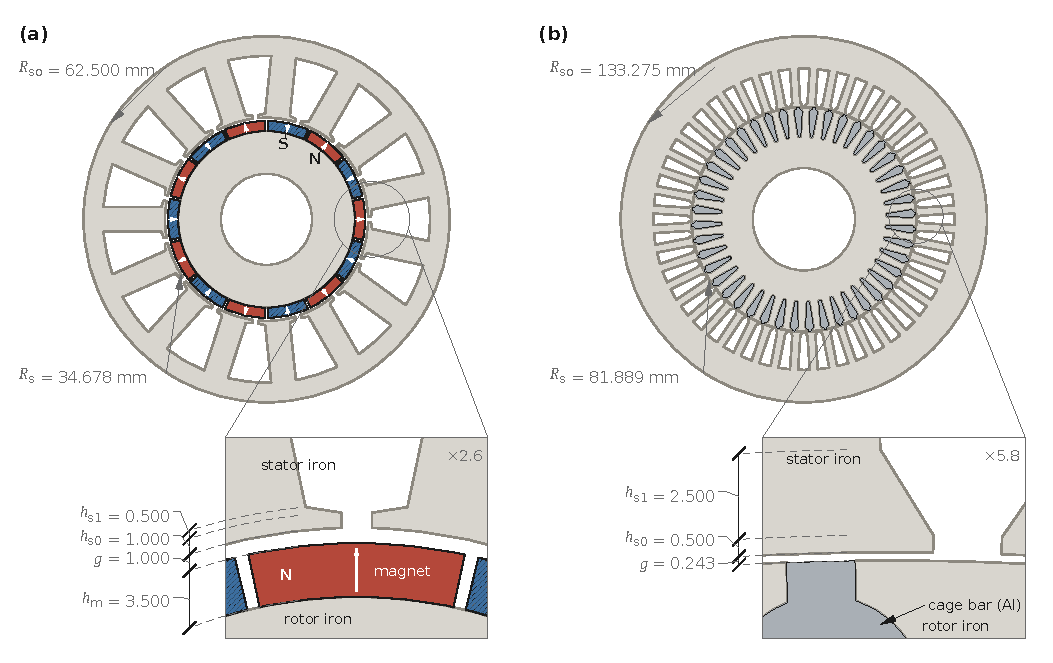
\includegraphics[width=\textwidth,height=0.44\textheight,keepaspectratio]{fig_machines.pdf}
\caption{Cross-sections of the two machines, to scale.
(a) the \SI{750}{\watt} 15-slot/14-pole surface-mounted PMSM validated
in this paper, with its fourteen-sector magnet ring and
\SI{2}{\milli\metre} slot openings; (b) the \SI{18.5}{\kilo\watt}
48-slot/44-bar cage induction machine whose air-gap geometry is given
in Appendix~\ref{app:im}, shown
because the contrast governs Section~\ref{sub:v1}: the annulus condensed
here spans air \emph{and} magnet and is logarithmically thick, that of
(b) is a bare \SI{0.243}{\milli\metre} gap. The insets magnify one slot
and its air gap, which would otherwise not be visible at this scale.}
\label{fig:machines}
\end{figure*}

The central result is the condition rather than the operator.
Section~\ref{sec:trace} proves \emph{in closed form} that under a
piecewise-constant bore basis the self-energy of a column grows as
$\ln N$ without bound, verifies that closed form to $1.4\times10^{-6}$
and its predicted slope to four significant figures at three column
widths, with no adjusted quantity anywhere, and shows that the
continuous piecewise-linear basis restores an absolutely convergent
series with a residual tail in $1/N^{2}$ for the price of one line of
code. \emph{Under the discontinuous basis the condensed operator has no
limit; the truncation selects a value instead of approximating one.}
Neither the result nor the diagnostic that exposes it, the ratio of
successive increments, tending to unity for a logarithmic tail and to a
constant below one for a geometric one, is specific to electrical
machines: both apply to any condensation of a surface operator onto a
discontinuous basis.

The operator itself contributes three things. It spans air and magnet as
a single surface map with the magnetisation entering as a source term,
so the magnet region requires no matching of its own. It is invariant
with rotor position whenever one bounding surface is smooth, as it is on
a surface-mounted-magnet rotor, which is what allows a \num{721}-position
cogging sweep to cost one factorisation and \num{721}
back-substitutions; that property does not survive two slotted
surfaces. And it removes the
fitted air-gap quantities instead of re-identifying them: slot-opening
fringing, the tangential field, the radial attenuation of the slot
harmonics and the inter-polar leakage all emerge from the solution, and
three constants required by the lumped counterpart disappear with them.
The claim is bounded to the air gap, and Section~\ref{sub:fitted} states
exactly which constants it does and does not cover. The coupled system
is solved by an exact Newton scheme whose Jacobian uses the differential
reluctance
$\mathcal{R}_{\mathrm{d}}=(\ell/A)\,\mathrm{d}H/\mathrm{d}B$: nine to
fifteen iterations reach a relative residual of $5\times10^{-13}$, where
the successive substitution standard in the reluctance-network
literature stops at $6.9\times10^{-4}$ after \num{500}.

Two further results concern not the formulation but the ground it is
measured on. A five-test procedure is proposed for auditing the
finite-element reference without re-solving it, and on this machine it
is what establishes the unphysical spatial order and the factor of 87
quoted above. And the formulation is delimited, which we regard as a
result rather than a caveat: the first slot sideband and the cogging
torque are governed by a tooth-tip corner singularity, they are
mesh-dependent in the reference as much as in the network, and they are
reported as bounds. Section~\ref{sec:bounds} shows this to be the
\emph{same} failure of regularity as the harmonic tail of
Section~\ref{sec:trace}, seen in the mesh basis instead of the Fourier
basis, two projections of one phenomenon, not two separate
limitations.

Section~\ref{sec:dtn} develops the operator and establishes its
symmetry, its semi-definiteness and the rank condition that follows;
Section~\ref{sec:trace} treats trace conformity and is the theoretical
core; Section~\ref{sec:mesh} details the coupling to the nonlinear mesh
and the cost of the resulting chain; Section~\ref{sec:methods} sets out
the validation protocol and Section~\ref{sec:pmsm} the validation
itself. Section~\ref{sec:closures} compares the operator with the
classical closures it replaces, Section~\ref{sec:audit} audits the
reference, and Section~\ref{sec:bounds} states the bounds of validity.


%=======================================================================

%======================================================================
\section{The Dirichlet-to-Neumann Air-Gap Operator}
\label{sec:dtn}

% PROVENANCE : MEC_DtN_paper_v2.tex l. 486-847 et 1002-1018, reprise.
% La sous-section "doubly slotted case" (l. 848-1001) est RETIREE :
% elle est la section 2 de l'article compagnon.
% AJOUTS : verification T7 (aimantation radiale) apres eq:Mn ;
% le paragraphe de la queue logarithmique POSE le probleme et le
% renvoie a la section 3, au lieu de le declarer resolu.


\subsection{Two-Layer Operator for the Air Gap and Magnet Annulus}
\label{sub:twolayer}

\subsubsection{Boundary-Value Problem Statement}

Consider the annulus bounded by the rotor back-iron surface $r=\rmi$,
the magnet outer surface $r=\Rro$ and the stator bore $r=\Rs$
(Fig.~\ref{fig:annulus}). The region $\rmi \le r \le \Rro$ is occupied
by surface-mounted magnets of recoil permeability $\murec$ and radial
magnetisation $M_r(\theta)$; the region $\Rro \le r \le \Rs$ is air.
Currents are absent from the annulus, so the field derives from a scalar
potential,
\begin{equation}
\bm{H} = -\nabla \varphi .
\label{eq:H}
\end{equation}
The rotor back-iron is taken infinitely permeable, which imposes
\begin{equation}
\varphi(\rmi,\theta) = 0 ,
\label{eq:bc_rotor}
\end{equation}
while the potential on the stator bore, $\varphi(\Rs,\theta) =
u_{\mathrm{s}}(\theta)$, is an unknown carried by the stator reluctance
network. The operator sought returns the radial flux density at the bore
as a linear functional of $u_{\mathrm{s}}$ plus a source term due to the
magnets.

\emph{This is a linearity assumption, and it is the same one criticised
in Section~\ref{sec:closures} in the subdomain and hybrid families.} It
is made here on the rotor side, on a yoke \SI{14.678}{\milli\metre}
thick, and it should be bounded rather than asserted. What bounds it is
the magnet layer itself: with $\Um=\ln(\Rro/\rmi)=\num{0.1097}$, the
factor $\coth(n\Um)$ through which the rotor boundary reaches the bore
falls to \num{1.25} at $n=10$ and to \num{1.03} at $n=20$, so beyond the
first few orders the magnet decouples the rotor iron from the surface
and \eqref{eq:bc_rotor} ceases to influence $g_n$. What remains exposed
is the fundamental and the lowest orders. \emph{The bound is geometric,
not magnetic}: the peak rotor-yoke flux density is not exported by any
file of the reference project, so the recoil margin of the iron is not
quantified here. Stating this is the honest form of the assumption.

\begin{figure}[!ht]
\centering
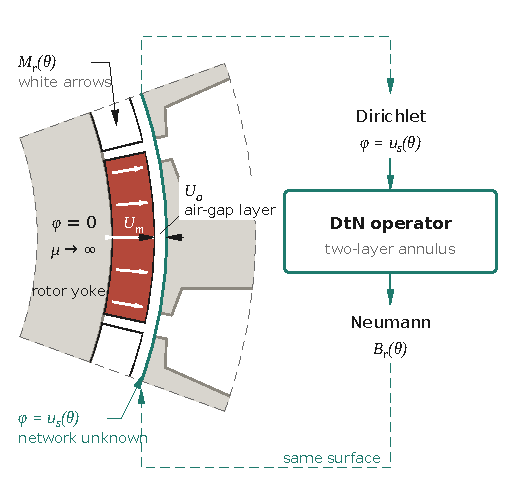
\includegraphics[width=0.98\linewidth]{fig_annulus.pdf}
\caption{Geometry of the two-layer annulus condensed by the operator.
The magnet layer $\rmi\le r\le\Rro$ carries the radial magnetisation
$M_r(\theta)$ and recoil permeability $\murec$; the region
$\Rro\le r\le\Rs$ is air. The rotor back-iron imposes
$\varphi(\rmi,\theta)=0$, while the bore potential
$u_{\mathrm{s}}(\theta)$ is an unknown carried by the stator reluctance
network. The logarithmic thicknesses $\Ua$ and $\Um$ of
\eqref{eq:thick} are the natural coordinates of the two layers. The
block on the right states the map the section constructs: a Dirichlet
datum on the bore returns a Neumann datum. The air gap is drawn
exaggerated.}
\label{fig:annulus}
\end{figure}

\subsubsection{Logarithmic Coordinate and Analytical Layer Solutions}

Laplace's equation in polar coordinates is separable in the logarithmic
radial variable. Writing $v=\ln(r/r_0)$ for a layer of inner radius
$r_0$, the harmonic of order $n$ obeys
$\mathrm{d}^2\varphi_n/\mathrm{d}v^2 - n^2\varphi_n = 0$, so that
$\varphi_n$ is a combination of $\cosh(nv)$ and $\sinh(nv)$. This basis
is preferred to $r^{\pm n}$ for a numerical reason: for the orders
required here ($n$ up to several hundred) the powers $r^{\pm n}$
overflow or underflow in double precision, with $r$ in metres both
occur, $r^{-n}$ overflowing and $r^{+n}$ underflowing, whereas the
hyperbolic form remains well
conditioned provided each layer uses its own local coordinate. Define
the logarithmic thicknesses
\begin{equation}
\Ua = \ln\!\left(\frac{\Rs}{\Rro}\right),
\qquad
\Um = \ln\!\left(\frac{\Rro}{\rmi}\right).
\label{eq:thick}
\end{equation}

\emph{Air-gap layer.} With $v=\ln(r/\Rro)$ and the interface potential
$\varphi_{\mathrm{i},n} = \varphi_n(\Rro)$,
\begin{equation}
\varphi_n^{\mathrm{a}}(v) =
\frac{\varphi_{\mathrm{i},n}\sinh\!\big(n(\Ua-v)\big)
      + u_{\mathrm{s},n}\sinh(nv)}{\sinh(n\Ua)} .
\label{eq:phi_air}
\end{equation}

\emph{Magnet layer.} The constitutive law is
$\bm{B} = \mu_0\murec\bm{H} + \mu_0\bm{M}$, so that
$\nabla\!\cdot\!\bm{B}=0$ gives
$\murec\nabla^2\varphi = \nabla\!\cdot\!\bm{M}$. For a purely radial
magnetisation independent of $r$, $\nabla\!\cdot\!\bm{M}=M_r(\theta)/r$,
and the harmonic of order $n$ admits the particular solution
\begin{equation}
\begin{aligned}
\varphi_{\mathrm{p},n}(r) &= P_n\,r ,\\[1ex]
P_n &=
\begin{cases}
\dfrac{M_n}{\murec\left(1-n^{2}\right)}, & n \neq 1,\\[2ex]
0, & n = 1 .
\end{cases}
\end{aligned}
\label{eq:particular}
\end{equation}
The complete layer solution adds the homogeneous part. Writing
$w=\ln(r/\rmi)$ for the magnet coordinate,
\begin{equation}
\varphi^{\mathrm{m}}_n(w)=C_n\cosh(nw)+A_n\sinh(nw)+P_n\,r ,
\label{eq:magnet_layer}
\end{equation}
so that the rotor-iron condition \eqref{eq:bc_rotor}, imposed at $w=0$,
gives $C_n=-P_n\rmi$ directly, and matching $\varphi_{\mathrm{i},n}$ at
$\Rro$ gives $A_n$ as it appears in \eqref{eq:Br_mag}. \emph{The
lettering matters}: $C_n$ multiplies the hyperbolic cosine and $A_n$ the
hyperbolic sine, and exchanging them changes the radial structure of the
magnet field, hence the leakage factor and the magnet-loss integral of
Section~\ref{sub:pmloss}.

Equation~\eqref{eq:particular} is the only degeneracy of the
formulation, and it deserves an explicit statement rather than a
footnote. The order $n=1$ must be excluded. For every machine with
$p\ge2$ this is harmless: by \eqref{eq:Mn} below, $M_n$ vanishes unless
$n$ is an odd multiple of $p$, so $M_1=0$ and the convention $P_1\equiv0$
removes an indeterminate $0/0$ that would otherwise arise in
floating-point arithmetic. For a two-pole machine, however, $n=1=p$ and
$M_1\neq0$: the particular solution is then of the form $r\ln r$ and the
expressions below do not apply. The two-pole case is outside the scope
of this paper.

\subsubsection{Magnetisation Spectrum of the Magnet Layer}

For alternately magnetised arcs of relative span $\alpha_{\mathrm{m}}$
(magnet arc divided by pole pitch) and remanence $B_{\mathrm{r}}$, the
radial magnetisation contains only odd multiples of $p$. The spectrum
below and the two-layer open-circuit field that follows from it are the
classical results of Zhu and Howe for the open-circuit and
armature-reaction fields of a brushless permanent-magnet
motor~\cite{zhu1993a,zhu1993b}; they are restated here to fix the
notation on which the operator is built, and no novelty is claimed for
them:
\begin{equation}
M_n =
\begin{cases}
\dfrac{4B_{\mathrm{r}}}{\mu_0\,m\,\pi}\,
\sin\!\left(\dfrac{m\pi\alpha_{\mathrm{m}}}{2}\right),
& n = m\,p,\ m\ \text{odd},\\[2ex]
0, & \text{otherwise.}
\end{cases}
\label{eq:Mn}
\end{equation}
All integer orders are nevertheless retained in the operator: slotting
excites orders that are not multiples of $p$, and it is precisely their
transfer through the annulus that a permeance function cannot describe.

Equation~\eqref{eq:Mn} assumes the magnetisation to be purely radial,
which is an assumption about the machine and not about the method, and
it is worth verifying rather than declaring. A sintered rare-earth arc
of relative span \num{0.94} in a fourteen-pole rotor is often magnetised
\emph{parallel}, which would add a $M_\theta$ component absent from
\eqref{eq:Mn}. The reference model used throughout this paper declares
a cylindrical coordinate system with direction components
$(1,0)$: the magnetisation of the reference is radial, and the
hypothesis of \eqref{eq:Mn} is exactly the one the reference makes.

\subsubsection{Interface Continuity Conditions and Response Coefficients}

Continuity of the radial flux density at $r=\Rro$,
\begin{equation}
-\mu_0\,\frac{\partial\varphi^{\mathrm{a}}}{\partial r}\bigg|_{\Rro}
= -\mu_0\murec\,\frac{\partial\varphi^{\mathrm{m}}}{\partial r}\bigg|_{\Rro}
+ \mu_0 M_r ,
\label{eq:continuity}
\end{equation}
eliminates $\varphi_{\mathrm{i},n}$ in favour of the bore potential. The
result is affine,
\begin{equation}
\varphi_{\mathrm{i},n} = \alpha_n\,u_{\mathrm{s},n} + \beta_n ,
\label{eq:phii}
\end{equation}
with, writing $D_n = (n/\Rro)\big[\coth(n\Ua)+\murec\coth(n\Um)\big]$,
\begin{align}
\alpha_n &= \frac{1}{D_n}\,\frac{n/\Rro}{\sinh(n\Ua)}\notag\\
 &= \big[\cosh(n\Ua)+\murec\sinh(n\Ua)\coth(n\Um)\big]^{-1},
\label{eq:alpha}\\[1ex]
\beta_n &= \frac{1}{D_n}\Bigl[\murec\frac{n\,P_n}{\Rro}
 \Bigl(\Rro\coth(n\Um)-\frac{\rmi}{\sinh(n\Um)}\Bigr)\notag\\
 &\qquad\qquad\quad -\murec P_n + M_n\Bigr].
\label{eq:beta}
\end{align}
The two terms have distinct meanings: $\alpha_n$ is the transfer of the
stator-side excitation through the two layers, and $\beta_n$ the
contribution of the magnets seen at the interface. The $\coth$ and
$1/\sinh$ combinations in $D_n$ are the classical Steklov--Poincar\'e~\cite{quarteroni1999}
symbols of an annulus; their appearance here for a \emph{two-layer}
region, with $\murec$ weighting the magnet contribution, is what
generalises the single-layer air-gap operator.

\subsubsection{Bore Admittance and Equivalent Source Term}

Substituting \eqref{eq:phii} into \eqref{eq:phi_air} and evaluating
$B_r = -\mu_0\,\partial\varphi/\partial r$ at $r=\Rs$ yields the
harmonic form of the operator,
\begin{equation}
B_{r,n}(\Rs) = g_n\,u_{\mathrm{s},n} + b_n ,
\label{eq:bore}
\end{equation}
with
\begin{equation}
\begin{aligned}
g_n &= -\mu_0\,\frac{n}{\Rs}\,
       \frac{\cosh(n\Ua)-\alpha_n}{\sinh(n\Ua)} ,\\[1ex]
b_n &= \ \ \mu_0\,\frac{n}{\Rs}\,\frac{\beta_n}{\sinh(n\Ua)} .
\end{aligned}
\label{eq:gnbn}
\end{equation}
Equation~\eqref{eq:bore} \emph{is} the Dirichlet-to-Neumann map: a
Dirichlet datum $u_{\mathrm{s}}$ on the bore produces a Neumann datum
$B_r$, with an inhomogeneous part $b_n$ carrying the magnets.

\subsubsection{Projection onto the Network Surface Nodes}
\label{sub:proj}

The stator network carries $M_{\mathrm{s}}$ surface nodes, node $k$
spanning the arc $[\theta_k-\Delta\theta_k/2,\
\theta_k+\Delta\theta_k/2]$ at $r=\Rs$ and holding a uniform potential
$U_k$. Projecting a piecewise-constant potential onto the Fourier basis
gives the rectangular operators
\begin{equation}
\begin{aligned}
W^{\mathrm{c}}_{nk} &= \frac{2}{n\pi}
\sin\!\left(\frac{n\Delta\theta_k}{2}\right)\cos(n\theta_k),\\
W^{\mathrm{s}}_{nk} &= \frac{2}{n\pi}
\sin\!\left(\frac{n\Delta\theta_k}{2}\right)\sin(n\theta_k) .
\end{aligned}
\label{eq:W}
\end{equation}
Throughout, a bore quantity $f(\theta)$ is expanded as
$f(\theta)=\sum_{n\ge1}\big(f_n^{\mathrm{c}}\cos n\theta
+ f_n^{\mathrm{s}}\sin n\theta\big)$, with real coefficients; this
convention fixes the factors in \eqref{eq:Ymat} and in the torque sum
\eqref{eq:torque}. The flux entering the iron through the surface nodes
then reads
\begin{equation}
\bm{\Phi}_{\mathrm{s}} = \bm{Y}\,\bm{U}_{\mathrm{s}}
+ \bm{i}_{\mathrm{src}}(\phi) ,
\label{eq:Y}
\end{equation}
where, with $L$ the active length,
\begin{align}
\bm{Y} &= \pi L \Rs
\Bigl[(\bm{W}^{\mathrm{c}})^{\!\top}\!\operatorname{diag}(\bm{g})\,
\bm{W}^{\mathrm{c}}\notag\\
&\qquad\quad
+(\bm{W}^{\mathrm{s}})^{\!\top}\!\operatorname{diag}(\bm{g})\,
\bm{W}^{\mathrm{s}}\Bigr],
\label{eq:Ymat}\\[1.5ex]
\bm{i}_{\mathrm{src}}(\phi) &= \pi L \Rs
\Bigl[(\bm{W}^{\mathrm{c}})^{\!\top}\!
\big(\bm{b}\odot\cos(\bm{n}\phi)\big)
+(\bm{W}^{\mathrm{s}})^{\!\top}\!
\big(\bm{b}\odot\sin(\bm{n}\phi)\big)\Bigr],
\label{eq:isrc}
\end{align}
$\phi$ being the rotor position and $\odot$ the elementwise product.

\subsection{Mathematical Properties of the Operator}
\label{sub:props}

\paragraph{Symmetry.}
$\bm{Y}$ is symmetric by construction \eqref{eq:Ymat}, being a
congruence of a diagonal matrix. Reciprocity of the magnetostatic
problem is therefore satisfied exactly at the discrete level, not merely
in the limit.

\paragraph{Definiteness and null space.}
From the closed form in \eqref{eq:alpha}, and since $\Ua>0$, $\Um>0$ and
$\murec>0$ imply $\sinh(n\Ua)>0$ and $\coth(n\Um)>0$, one has
$0<\alpha_n<\big[\cosh(n\Ua)\big]^{-1}$ for every $n\ge1$. Hence
$\cosh(n\Ua)-\alpha_n>0$ and therefore $g_n<0$ for every $n\ge1$. The
congruence \eqref{eq:Ymat} makes $\bm{Y}$ negative
\emph{semi}-definite. It is not definite, and the deficiency is exactly
one dimension. On a uniform bore grid of $M_{\mathrm{s}}$ segments the
angular sum in \eqref{eq:W} vanishes for every $n$ that is not a
multiple of $M_{\mathrm{s}}$, while $\sin(n\Delta\theta/2)$ vanishes for
every $n$ that is; hence $\bm{W}^{\mathrm{c}}\bm{1} =
\bm{W}^{\mathrm{s}}\bm{1} = \bm{0}$ and
\begin{equation}
\bm{Y}\,\bm{1} = \bm{0} .
\label{eq:nullspace}
\end{equation}
This is the correct physics rather than a defect: raising the whole bore
uniformly against a rotor held at $\varphi=0$ drives no net flux, by
Gauss's law. The operator fixes flux \emph{differences}, not the
potential level, and the gauge must be supplied by the iron network
through its reference node.

Two consequences are practical. First, since
$\operatorname{rank}\bm{Y} = \min(2N,\,M_{\mathrm{s}}-1)$ with $N$ the
number of retained harmonics, the truncation must satisfy
\begin{equation}
N \ \ge\ M_{\mathrm{s}}/2
\label{eq:truncation}
\end{equation}
for the null space to reduce to the constants; below that threshold the
surface block is structurally rank-deficient by $M_{\mathrm{s}}-2N$ and
the coupled system is under-determined on the bore.
Table~\ref{tab:rank} verifies \eqref{eq:truncation} on the test machine.
Condition \eqref{eq:truncation} fixes the rank, but it does not make the
operator convergent, and the distinction matters. For large $n$,
$\alpha_n\to0$ and $g_n\to-\mu_0 n/\Rs$, while
$(W^{\mathrm{c}}_{nk})^2+(W^{\mathrm{s}}_{nk})^2
=\tfrac{4}{n^2\pi^2}\sin^2(n\Delta\theta_k/2)$, so the diagonal entries
of \eqref{eq:Ymat} behave as
\begin{equation}
\begin{aligned}
Y_{kk} &\sim\ -\frac{4\mu_0 L}{\pi}
\sum_n \frac{\sin^2(n\Delta\theta_k/2)}{n}\\[0.5ex]
&=\ -\frac{2\mu_0 L}{\pi}\ln N + O(1).
\end{aligned}
\label{eq:logtail}
\end{equation}
The sum diverges logarithmically. This is not a defect of the algebra
but a property of the trial space: a piecewise-constant bore potential
is discontinuous, its Fourier coefficients decay only as $1/n$, and the
tangential field it implies is singular at every segment boundary. Such
a datum does not belong to $H^{1/2}$, the trace space on which the
Dirichlet-to-Neumann map is bounded.

\begin{table}[!ht]
\centering
\footnotesize
\begin{tabular}{ccc}
\toprule
Harmonics $N$ & $\operatorname{rank}\bm{Y}$ & Null-space dimension \\
\midrule
60  & 120 & 240 \\
120 & 240 & 120 \\
179 & 358 & 2   \\
\textbf{180} & \textbf{359} & \textbf{1} \\
360 & 359 & 1   \\
\bottomrule
\end{tabular}
\caption{Rank of the bore operator, $M_{\mathrm{s}}=360$, PMSM data. The
null space reduces to the constants only for $N\ge M_{\mathrm{s}}/2$.}
\label{tab:rank}
\end{table}

The consequence deserves to be stated plainly, because the literature
does not state it. Condition~\eqref{eq:truncation} fixes the \emph{rank}
of the operator; it says nothing about its \emph{limit}. Under the
truncation $N=\lfloor M_{\mathrm{s}}/2\rfloor$ that the implementation
enforces, the diagonal of $\bm{Y}$ is finite because the sum has been
stopped, not because it converges, and a matrix entry whose value
depends on where the sum was stopped is not a property of the geometry.
Section~\ref{sec:trace} takes this up: it establishes
\eqref{eq:logtail} in closed form, including the additive constant,
verifies it numerically over four decades, and shows what has to change
in the trial space for the operator to have a limit. Until that section,
every statement below holds \emph{at fixed truncation}.

Second, once the gauge is fixed and \eqref{eq:truncation} holds, the
coupled matrix $\bm{A}_{\mathrm{ss}}-\bm{Y}$ is symmetric positive
definite for any mesh and no stabilisation is required, but this is a
property of the \emph{coupled} system, not of $\bm{Y}$ alone.


\paragraph{Rotor-position invariance.}
The rotor position $\phi$ appears only in $\bm{i}_{\mathrm{src}}$
through \eqref{eq:isrc}. The dense matrix $\bm{Y}$, and therefore its
factorisation or its Schur complement onto the interior nodes, is
computed once for a machine and reused at every position. A sweep of
$N_\phi$ positions costs one factorisation and $N_\phi$
back-substitutions.

\paragraph{Field in the annulus.}
Once $\bm{U}_{\mathrm{s}}$ is known, the field at any radius follows in
closed form. In the air gap, at $v=\ln(r/\Rro)$, and with the sign
convention of \eqref{eq:W},
\begin{align}
B_r(r,\theta) &= -\mu_0\sum_{n\ge1}\frac{n}{r}\,
\frac{\cosh(nv)-\alpha_n\cosh\!\big(n(\Ua-v)\big)}{\sinh(n\Ua)}\notag\\
&\quad\times\big(u^{\mathrm{c}}_{\mathrm{s},n}\cos n\theta
    + u^{\mathrm{s}}_{\mathrm{s},n}\sin n\theta\big)
+ B_r^{\mathrm{mag}},
\label{eq:Br_gap}\\[1ex]
B_t(r,\theta) &= \ \ \mu_0\sum_{n\ge1}\frac{n}{r}\,
\frac{\sinh(nv)+\alpha_n\sinh\!\big(n(\Ua-v)\big)}{\sinh(n\Ua)}\notag\\
&\quad\times\big(u^{\mathrm{s}}_{\mathrm{s},n}\cos n\theta
     - u^{\mathrm{c}}_{\mathrm{s},n}\sin n\theta\big)
+ B_t^{\mathrm{mag}}.
\label{eq:Bt_gap}
\end{align}
The magnet contributions $B^{\mathrm{mag}}_{r,t}$ have the same form
with $\alpha_n u_{\mathrm{s},n}$ replaced by $\beta_n$ and are omitted
for brevity. The tangential component \eqref{eq:Bt_gap}, which a network
of radial branches cannot produce at all, is obtained here at no
additional cost; it is what makes a Maxwell-stress torque available
directly from the surface potentials.

Inside the magnet, with $w=\ln(r/\rmi)$, the complete radial component
of the order-$n$ harmonic is
\begin{equation}
\begin{aligned}
B_{r,n}^{\mathrm{m}}(r) = &-\mu_0\murec\,\frac{n}{r}
\Big[A_n\cosh(nw)+C_n\sinh(nw)\Big]\\ &- \mu_0\murec P_n + \mu_0 M_n ,
\end{aligned}
\label{eq:Br_mag}
\end{equation}
with $C_n=-P_n\rmi$ from \eqref{eq:bc_rotor} and
$A_n=\big[\varphi_{\mathrm{i},n}-P_n\Rro-C_n\cosh(n\Um)\big]/\sinh(n\Um)$
from the match at $\Rro$. The stator-driven part is the $A_n$ term;
retaining $C_n$ and $P_n$ matters for the magnet-loss integral of
Section~\ref{sub:pmloss}, where they carry the radial variation of the
field through the magnet thickness. Both the leakage factor and the
magnet eddy-current losses follow from \eqref{eq:Br_mag} without further
hypothesis.


\subsection{Electromagnetic Torque}

With $B_r$ and $B_t$ available as Fourier series at any radius, the
Maxwell stress integral collapses to a Parseval sum. With the real
expansion fixed in Section~\ref{sub:proj},
\begin{equation}
T = \frac{\pi L r^2}{\mu_0}
\sum_{n\ge1}\left(B_{r,n}^{\mathrm{c}}B_{t,n}^{\mathrm{c}}
+ B_{r,n}^{\mathrm{s}}B_{t,n}^{\mathrm{s}}\right),
\label{eq:torque}
\end{equation}
evaluated on a circle inside the air gap. No surface integration and no
mesh-dependent contour are involved, which is what makes the torque
insensitive to the choice of integration path, a known weakness of
Maxwell-stress evaluation on a finite-element mesh.

%=======================================================================

%======================================================================

\section{Trace Conformity of the Condensed Operator}
\label{sec:trace}

Section~\ref{sec:dtn} derived the operator of the annulus exactly. What
enters a reluctance network, however, is never that operator: it is its
restriction to a finite-dimensional space of bore potentials, condensed
into a symmetric matrix. The choice of that space is usually treated as
a discretisation detail, to be refined until the answer stops moving.
It is not. We show here that the piecewise-constant choice, the one
every reluctance network makes, because a network node carries one
potential, places the bore potential outside the space on which the
operator is bounded, and that the resulting matrix has no limit. The
remedy costs one line of code; the diagnostic that detects the problem
costs four runs and no theory.

\subsection{Piecewise-Constant Projection and Its Spectral Tail}
\label{sub:p0tail}

Let the bore be divided into $M_{\mathrm{s}}$ columns, column $i$
spanning an arc of angular width $d$ centred on $\theta_i$, and let the
bore potential be expanded on a basis $\{\psi_i\}$. With $g_n$ the bore
admittance of order $n$ from~\eqref{eq:gnbn} and $W_n(i)$ the order-$n$
Fourier coefficient of $\psi_i$, the condensed matrix
of~\eqref{eq:Ymat} truncated at order $N$ is a sum of $N$ rank-one
terms, and its diagonal is the energy
\begin{equation}
Y(i,i)\;=\;\sum_{n\le N} g_n\,\bigl|W_n(i)\bigr|^{2}.
\label{eq:energy}
\end{equation}
Throughout this section the energy is reported as $-Y(i,i)>0$: the sign
is fixed by $g_n<0$, established in Section~\ref{sub:props}, and is
dropped so that the tables of this section carry positive entries.

Two facts about the two factors decide everything. First, the bore
admittance grows linearly: once $n\gg 1/\Ua$ the kernel degenerates,
$\coth(n\Ua)\to1$, and $\hat{g}_n\to-\mu_0 L\pi n$. \emph{The circumflex
matters.} Equation~\eqref{eq:gnbn} defines $g_n$ as a flux density per
unit potential, in \si{\henry\per\metre\squared}; what enters
\eqref{eq:energy}, and what grows linearly, is the \emph{assembled}
admittance of order $n$,
$\hat{g}_n=\pi L\Rs\,g_n$, in \si{\henry}. The two differ by the factor
$\pi L\Rs$ of \eqref{eq:Ymat} and by sign, and a reader checking
\eqref{eq:energy} against \eqref{eq:gnbn} without this distinction
obtains the wrong power of $\Rs$. Second, the indicator
function of an arc has Fourier coefficients that decay only as $1/n$,
\begin{equation}
W_n(i)\;=\;\frac{2}{n\pi}\,\sin\!\Bigl(\frac{nd}{2}\Bigr)\,
\mathrm{e}^{-\mathrm{i}n\theta_i},
\label{eq:Wn_p0}
\end{equation}
so that $g_n|W_n|^{2}$ decays as $1/n$ and not faster. Substituting
in~\eqref{eq:energy},
\begin{equation}
-Y(i,i)\;=\;\frac{4\mu_0 L}{\pi}\sum_{n\le N}\frac{1}{n}\,
\sin^{2}\!\Bigl(\frac{nd}{2}\Bigr).
\label{eq:p0self}
\end{equation}
Since $\sin^{2}$ averages to one half, the summand behaves as $1/(2n)$:
the series is harmonic and diverges.

Two features of this divergence explain why it has gone unnoticed. It is
confined to the diagonal, the off-diagonal entries carry an extra
$\cos(n\Delta\theta)$ and converge, as Section~\ref{sub:p0closed} shows
in closed form, so the condensed matrix never blows up as a whole and
every finite truncation returns a perfectly ordinary, finite, symmetric
matrix. And it is logarithmic, so each doubling of $N$ adds the same
fixed amount: the drift never stops, but it never accelerates either.
A quantity that moves by a constant amount per doubling and never
settles is exactly what a slowly converging quantity looks like from a
distance. It is not one.

\subsection{Closed-Form Expression of the Logarithmic Divergence}
\label{sub:p0closed}

The behaviour just described can be stated exactly rather than
asymptotically. \emph{One preliminary is needed, and it fixes the scope
of what follows.}

The proposition below is proved on the \emph{asymptotic} kernel
$\hat{g}_n^{\,\mathrm{asym}}=-\mu_0L\pi n$, not on the exact bore
admittance of \eqref{eq:gnbn}. Write the exact kernel as
\begin{equation}
\hat{g}_n=\hat{g}_n^{\,\mathrm{asym}}+\Delta_n,
\qquad
\Delta_n=-\mu_0L\pi n\left[\frac{\cosh(n\Ua)-\alpha_n}{\sinh(n\Ua)}-1\right].
\label{eq:kernelsplit}
\end{equation}
Since $\coth(x)-1=2e^{-2x}/(1-e^{-2x})$ and
$0<\alpha_n<1/\cosh(n\Ua)$, the bracket is $O(e^{-2n\Ua})$ and hence
$\Delta_n=O\!\left(n\,e^{-2n\Ua}\right)$. With $|W_n|=O(1/n)$ in the
piecewise-constant basis, the correction series
$\sum_n \Delta_n|W_n|^2$ therefore converges \emph{absolutely}, its terms
decaying exponentially.

Two consequences follow, and they are not the same. \emph{The divergence
is a property of the exact operator}: it comes from
$\hat{g}_n^{\,\mathrm{asym}}$, which the correction cannot cancel because
the correction converges. \emph{The additive constant is exact for the
asymptotic kernel and asymptotically exact for the true one}, the
difference being a convergent constant that depends on the annulus
through $\Ua$. Table~\ref{tab:p0tail} verifies the closed form against
its own numerical summation on the asymptotic kernel; what it does
\emph{not} do is verify that the condensed operator of a real annulus
carries that same constant, and the distinction is stated here rather
than left for a reader to find.

\begin{proposition}
\label{prop:closed}
Let columns $i$ and $j$ have angular widths $d_i$, $d_j$ and angular
separation $\Delta\theta$, and write
$a_{1,2}=\tfrac12(d_i-d_j)\pm\Delta\theta$,
$a_{3,4}=\tfrac12(d_i+d_j)\pm\Delta\theta$. In the degenerate regime
$n\gg1/\Xg$, the truncated entry of the condensed operator satisfies, as
$N\to\infty$:
\begin{enumerate}[label=(\alph*),leftmargin=*]
\item off the diagonal, the series converges, with limit
\begin{equation}
\begin{aligned}
Y(i,j)=\frac{\mu_0 L}{\pi}\Bigl[
&-\ln\bigl|2\sin\tfrac{a_1}{2}\bigr|
 -\ln\bigl|2\sin\tfrac{a_2}{2}\bigr|\\
&+\ln\bigl|2\sin\tfrac{a_3}{2}\bigr|
 +\ln\bigl|2\sin\tfrac{a_4}{2}\bigr|\Bigr];
\end{aligned}
\label{eq:closed_off}
\end{equation}
\item on the diagonal $(d_i=d_j=d,\ \Delta\theta=0)$, the series
diverges, with
\begin{equation}
-Y(i,i)=\frac{2\mu_0 L}{\pi}
\Bigl[\ln N+\gamma+\ln\bigl|2\sin\tfrac{d}{2}\bigr|\Bigr]+o(1),
\label{eq:closed_diag}
\end{equation}
$\gamma$ being the Euler--Mascheroni constant. No truncation bounds it.
\end{enumerate}
\emph{Scope.} Statements (a) and (b) hold exactly for the asymptotic
kernel $\hat{g}_n^{\,\mathrm{asym}}$. For the exact kernel of
\eqref{eq:gnbn}, the divergence of (b) and the convergence of (a) are
unchanged, by \eqref{eq:kernelsplit}; the additive constants acquire a
correction that is finite and independent of $N$.
\end{proposition}

\begin{proof}
Write the general entry as
$\frac{4\mu_0L}{\pi}\sum_{n\le N}\frac1n
\sin\frac{nd_i}{2}\sin\frac{nd_j}{2}\cos(n\Delta\theta)$ and expand the
product of three circular functions,
$\sin A\sin B\cos C=\tfrac14[\cos(A-B+C)+\cos(A-B-C)
-\cos(A+B+C)-\cos(A+B-C)]$. Each of the four resulting series has the
form $\sum_{n\le N}\cos(n\alpha)/n$, whose partial sums satisfy
$\sum_{n\le N}\cos(n\alpha)/n=-\ln|2\sin(\alpha/2)|+o(1)$ for
$\alpha\not\equiv0 \pmod{2\pi}$, and
$\sum_{n\le N}1/n=\ln N+\gamma+o(1)$ for $\alpha\equiv0$. Off the
diagonal all four arguments are non-zero, giving~\eqref{eq:closed_off}.
On the diagonal $a_1=a_2=0$, so two of the four series are the harmonic
series and the remaining two contribute
$\ln|2\sin(d/2)|$, giving~\eqref{eq:closed_diag}.
\end{proof}

Table~\ref{tab:p0tail} verifies both statements numerically. The
off-diagonal series matches~\eqref{eq:closed_off} to
$2.3\times10^{-5}$ at $N=10^{7}$. On the diagonal, the summed value
matches~\eqref{eq:closed_diag} to $1.4\times10^{-6}$, and, the
independent check that matters, the increment per decade converges to
$(2\mu_0L/\pi)\ln 10=\num{3.0354e-7}$, which is the predicted slope and
contains no adjustable quantity. Repeating the test at three column
widths shows that the additive constant tracks $\ln|2\sin(d/2)|$: the
closed form is not a two-parameter fit that happens to work.

\begin{table}[!ht]
\centering
\begin{threeparttable}
\footnotesize
\begin{tabular}{rrrr}
\multicolumn{4}{l}{\emph{(a) Off diagonal, $d_i=d_j=\SI{6}{\milli\radian}$, $\Delta\theta=\SI{50}{\milli\radian}$}}\\
\toprule
$N$ & summed & \eqref{eq:closed_off} & rel.\ dev. \\
\midrule
$10^{3}$ & \num{-1.0569e-9} & \num{-9.5624e-10} & \num{1.05e-1}\\
$10^{4}$ & \num{-1.2005e-9} & \num{-9.5624e-10} & \num{2.55e-1}\\
$10^{5}$ & \num{-1.0085e-9} & \num{-9.5624e-10} & \num{5.46e-2}\\
$10^{6}$ & \num{-9.5646e-10} & \num{-9.5624e-10} & \num{2.26e-4}\\
$10^{7}$ & \num{-9.5622e-10} & \num{-9.5624e-10} & \num{2.30e-5}\\
\bottomrule
\end{tabular}

\vspace{3mm}

\begin{tabular}{rrrrr}
\multicolumn{5}{l}{\emph{(b) Diagonal, $d=\SI{6}{\milli\radian}$; increment per decade at $N=10^{7}$}}\\
\toprule
$N$ & summed & \eqref{eq:closed_diag} & rel.\ dev. & incr./decade \\
\midrule
$10^{3}$ & \num{3.2127e-7} & \num{3.1229e-7} & \num{2.87e-2} & ---\\
$10^{4}$ & \num{6.1648e-7} & \num{6.1583e-7} & \num{1.05e-3} & \num{2.9521e-7}\\
$10^{5}$ & \num{9.1936e-7} & \num{9.1937e-7} & \num{9.52e-6} & \num{3.0288e-7}\\
$10^{6}$ & \num{1.2229e-6} & \num{1.2229e-6} & \num{7.69e-6} & \num{3.0356e-7}\\
$10^{7}$ & \num{1.5265e-6} & \num{1.5265e-6} & \num{1.37e-6} & \num{3.0353e-7}\\
\midrule
\multicolumn{5}{l}{$d=\SI{12}{\milli\radian}$: rel.\ dev.\ \num{3.83e-7}, incr.\ \num{3.0353e-7}}\\
\multicolumn{5}{l}{$d=\SI{24}{\milli\radian}$: rel.\ dev.\ \num{2.94e-7}, incr.\ \num{3.0353e-7}}\\
\bottomrule
\end{tabular}

\vspace{3mm}

\begin{tabular}{rrrr}
\multicolumn{4}{l}{\emph{(c) Diagonal on the \textbf{exact} kernel,
$d=\SI{6}{\milli\radian}$}}\\
\toprule
$N$ & asymptotic & exact & incr./decade, exact \\
\midrule
$10^{4}$ & \num{6.1648e-7} & \num{7.9039e-7} & \num{2.9525e-7}\\
$10^{5}$ & \num{9.1936e-7} & \num{1.0933e-6} & \num{3.0288e-7}\\
$10^{6}$ & \num{1.2229e-6} & \num{1.3968e-6} & \num{3.0356e-7}\\
$10^{7}$ & \num{1.5265e-6} & \num{1.7004e-6} & \num{3.0353e-7}\\
\midrule
\multicolumn{4}{l}{correction $\sum\Delta_n|W_n|^2$: \num{1.7391e-7}\,H at
$N=10^{7}$, \num{1.7388e-7} at $10^{3}$}\\
\bottomrule
\end{tabular}
\end{threeparttable}
\caption{Verification of Proposition~\ref{prop:closed} on a
representative thin annulus, taken with the dimensions of the
\SI{18.5}{\kilo\watt} induction machine because the thin-annulus regime
is where the divergence is observable,
$\Xg=\num{2.9719e-3}$, $L=\SI{164.8}{\milli\metre}$. Panels (a) and (b)
use the asymptotic kernel, panel (c) the exact one of
\eqref{eq:gnbn}: the increment per decade is the same to
\SI{0.0000}{\percent}, so the divergence belongs to the operator and not
to the degeneracy, while the correction of \eqref{eq:kernelsplit} is
already acquired at $N=10^{3}$ and shifts the constant by
\SI{1.74e-7}{\henry} without depending on $N$.
Panel~(a): off-diagonal entries converge. Panel~(b): the diagonal does
not, and its increment per decade matches the predicted slope
$(2\mu_0L/\pi)\ln10=\num{3.0354e-7}$ at three column widths.}
\label{tab:p0tail}
\end{table}

\begin{remark}
The normalisation matters when reading such a table. Dividing
$Y(i,i)$ by $\tfrac12\ln N$ does \emph{not} isolate the slope, because
the additive constant $\gamma+\ln|2\sin(d/2)|$ equals $-4.539$ for
$d=\SI{6}{\milli\radian}$ and decays only as $1/\ln N$; at $N=10^{6}$ it
still displaces the ratio by a third. The slope is best read from the
increment per decade, as in Table~\ref{tab:p0tail}.
\end{remark}

The functional-analytic reading of Proposition~\ref{prop:closed} is the
statement we wish to carry forward. The Dirichlet-to-Neumann operator of
the annulus is bounded from $H^{1/2}(\Gamma)$ into $H^{-1/2}(\Gamma)$;
equivalently its energy form is bounded on $H^{1/2}(\Gamma)$, where it
equals $\sum_n g_n|u_n|^{2}$ with $g_n=O(n)$. Finiteness therefore
requires $\sum_n n\,|u_n|^{2}<\infty$, which is precisely the
$H^{1/2}$ seminorm. A piecewise-constant function on the circle has
jumps, so its coefficients decay as $1/n$ and that sum diverges: it lies
in $H^{s}$ only for $s<1/2$. None of this is new as analysis---the
mapping properties of the Steklov--Poincar\'e operator between
$H^{1/2}(\Gamma)$ and $H^{-1/2}(\Gamma)$, and the requirement that a
Galerkin trial space be a subspace of the energy space, are standard in
the boundary-element and domain-decomposition
literature~\cite{mclean2000,steinbach2008,sauter2011}. What is new is
that, within the reluctance-network and air-gap-element literature
surveyed in Section~\ref{sub:positioning}, and to the best of the
authors' knowledge, the trial space a reluctance network imposes has not
been checked against that requirement, and that the check fails. \emph{The piecewise-constant bore potential
is not an element of the trace space of the problem}, and
Proposition~\ref{prop:closed} is the quantitative form of that fact.

This is a defect of \emph{conformity}, not of resolution. Refining the
bore does not repair it, because every refinement produces another
function outside the space. The distinction is not academic: it decides
whether a drifting output should be extrapolated or discarded.


\subsection{Piecewise-Linear Basis and Restoration of Absolute Convergence}
\label{sub:p1}

The repair follows directly from the diagnosis: choose a basis that lies
in $H^{1/2}$. The continuous, piecewise-linear hat function does, and it
remains a legitimate network unknown, since it is still one degree of
freedom per surface node, only its support now spans two columns
instead of one. Its Fourier coefficients are
\begin{equation}
W_n\;=\;\frac{4}{\pi\,n^{2}d}\,\sin^{2}\!\Bigl(\frac{nd}{2}\Bigr),
\label{eq:Wn_p1}
\end{equation}
so $|W_n|^{2}=O(n^{-4})$ and the energy terms $g_n|W_n|^{2}=O(n^{-3})$.
The series is absolutely convergent, with residual tail bounded by
$\sum_{n>N}n^{-3}\sim1/(2N^{2})$. Table~\ref{tab:p1tail} confirms it:
the product of the tail by $N^{2}$ settles at \num{0.0055} over four
decades. \emph{Truncation becomes a choice of precision instead of a
source of bias.}

\begin{table}[!ht]
\centering
\begin{threeparttable}
\footnotesize
\begin{tabular}{rrr}
\toprule
$N$ & residual tail & tail $\times N^{2}$ \\
\midrule
$10^{2}$ & \num{1.7111e-7} & \num{0.001711}\\
$10^{3}$ & \num{4.3355e-9} & \num{0.004335}\\
$10^{4}$ & \num{5.4115e-11} & \num{0.005412}\\
$10^{5}$ & \num{5.4939e-13} & \num{0.005494}\\
$10^{6}$ & \num{5.4918e-15} & \num{0.005492}\\
\bottomrule
\end{tabular}
\end{threeparttable}
\caption{Hat basis: residual tail of the energy series beyond
truncation $N$, same annulus as Table~\ref{tab:p0tail}. The product by
$N^{2}$ settles, confirming the $\sum_{n>N}n^{-3}$ bound.}
\label{tab:p1tail}
\end{table}

The consequence at model level is visible on the case in which the
defect is largest, the doubly slotted annulus of Appendix~\ref{app:im},
and one column of that sweep is worth isolating here because it is
evidence about the \emph{basis} rather than about the machine. Removing
the slotting from that annulus leaves a smooth bore, on which the
surface potential carries no jump. In the hat basis the condensed
reactance of that smooth bore is then \emph{rigorously constant}:
\SI{81.270}{\ohm} at $N_h=512$ and \SI{81.270}{\ohm} at
$N_h=\num{8192}$, unchanged to five figures over a factor of sixteen in
truncation. In the piecewise-constant basis the same smooth bore drifts
by \SI{0.15}{\percent} over the same sweep.

That contrast is the most direct evidence available for
Proposition~\ref{prop:closed}, and it isolates the mechanism from every
other source of error. The geometry is identical, the operator is
identical, the tiling is identical; only the basis differs, and only one
of the two represents a jump-free potential exactly. The residual drift
of the piecewise-constant basis on a surface with nothing to resolve is
projection error and nothing else. What the same sweep does to the
\emph{slotted} bore, and what the ratio of the two then is, are
properties of that machine rather than of the basis and are outside the
scope of this paper.

\subsection{Numerical Diagnostic Based on the Ratio of Successive Increments}
\label{sub:ratios}

Proposition~\ref{prop:closed} also yields a test that requires neither
the closed form nor any knowledge of the operator. Let $Q(N)$ be any
output of the condensed model and
$\Delta_k=Q(2^{k}N_0)-Q(2^{k-1}N_0)$ the increment between successive
doublings of the truncation. If $Q$ inherits a logarithmic tail, each
doubling contributes the same amount and
$\Delta_{k+1}/\Delta_k\to1$. If $Q$ converges geometrically with ratio
$\rho<1$, then $\Delta_{k+1}/\Delta_k\to\rho$. The two regimes are
distinguished by four runs.

Applied to the magnetising reactance of the slotted annulus, the
piecewise-constant basis gives \num{0.791}, \num{0.874}, \num{0.902}
, tending to unity, the logarithmic signature, and the hat basis gives
\num{0.138}, \num{0.298}, \num{0.304}, a geometric ratio near
\num{0.3} (Table~\ref{tab:trunc}). The test is not
specific to air gaps: it applies to any condensation of a surface
operator onto a discontinuous basis, and we recommend reporting it
alongside any truncation sweep.

\begin{table*}[!t]
\centering
\begin{threeparttable}
\footnotesize
\begin{tabular}{rrrrr}
\toprule
$N_h$ & $\Delta$ p.c.\ (\si{\ohm}) & ratio
      & $\Delta$ hat (\si{\ohm}) & ratio \\
\midrule
\num{1024} & \num{1.1935} & \num{0.791} & \num{0.3155} & \num{0.138}\\
\num{2048} & \num{0.9444} & \num{0.874} & \num{0.0436} & \num{0.298}\\
\num{4096} & \num{0.8252} & \num{0.902} & \num{0.0130} & \num{0.304}\\
\num{8192} & \num{0.7443} & , & \num{0.0040} &, \\
\midrule
\multicolumn{5}{l}{\emph{Truncation unlocked from the tiling}, PMSM,
$M_{\mathrm{s}}=\num{1080}$ fixed\tnote{b}}\\
$N_h$ & \multicolumn{2}{c}{$\ln N+\gamma+\ln|2\sin(d/2)|$}
      & \multicolumn{2}{c}{$B_{g1}$ (\si{\tesla}), dev.}\\
\num{540}  & \multicolumn{2}{c}{\num{1.7219}} & \multicolumn{2}{c}{\num{1.07865}\quad ---}\\
\num{1080} & \multicolumn{2}{c}{\num{2.4151}} & \multicolumn{2}{c}{\num{1.07978}\quad $+0.11\%$}\\
\num{2160} & \multicolumn{2}{c}{\num{3.1082}} & \multicolumn{2}{c}{\num{1.08085}\quad $+0.20\%$}\\
\num{4320} & \multicolumn{2}{c}{\num{3.8014}} & \multicolumn{2}{c}{\num{1.08175}\quad $+0.29\%$}\\
\bottomrule
\end{tabular}
\begin{tablenotes}[flushleft]\footnotesize
\item The swept
quantity is the condensed magnetising reactance of the doubly slotted
annulus of Appendix~\ref{app:im}, at fixed tiling $n_T=17$, $n_O=4$ and
$\Xg=\num{2.9719e-3}$. Only the increments are reported here; the
reactance itself, its converged value and the slotting ratio derived
from it are outside the scope of this paper.
\item[b] The lower panel tests the prediction of
Section~\ref{sub:v1} on the permanent-magnet machine itself. Holding the
tiling at $M_{\mathrm{s}}=\num{1080}$ and releasing $N_h$ from the
$N=M_{\mathrm{s}}/2$ constraint, the bracket resumes its growth, by
\SI{120.8}{\percent} over the sweep, reproducing
$\ln 10=\num{2.302585}$ to \SI{-0.0000}{\percent}, and $B_{g1}$ drifts
monotonically instead of settling. At $N_h=M_{\mathrm{s}}/2$ the released
chain reproduces the locked one to the last bit
(\SI{0}{\tesla} difference), so the port changed the truncation and
nothing else. The sweep stops at $N_h=4M_{\mathrm{s}}$: the projection
$W(n)\propto\sin(nd/2)$ vanishes at multiples of $M_{\mathrm{s}}$, so the
operator loses rank progressively and the point at $8M_{\mathrm{s}}$ is
singular. What is established is the \emph{existence} of the drift, not
its magnitude, which is smaller here than on the induction machine for a
reason this paper does not settle.
\end{tablenotes}
\end{threeparttable}
\caption{The increment diagnostic on a quantity known to carry the
logarithmic tail: successive doublings of the truncation, and the ratio
of successive increments. Ratios tending to unity are the signature of
the tail; ratios settling below unity indicate geometric convergence.}
\label{tab:trunc}
\end{table*}

\subsection{Truncation--Tiling Locking in the Permanent-Magnet Machine}
\label{sub:v1}

The machine validated in Section~\ref{sec:pmsm} shows no such drift, and
the reason is worth establishing rather than assuming, because the
obvious explanation is wrong.

That explanation would attribute the immunity to the thicker annulus:
the permanent-magnet annulus contains the \SI{3.5}{\milli\metre} magnet,
so its total logarithmic thickness is
$\Ua+\Um=\num{0.13899}$ against $\num{2.9719e-3}$ for the
thin gap of the induction machine, a factor of \num{46.8}. But the tail
of Section~\ref{sub:p0tail} is governed by the \emph{air} layer alone:
the degeneracy of Section~\ref{sub:p0closed} comes from
$\coth(n\Ua)-1=O(\mathrm{e}^{-2n\Ua})$ and from
$\alpha_n<1/\cosh(n\Ua)$, in which the magnet thickness does not
appear. The tail therefore installs itself once $n\gtrsim1/\Ua$, that
is from $n\approx34$ on the permanent-magnet machine, where
$\Ua=\ln(\Rs/\Rro)=\num{0.02926}$, against
$n\approx337$ on the induction machine, whose annulus is bare air so
that $\Ua=\Xg$. The tail begins \emph{earlier},
not later. Were thickness the mechanism, this machine would drift more,
not less.

The mechanism is the coupling between truncation and tiling. In
\eqref{eq:closed_diag} the divergent quantity is the bracket
$\ln N+\gamma+\ln|2\sin(d/2)|$, which depends on the truncation
\emph{and} on the column width. The chain used here imposes
$N=M_{\mathrm{s}}/2$, below that the bore operator is rank deficient
and the slot-opening nodes, which no branch holds, fall into its
kernel, on a uniform tiling $d=2\pi/M_{\mathrm{s}}$. Then
\begin{equation}
\ln N+\gamma+\ln\bigl|2\sin\tfrac{d}{2}\bigr|
\;\longrightarrow\;
\ln\frac{M_{\mathrm{s}}}{2}+\gamma+\ln\frac{2\pi}{M_{\mathrm{s}}}
\;=\;\ln\pi+\gamma ,
\label{eq:lock}
\end{equation}
independent of $M_{\mathrm{s}}$. \emph{The divergent term is stationary
by construction}: refining the surface refines the truncation by exactly
as much, and the two logarithms cancel. The upper panel of
Table~\ref{tab:v1basis} shows the bracket holding at \num{1.72194}
, the value $\ln\pi+\gamma$, over a factor of sixteen in
$M_{\mathrm{s}}$, the self term moving by \SI{-0.21}{\percent}; the
same bracket on the induction-machine chain, where the tiling is fixed
and $N_h$ is swept alone, grows by \SI{159.2}{\percent}
(\numrange{1.741964}{4.514552}), and the self term it drives by
\SI{166.13}{\percent}. \emph{The two figures are different quantities
and are quoted as such}: the bracket is
$\ln N+\gamma+\ln\lvert2\sin(d/2)\rvert$ of \eqref{eq:closed_diag}, the self
term is the assembled diagonal entry it multiplies.

\begin{table}[!ht]
\centering
\begin{threeparttable}
\footnotesize
\begin{tabular}{rrrr}
\multicolumn{4}{l}{\emph{(a) The divergent bracket, both chains}}\\
\toprule
\multicolumn{2}{c}{PMSM, $N=M_{\mathrm{s}}/2$}
& \multicolumn{2}{c}{IM, tiling fixed}\\
\cmidrule(lr){1-2}\cmidrule(lr){3-4}
$M_{\mathrm{s}}$ & bracket & $N_h$ & bracket \\
\midrule
\num{540}  & \num{1.721940} & \num{512}  & \num{1.741964}\\
\num{1080} & \num{1.721944} & \num{1024} & \num{2.435111}\\
\num{2160} & \num{1.721945} & \num{2048} & \num{3.128258}\\
\num{4320} & \num{1.721945} & \num{4096} & \num{3.821405}\\
\num{8640} & \num{1.721946} & \num{8192} & \num{4.514552}\\
\midrule
self term & $-0.21\%$ & self term & $+166.13\%$\\
\bottomrule
\end{tabular}

\vspace{3mm}

\begin{tabular}{rrrrrr}
\multicolumn{6}{l}{\emph{(b) PMSM bore, piecewise-constant and hat bases}}\\
\toprule
& & \multicolumn{2}{c}{$B_{g1}$ (\si{\tesla})}
    & \multicolumn{2}{c}{$\nu=8$ (\si{\tesla})}\\
\cmidrule(lr){3-4}\cmidrule(lr){5-6}
$M_{\mathrm{s}}$ & $N$ & p.c. & hat & p.c. & hat \\
\midrule
\num{540}  & \num{270}  & \num{1.07390} & \num{1.07267} & \num{0.021761} & \num{0.023000}\\
\num{1080} & \num{540}  & \num{1.07865} & \num{1.07801} & \num{0.016944} & \num{0.017596}\\
\num{1260} & \num{630}  & \num{1.07755} & \num{1.07698} & \num{0.018062} & \num{0.018637}\\
\num{2160} & \num{1080} & \num{1.07793} & \num{1.07759} & \num{0.017672} & \num{0.018020}\\
\num{4320} & \num{2160} & \num{1.07759} & \num{1.07741} & \num{0.018014} & \num{0.018195}\\
\num{8640} & \num{4320} & \num{1.07743} & \num{1.07734} & \num{0.018180} & \num{0.018271}\\
\midrule
dispersion & & $0.440\%$ & $0.496\%$ & $26.126\%$ & $28.514\%$\\
\bottomrule
\end{tabular}

\vspace{3mm}

\begin{tabular}{rrrr}
\multicolumn{4}{l}{\emph{(c) Truncation released from the tiling,
$M_{\mathrm{s}}=\num{1080}$ fixed}}\\
\toprule
$N_h$ & $B_{g1}$ p.c.\ (\si{\tesla}) & $B_{g1}$ hat (\si{\tesla}) & dev.\ hat\\
\midrule
\num{540}  & \num{1.07865} & \num{1.07801} &, \\
\num{1080} & \num{1.07978} & \num{1.07822} & $+0.020\%$\\
\num{2160} & \num{1.08085} & \num{1.07825} & $+0.022\%$\\
\num{4320} & \num{1.08175} & \num{1.07825} & $+0.023\%$\\
\midrule
dispersion & $0.287\%$ & $\bm{0.023\%}$ &, \\
increment ratio & $0.937 \to 0.845$ & $\bm{0.135 \to 0.270}$ &, \\
\bottomrule
\end{tabular}
\end{threeparttable}
\caption{Upper panel: the divergent bracket of
\eqref{eq:closed_diag} along the two chains. On the permanent-magnet
chain the truncation is locked to the tiling and the bracket is
stationary at $\ln\pi+\gamma$; on the induction-machine chain the tiling
is fixed and the bracket grows. Middle panel: the permanent-magnet bore
in both surface bases under the locked chain. Lower panel: the same bore
with the truncation \emph{released} from the tiling, the experiment in
which the two bases separate.}
\label{tab:v1basis}
\end{table}

The bore quantities follow. The lower panel of
Table~\ref{tab:v1basis} gives both bases on this machine: the
fundamental air-gap flux density disperses by \SI{0.440}{\percent} in
the piecewise-constant basis and \SI{0.496}{\percent} in the hat basis,
and the two agree to \SI{-0.01}{\percent} at the finest discretisation.
The increments alternate in sign---ratios $-0.232$, $-0.347$, $-0.885$,
$+0.483$, so the diagnostic of Section~\ref{sub:ratios} returns
oscillatory convergence rather than a logarithmic tail, and
\eqref{eq:lock} says why.

Two consequences must be stated plainly. First, the first slot sideband
disperses by \SI{26.1}{\percent} and \SI{28.5}{\percent} in the two
bases respectively: \emph{no choice of basis makes it converge}. That
dispersion is not a projection defect and is not repaired here; it is
the tooth-tip corner singularity, and it is taken up in
Section~\ref{sec:bounds}. Second, and more important for anyone
reproducing this work: what \eqref{eq:lock} provides is a
\emph{locking}, not an immunity. The defect of
Section~\ref{sub:p0closed} is present on this machine exactly as on the
other; it is held stationary by a constraint imposed for an unrelated
reason, the rank of the bore operator. Unlock the truncation from the
tiling, and the drift returns. Reporting the observed stability as
robustness of the formulation would be reporting an accident.

\emph{That last sentence is a falsifiable prediction, and panel (c) of
Table~\ref{tab:v1basis} tests it on this machine.} Holding
$M_{\mathrm{s}}=\num{1080}$ and releasing $N_h$ over a factor of eight,
the piecewise-constant chain does exactly what
Section~\ref{sub:p0closed} predicts: $B_{g1}$ drifts monotonically by
\SI{0.287}{\percent} and does not settle, its successive increments
standing in ratios $0.937$ and $0.845$, tending to unity, which is the
signature of the harmonic tail. \emph{In the hat basis the same
experiment converges}: the increments fall in ratios $0.135$ and
$0.270$, the dispersion is \SI{0.023}{\percent}, and $B_{g1}$ settles at
\SI{1.07825}{\tesla}. Twelve times less dispersion, and a geometric
rather than logarithmic decay.

Two things follow. The trace-conformity result of
Section~\ref{sec:trace} is therefore demonstrated \emph{on the machine
this paper validates}, and not only on the operator and on the doubly
slotted annulus of Appendix~\ref{app:im}. And the locking of
\eqref{eq:lock} is confirmed to be what hides it: at $N_h=M_{\mathrm{s}}/2$
the released chain reproduces the locked one to the last bit in both
bases, so the released sweep changes the truncation and nothing else.


%=======================================================================
\section{Coupling to a Nonlinear Reluctance Mesh}
\label{sec:mesh}

\subsection{Polar Mesh Conforming to the Slot Profile}
\label{sub:polarmesh}

The stator iron is discretised as shown in Fig.~\ref{fig:mesh}, into
$M_{\mathrm{s}}$ angular columns and $L_{\mathrm{s}}$ radial layers. That
figure contrasts two layerings over the same three slot pitches:
panel~(a) a uniform radial layering, in which a single cell is forced to
merge the \SI{1.0}{\milli\metre} opening into the
\SI{19.6}{\milli\metre} slot body, and panel~(b) the profile-conforming
layering adopted here, whose layer boundaries fall on the
discontinuities of the slot profile. The comparison is the argument for
what follows: the two meshes have the same column count and differ only
in where the radial boundaries are placed.

Each cell carries four branches, two radial and two tangential. These
are shown in Fig.~\ref{fig:cell}, whose panel~(a) gives the cell itself,
with its two radial and two tangential reluctances meeting at a centre
node, and whose panel~(b) gives the magnetisation curve of the
lamination with the two slopes that a nonlinear solve may use, the
secant $\mu$ and the tangent $\mathrm{d}H/\mathrm{d}B$, the second
being the one the Jacobian of Section~\ref{sub:newton} is built on. The
element is that of Perho~\cite{perho2002} and
of Silva \emph{et al.}~\cite{silva2023}, whose reluctance formulae
derive in turn from Ostovi\'c~\cite{ostovic1989}. A branch is iron or
air according to the region it occupies, and the radial layer boundaries
are placed on the geometric discontinuities of the slot profile rather
than distributed uniformly: $n_{\mathrm{sh}}$ layers span the slot
opening $h_{\mathrm{s}0}$ and the wedge $h_{\mathrm{s}1}$,
$n_{\mathrm{st}}$ layers span the slot body $h_{\mathrm{s}2}$ and
$n_{\mathrm{y}}$ the yoke. Uniform layering over the whole tooth region
would merge a \SI{1}{\milli\metre} opening with a
\SI{19.6}{\milli\metre} body into a single cell and replace the physical
opening height by several millimetres of air.

\begin{figure}[!ht]
\centering
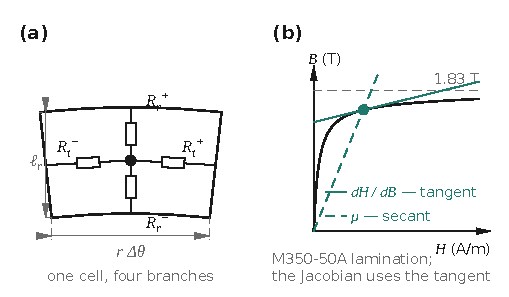
\includegraphics[width=0.86\linewidth]{fig_cell.pdf}
\caption{The four-branch cell and the material law it is solved with.
\textbf{(a)} One cell, with its two radial and two tangential
reluctances meeting at a centre node. \textbf{(b)} The magnetisation
curve of the M350-50A lamination, showing the two slopes a nonlinear
solve may use: the secant $\mu$ and the tangent
$\mathrm{d}H/\mathrm{d}B$, the latter being the one the Jacobian is
built on. Each cell of the polar mesh carries two
radial and two tangential reluctances meeting at its centre node. For an
iron branch $\Delta u = H(B)\ell$ with $B=\Phi/A$, inverted in closed
form by \eqref{eq:branch_inv}, and the Jacobian uses the differential
reluctance $\mathcal{R}_{\mathrm{d}}=(\ell/A)\,\mathrm{d}H/\mathrm{d}B$.
The tangential branches are what allow slot leakage and the depth
grading $h/3b$ of the classical formula to emerge instead of being
added.}
\label{fig:cell}
\end{figure}

\begin{figure*}[!tb]
\centering
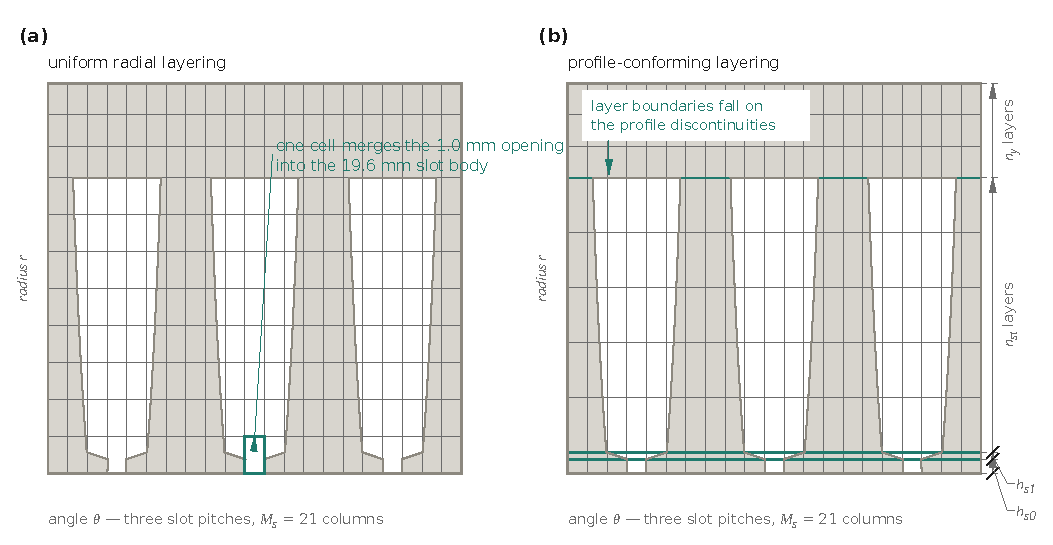
\includegraphics[width=\textwidth,height=0.44\textheight,keepaspectratio]{fig_mesh.pdf}
\caption{Radial layering of the stator mesh, developed along the bore
over three slot pitches. \textbf{(a)} Uniform layering, in which a
single cell is forced to merge the \SI{1.0}{\milli\metre} opening into
the \SI{19.6}{\milli\metre} slot body. \textbf{(b)} The
profile-conforming layering adopted here, whose layer boundaries fall on
the discontinuities of the profile. Both panels carry the same
$M_{\mathrm{s}}=21$ angular columns and differ only in the radial
placement.
Layer boundaries are placed on the discontinuities of the slot profile,
not distributed uniformly: $n_{\mathrm{sh}}$ layers span the opening
$h_{s0}$ and the wedge $h_{s1}$, $n_{\mathrm{st}}$ the slot body
$h_{s2}$, $n_{\mathrm{y}}$ the yoke. Iron and air are assigned per cell
from the true profile, so the tooth width is a solved geometric quantity
rather than an arc subtraction.}
\label{fig:mesh}
\end{figure*}


The iron/air classification within a layer follows the true profile. For
the parallel-sided teeth of the test machine the half-angle of iron at
radius $r$ is $\arcsin\!\big(w_{\mathrm{t}}/2r\big)$ in the slot body
and $\tau_{\mathrm{s}}/2-\arcsin\!\big(w_{\mathrm{o}}/2r\big)$ in the
shoe. Substituting the chord width of the slot directly from the pitch
arc, an approximation that appears natural, yields a tooth of
\SI{4.0}{\milli\metre} instead of \SI{8.49}{\milli\metre} at the slot
bottom, and degrades the fundamental air-gap flux density by
\SI{19}{\percent}.

The angular grid is uniform. The Fourier projection \eqref{eq:W} is
written for surface segments of arbitrary width, but a uniform bore
discretisation keeps the operator well conditioned and lets
\eqref{eq:Ymat} be assembled once.

\subsection{Static Condensation of the Surface Unknowns}
\label{sub:schur}

The surface nodes carry a dense $M_{\mathrm{s}}\times M_{\mathrm{s}}$
block through $\bm{Y}$, whereas the interior blocks are sparse and are
the only ones affected by saturation. Partitioning the nodal system into
surface (s), tooth (t) and yoke (y) unknowns and eliminating the surface
gives
\begin{equation}
\left(\bm{A}_{\mathrm{tt}}
- \bm{A}_{\mathrm{ts}}\bm{A}_{\mathrm{ss}}^{-1}\bm{A}_{\mathrm{st}}\right)
\bm{U}_{\mathrm{t}} + \bm{A}_{\mathrm{ty}}\bm{U}_{\mathrm{y}}
= \bm{r}_{\mathrm{t}}
- \bm{A}_{\mathrm{ts}}\bm{A}_{\mathrm{ss}}^{-1}\bm{i}_{\mathrm{src}} ,
\label{eq:schur}
\end{equation}
in which $\bm{A}_{\mathrm{ss}}$ and $\bm{A}_{\mathrm{st}}$ are invariant
provided the branches touching the surface carry a fixed permeability.

That proviso deserves a direct answer rather than a caveat, because the
tooth tip is precisely where $\mu_{\mathrm{r}}$ swings hardest, between
\num{6727} and \num{9} from one iteration to the next on this machine.
The answer is that the surface block never touches a nonlinear branch.
The nodes carrying $\bm{A}_{\mathrm{ss}}$ lie on the bore, and what
closes on them is the annulus operator: two \emph{linear} media, air and
a magnet whose recoil characteristic is straight to within
\SI{0.24}{\percent} over the working range. The nonlinearity lives one
layer inside, in the iron branches of the shoe cells, and those are
reassembled at every Newton iteration. Freezing $\bm{A}_{\mathrm{ss}}$
is therefore not an approximation whose error must be bounded; it is
exact, and the Schur complement \eqref{eq:schur} may be formed once per
machine without qualification. The Schur
complement is therefore formed once per machine, and each nonlinear
iteration costs only a $2N_{\mathrm{s}}\times 2N_{\mathrm{s}}$ solve.
This is what makes a nonlinear flux map over a
$(\theta,i_\alpha,i_\beta)$ grid, several thousand nonlinear
solutions, affordable.

\subsection{Newton--Raphson Scheme with Differential Reluctance}
\label{sub:newton}

Fig.~\ref{fig:chain} summarises the complete solution chain. Newton
iteration on a reluctance network is established
practice~\cite{tavana2016}; what follows differs only in that the
Jacobian is available in closed form, for the reason given below. The
nonlinear branch obeys $\Delta u = H(B)\,\ell$ with $B=\Phi/A$. Because
the material characteristic supplies $B(H)$, the relation inverts in
closed form,
\begin{equation}
B = B\!\left(\frac{\Delta u}{\ell}\right),
\qquad
\Phi = A\,B ,
\label{eq:branch_inv}
\end{equation}
so the nodal residual is evaluated without any inner iteration. The
Jacobian uses the \emph{differential} permeance
\begin{equation}
G_{\mathrm{d}} = \frac{A}{\ell}\,\left(\frac{\mathrm{d}H}{\mathrm{d}B}
\right)^{\!-1} ,
\label{eq:Gdiff}
\end{equation}
assembled exactly as the linear conductances, with $-\bm{Y}$ added on
the surface block. A backtracking line search protects the first step,
which may otherwise leave the tabulated range of $B(H)$.

\begin{figure}[!ht]
\centering
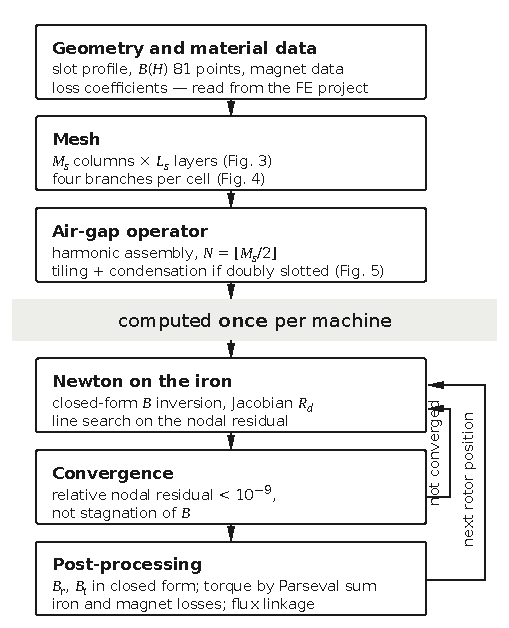
\includegraphics[width=0.95\linewidth]{fig_chain.pdf}
\caption{Solution chain. The shaded step separates what is computed once
per machine from what is repeated: the operator and, where the annulus
has one smooth boundary, its factorisation are reused at every rotor
position, so a sweep of $N_\phi$ positions costs one factorisation and
$N_\phi$ back-substitutions. Newton is warm-started on the previous
position, which reduces the cost to two or three iterations after the
first.}
\label{fig:chain}
\end{figure}

Convergence is measured on the \emph{relative} nodal residual,
$\varepsilon = \|\bm{f}^{(k)}\|/\|\bm{f}^{(0)}\|$, and not on the
stagnation of $B$ or of $\mu_{\mathrm{r}}$, which is the criterion
commonly reported in the MEC literature and which cannot distinguish
convergence from an arrested iteration. The tolerance is
$\varepsilon<10^{-9}$ with a limit of thirty iterations.

Newton iteration has been applied to nonlinear magnetic equivalent
circuits before~\cite{jung2023}; what is added here is that the branch
relation is inverted in closed form, so that no inner iteration is
needed, and that the Jacobian is the differential reluctance itself
rather than a numerical derivative. Table~\ref{tab:newton} contrasts
this scheme with the successive-substitution iteration on
$\mu_{\mathrm{r}}$ that is standard in much of the MEC literature. The
fixed point oscillates because the shoe cells swing between
$\mu_{\mathrm{r}}=6727$ and $\mu_{\mathrm{r}}=9$ from one iteration to
the next; damping it enough to converge requires several hundred
iterations. Newton reaches machine precision in nine. Crucially, the
computed torque is invariant over six decades of tolerance, which
establishes that every result reported below is a converged solution of
the discrete problem and not an artefact of an arrested iteration. This
invariance is not restated at each subsequent use.

\begin{table}[!ht]
\centering
\footnotesize
\begin{tabular}{lcc}
\toprule
Scheme & Iterations & Relative residual \\
\midrule
Successive substitution on $\mu_{\mathrm{r}}$ & 500 & $6.9\times10^{-4}$ \\
Newton, differential reluctance & 9--15 & $5\times10^{-13}$ \\
\bottomrule
\end{tabular}
\caption{Nonlinear solver, PMSM. Tightening the Newton tolerance from
$10^{-6}$ to $10^{-12}$ leaves both the iteration count and the computed
torque unchanged, $\Delta T<\SI{1e-4}{\milli\newton\metre}$.}
\label{tab:newton}
\end{table}


\subsection{Mesh Convergence Study and the Non-Convergent Quantity}
\label{sub:conv}

Tables~\ref{tab:conva} and~\ref{tab:convb} report the behaviour of the
model under the two independent refinements of the stator mesh. They
must be read as a pair, because the two panels move the same quantity in
opposite directions, and that opposition carries the argument of
Section~\ref{sec:bounds}.

\begin{table*}[!t]
\centering
\begin{threeparttable}
\footnotesize
\begin{tabular}{rrrrrr}
\toprule
$M_{\mathrm{s}}$ & unknowns & $\nu=8$ linear & $\nu=8$ Newton
& peak $B$ linear & peak $B$ Newton\\
\midrule
360 & \num{5760}  & $-26.8\%$ & $+10.3\%$ & \SI{2.908}{\tesla} & \SI{1.928}{\tesla}\\
540 & \num{8640}  & $-21.6\%$ & $+15.0\%$ & \SI{3.191}{\tesla} & \SI{1.979}{\tesla}\\
900 & \num{14400} & $-18.8\%$ & $+23.8\%$ & \SI{3.471}{\tesla} & \SI{2.013}{\tesla}\\
\bottomrule
\end{tabular}
\begin{tablenotes}[flushleft]\footnotesize
\item Same machine and reference as Table~\ref{tab:conva};
$n_{\mathrm{sh}}=4$ layers per shoe sub-region (fifteen radial layers),
$n_{\mathrm{st}}=4$, $n_{\mathrm{y}}=3$. The bracket of
Section~\ref{sub:corner} is formed from the $M_{\mathrm{s}}=900$ row of
this same execution.
\item The shoe layering was identified rather than assumed: sweeping
$n_{\mathrm{sh}}$ from 1 to 4 against the six published cells leaves a
maximum residual of \num{9.08}, \num{2.78}, \num{0.81} and \num{0.06}
percentage points respectively. Only $n_{\mathrm{sh}}=4$ reproduces
them.
\end{tablenotes}
\end{threeparttable}
\caption{Radial refinement of the shoe, both solvers on identical
meshes. The linear peak field grows without settling; the Newton peak
field is bounded by saturation but the sideband still moves.}
\label{tab:convb}
\end{table*}

\begin{table*}[!t]
\centering
\begin{threeparttable}
\footnotesize
\begin{tabular}{rrrrrr}
\toprule
$M_{\mathrm{s}}$ & unknowns & $B_{g1}$ & $L_{\mathrm{d}}$ & $\nu=8$
& peak iron $B$\\
\midrule
180 & \num{1800} & $+0.9\%$ & $+0.5\%$ & $-42.3\%$ & \SI{2.209}{\tesla}\\
360 & \num{3600} & $+0.4\%$ & $+0.2\%$ & $-19.8\%$ & \SI{2.570}{\tesla}\\
540 & \num{5400} & $+0.3\%$ & $+0.1\%$ & $-13.3\%$ & \SI{2.699}{\tesla}\\
900 & \num{9000} & $+0.2\%$ & $+2.5\%$ & $-9.7\%$  & \SI{2.799}{\tesla}\\
\bottomrule
\end{tabular}
\begin{tablenotes}[flushleft]\footnotesize
\item PMSM 15/14, $n_{\mathrm{sh}}=1$ layer per shoe sub-region (nine radial
layers), linear solver at $\mu_{\mathrm{r}}=\num{3000}$,
$k_{\mathrm{f}}=\num{0.325}$ (inert in this chain, Section~\ref{sub:fitted}), basis of Section~\ref{sec:trace}
piecewise constant, rotor at $\phi=0$. Deviations against the
finite-element reference $B_{g1}=\SI{1.074548}{\tesla}$,
$\nu=8$ at \SI{0.0196594}{\tesla},
$L_{\mathrm{d}}=\SI{52.3415}{\milli\henry}$. The peak field is that of
the linear solution and is reported to be read against
Table~\ref{tab:convb}.
\end{tablenotes}
\end{threeparttable}
\caption{Angular mesh convergence at one layer per shoe sub-region.
The fundamental converges; the first slot sideband does not, and neither
does the synchronous inductance, for the reason given in the text.}
\label{tab:conva}
\end{table*}

Table~\ref{tab:conva} refines the bore \emph{angularly} at one layer per
shoe sub-region. The radial layering is identical at all four points, nine layers, ten node rows, so this is a pure angular refinement and
may be read as such. The fundamental air-gap flux density converges
monotonically, from \SI{+0.9}{\percent} to \SI{+0.2}{\percent}, and is
settled by $M_{\mathrm{s}}=540$. The synchronous inductance improves in
the same way as far as $M_{\mathrm{s}}=540$, reaching
\SI{+0.1}{\percent}, and then moves to \SI{+2.5}{\percent} at the finest
grid, a reversal of a factor of twenty-five. The movement is carried by
the phase self-inductance itself, which rises from \SI{50.379}{\milli\henry}
to \SI{51.549}{\milli\henry} between the last two grids against a
reference of \SI{50.209}{\milli\henry}, and not by the subtraction that
forms $L_{\mathrm{d}}$ from $L_{\mathrm{a}}$ and $M$; it survives a second
shoe layer, at \SI{+2.0}{\percent}, so it is a property of the angular
tiling. The quantity is therefore not converged over the range examined,
and the deviation quoted for it in Section~\ref{sub:field} and in the
abstract is its value in the configuration declared for
Table~\ref{tab:pmsm} rather than the limit of this sequence.

The first slot sideband $\nu=|N_{\mathrm{s}}-p|=8$ does not converge,
and the table shows why rather than merely asserting it. Refining
angularly \emph{raises} it, from \SI{-42.3}{\percent} to
\SI{-9.7}{\percent}. Refining the shoe radially at fixed angular grid
\emph{lowers} it: at $M_{\mathrm{s}}=900$ the same quantity falls from
\SI{-9.7}{\percent} at one shoe layer to \SI{-18.8}{\percent} at four.
Neither direction approaches the other.

Table~\ref{tab:convb} adds the decisive column. \emph{Three sweeps of
the peak iron flux density are quoted in this paper and they are not the
same experiment}; all three come from the single execution that produced
Table~\ref{tab:convb}, and each is named where it appears. Refining the
\emph{shoe} at $M_{\mathrm{s}}=900$, $n_{\mathrm{sh}}$ from one to
four, the linear solver gives a peak that is not merely high but
\emph{unbounded}, growing from \SI{2.80}{\tesla} to \SI{3.47}{\tesla} on
a material that saturates near \SI{2}{\tesla}, while the Newton solution
on the same meshes is bounded, \SI{2.006}{\tesla} to \SI{2.013}{\tesla},
a drift of \SI{0.34}{\percent}, because saturation constrains it. The
same shoe sweep at $M_{\mathrm{s}}=540$ gives \SI{1.974}{\tesla} to
\SI{1.979}{\tesla} under Newton, and it is that pair which
Section~\ref{sub:integral} quotes. The \emph{angular} sweep at
$n_{\mathrm{sh}}=4$, $M_{\mathrm{s}}$ from 360 to 900, is the Newton
column of Table~\ref{tab:convb} itself, \SI{1.928}{\tesla} to
\SI{2.013}{\tesla}. Reading any one of the three as the others is what
the three-way discrepancy in earlier versions of this manuscript
amounted to. This is worth stating precisely, since it is easy to
misread as a convergence result: \emph{saturation bounds the amplitude
of the field at the corner, not its dependence on the mesh}. The
sideband it drives still moves, and it moves in opposite senses under
the two solvers, the linear solution falls away from the reference, the
Newton solution rises past it.

The consequence is a bracket rather than a value. Its width, measured at
$M_{\mathrm{s}}=900$ between the linear and Newton predictions, is
\num{41.7} points at one shoe layer and \num{42.6} points at four: the
bracket does not close under refinement of the very region that is
supposed to resolve it. A quantity whose refined value depends on the
direction of refinement, bracketed by two solvers whose separation does
not shrink, and accompanied in one of them by a field that grows without
bound, is not under-resolved. It is singular, and
Section~\ref{sec:bounds} identifies the singularity and shows that it is
present in the finite-element reference as well.



\subsection{Elimination of Empirically Fitted Constants}
\label{sub:fitted}
In the lumped counterpart of this network, one branch per tooth and per
yoke segment, the slot-opening fringing is carried by a constant
$k_{\mathrm{f}}$ identified on finite-element field profiles, the slot
leakage is added analytically as a trapezoidal permeance, and a
tooth-tip leakage term $\lambda_{\mathrm{tip}}$ must be cancelled in the
armature problem to avoid double counting. Three conventions, all
documented but all fragile.

The mesh removes them. The opening, the wedge and the tangential leakage
paths are resolved explicitly, so no fringing constant is required; the
slot leakage is carried by the air cells of the slot, so no analytical
permeance is added; and the depth grading of the leakage, the $h/(3b)$
of the classical formula, \emph{emerges} from the network, since the
flux must come from the tooth to cross the slot at each depth.
Section~\ref{sec:pmsm} shows that the inductances so obtained are more
accurate than those of the fitted lumped model.

The claim is worth attaching to a number rather than left as an
argument. On the refined mesh the phase self-inductance, the quantity
that carries the slot leakage, is high by \SI{0.34}{\percent} against
the finite-element reference, where the lumped model with its three
conventions is high by \SI{1.12}{\percent}. The leakage the mesh
resolves is therefore not merely obtained without a constant; it is
obtained better than with one.

\paragraph{The fringing coefficient, and why it is absent rather than
merely unused.}
The first of the three constants deserves to be followed through,
because it is the one that is genuinely an \emph{air-gap} parameter and
because the tables of Section~\ref{sec:pmsm} still declare a value for
it. In the lumped network the flux entering radially through the slot
mouth has no path of its own, so it is carried by a single conductance
$G_{\mathrm{fr}}=k_{\mathrm{f}}\,\mu_0(\Delta\theta R_{\mathrm{s}})L/(b_0/2)$
placed across the opening. The mesh resolves that entry explicitly, the
isthmus and bevel layers, and the tangential leakage branches between
them, so the same conductance is \emph{not} assembled there: adding it
would count one fringing path twice. The parameter is therefore carried
through the mesh chain as a declared configuration field and used by no
permeance, which a numerical control confirms: changing it from
\num{0.325} to \num{0.750} leaves the computed slot sideband identical
to twelve significant figures. It is reported in the table notes because
it parameterises the lumped column, and for no other reason.

Two identifications of the same constant, on the same machine, illustrate
what is being removed. Fitted against the finite-element tooth-band
amplitudes it comes out at \num{0.75}; fitted against the three lumped
field quantities of Section~\ref{sub:field} it comes out at
\num{0.325}, a factor of \num{2.3} apart, each defensible on its own
bench. A coefficient whose value depends on which quantity it is
identified against is not a property of the geometry, and that, rather
than the count of constants, is what the operator removes.

One reservation attaches to the synchronous inductance and is stated
where the table appears rather than here, because it concerns the way
two errors combine in $L_{\mathrm{d}}=L_a-M$ and not the removal of the
constants themselves; see Section~\ref{sub:field}.

\subsection{Computational Cost and Scaling}
\label{sub:compcost}

The economy of a reduced-order model is its reason for existing and is
therefore stated explicitly rather than assumed. One figure is reported,
and one comparison is deliberately not.

The complete study of this machine, eight analyses, from the no-load
field to the speed sweep, comprising twenty-nine compared quantities and
nine figures, executes in \SI{133}{\second} on a desktop workstation,
the refined network carrying \num{10800} unknowns.

The structural reason is \eqref{eq:schur} together with the position
invariance of Section~\ref{sub:props}. A rotor sweep of $N_\phi$
positions costs one assembly and one factorisation of the dense surface
block, then $N_\phi$ back-substitutions on a system the size of the
tooth set; Newton, warm-started on the previous position, needs two or
three iterations after the first. One figure makes the scale concrete:
the coupled network is solved at \num{721} rotor positions on \num{1260}
surface nodes in \SI{3}{\second}, the entire no-load angular sweep on
which the field, the flux linkage, the electromotive force and the
cogging torque are built. That number is what makes a cogging
computation a routine step rather than a study of its own, and it exists
only because the annulus does not move relative to the stator. Where
both bounding surfaces are slotted the coupling block must be rebuilt at
every position.

What is \emph{not} reported is a wall-clock ratio against the
finite-element reference, and the reason is worth giving because such
ratios are reported routinely. The reference runs available here were
executed on different hardware, at a different date, and under a
meshing and time-step policy chosen separately for each study; their
recorded times cover parametric sweeps whose scope is not that of the
present study. A ratio drawn from them would measure two unrelated
configurations rather than two methods, and would flatter this one. A
controlled comparison, both methods on the same machine, to a common
accuracy target on a named quantity, is the proper form of that claim,
and it is left to further work instead of approximated here.


%======================================================================

%=======================================================================
%  ARTICLE I -- SECTION 5 : PROTOCOLE DE VALIDATION
%
%  Restructuration en huit rubriques qui remplissent, une a une, les
%  FONCTIONS de la liste PRISMA 2020 demandee -- protocole, criteres
%  d'admissibilite, sources, strategie de localisation, selection,
%  extraction, risque de biais, analyse -- transposees a une etude
%  numerique.  Aucun enregistrement PROSPERO n'est invente ; aucun I2,
%  Q de Cochran, funnel plot ni test d'Egger n'est calcule, et le §5.8
%  dit pourquoi.
%
%  Prose continue : les deux listes enumerate de l'ancienne version
%  (protocole de mesure, quatre verifications internes) sont passees en
%  prose.
%
%  Labels conserves parce que reference ailleurs : sec:methods,
%  sub:posture, sub:provenance, sub:align, fig:protocol, tab:machines,
%  eq:eta.
%
%  CHIFFRES NOUVEAUX, TOUS TRACABLES :
%                          dans MEC_BLDC et MEC_IM (7 aout 2026).
%=======================================================================
\section{Validation Protocol}
\label{sec:methods}

The protocol is reported at the length usually reserved for a review of
evidence, and for the same reason: what separates a formulation claim
from a coincidence is not the size of the agreement but the discipline
with which the comparison was fixed, the provenance of every number
admitted to it, and the completeness of what is reported afterwards.

\subsection{Pre-Specified Protocol and Fixed Parameters}
\label{sub:protocol}

There is no public registry for computational studies of this kind and
none is claimed. What is used instead is a versioned manifest, kept in
the same repository as the code, which names for every published
quantity the chain that produces it, the output file it is read from,
the date of that output, and the configuration that defines it. Its
purpose is the purpose of a registration: to prevent the analysis plan
from being selected after the results are known. Its limitation is
stated with equal clarity. The manifest was written after the runs had
been executed and before the tables were filled, so it fixes the
extraction and reporting plan but not the run plan; it is weaker than a
pre-registration and is not offered as one.

Five rules govern it. No value is transcribed by hand: every number in
this paper is read from a dated output at full precision, and every
deviation is formed on the full-precision values and rounded once, at
display. Every table declares its configuration, machine, angular
columns $M_{\mathrm{s}}$, radial layers $n_{\mathrm{sh}}$, surface
basis, solver, and the reference study used. One quantity is produced by
one declared chain, so that where two implementations compute the same
thing only one is authoritative. A result that cannot be regenerated is
withdrawn rather than kept with a note. And a discrepancy is never
reconciled by changing the reference.

Two deviations from the protocol occurred and are recorded rather than
silently absorbed. The extraction rule was first written as ``the second
block of an output file is authoritative''; that formulation is false on
at least one file and was replaced by the rule of
Section~\ref{sub:extraction}. And one convergence panel was normalised
against half the predicted slope instead of the slope itself, which
made a verified asymptote appear to be missed by a factor of two; the
figure was recomputed, and the closed form of Section~\ref{sec:trace}
was unaffected.

\subsection{Admissibility Criteria for Reported Quantities}
\label{sub:eligibility}

The comparison is specified before it is made, in the four terms a
clinical protocol would call population, intervention, comparator and
outcome, because those four are precisely what a numerical validation
gets wrong when it goes wrong.

The population is a single machine in a declared state. Its geometry,
its winding and its materials enter the model by direct read of the
finite-element project, never by transcription, and the declaration
extends past the hardware to the numerical state: the angular columns and radial layers of the
mesh, the surface basis, the harmonic truncation and the solver
tolerance are part of the specimen, not of the method. The intervention
is the air-gap closure, and it is the only thing allowed to vary along a
given axis of comparison. The comparator is a named finite-element
study, not the project, the study, because a project of this kind
produces the same physical quantity by several routes that do not carry
the same numerical resolution. The outcome is a functional, defined
identically on both sides and evaluated at the same location.

A quantity is admitted to a table when three conditions hold together:
it is produced by a declared chain from a dated output; it is defined by
the same functional in both models; and the determination used on the
reference side is named. Two classes are excluded by construction. A
quantity for which the reference offers several determinations without
one being nominated is not reported, because quoting whichever is closer
converts a provenance question into a modelling result. And a quantity
whose value depends on a constant identified against the same reference
is not reported as a validation of that reference, because the
comparison would be circular; Section~\ref{sub:fitted} states which
constants remain identified and where their influence lies.

The consequence for the design of the comparison is that two axes are
used and kept separate throughout (Fig.~\ref{fig:protocol}). Along the
\emph{iron} axis the closure is held fixed at the DtN operator while the
iron discretisation is varied between the refined polar mesh and its
one-branch-per-tooth counterpart; this is Table~\ref{tab:pmsm}. Along
the \emph{closure} axis the iron model is held fixed at the lumped
network while the closure is varied between Carter's factor, a permeance
function and the operator; this is Table~\ref{tab:carter}. Varying both
at once would make any improvement unattributable.

\begin{table*}[!t]
\centering
\begin{threeparttable}
\footnotesize
\begin{tabular}{@{}lrrrr@{}}
\toprule
Quantity & Mesh $n_{\mathrm{sh}}{=}1$ & Mesh $n_{\mathrm{sh}}{=}2$
& Lumped & FEA\\
\midrule
$B_{g1}$ (T)                          & 1.07787 & 1.07908 & 1.07755 & 1.07455\\
$|B_r|$ mean (T)                      & 0.76182 & 0.76273 & 0.76147 & 0.76091\\
$B_r$ peak (T)                        & 0.98051 & 0.97536 & 0.98600 & 0.99073\\
$B_t$ rms (T)                         & 0.13755 & 0.13478 & 0.14317 & 0.13326\\
slot sideband $\nu=8$ (T)             & 0.01704 & 0.01581 & 0.01806 & 0.01966\\
flux line $A$ (Wb/m)                  & 0.00586 & 0.00587 & 0.00586 & 0.00585\\
flux linkage, peak (Wb)               & 0.25894 & 0.25908 & 0.26121 & 0.25833\\
MMF per magnet (A)                    & 761.674 & 759.329 & 762.912 & 769.445\\
MMF per gap (A)                       & 711.386 & 711.880 & 725.064 & 721.504\\
MMF dispersion (\%)                   & 6.369   & 5.959   & 6.810   & 6.585\\
phase back-EMF, peak (V)              & 238.813 & 238.818 & 240.877 & 233.031\\
six-step envelope (V)                 & 464.556 & 464.645 & 468.719 & 459.918\\
$L_{\mathrm{a}}$ (mH)                 & 50.379  & 50.484  & 50.773  & 50.209\\
$M$ (mH)                              & $-2.016$& $-2.021$& $-2.220$& $-2.133$\\
$L_{\mathrm{d}}$ (mH)                 & 52.395  & 52.505  & 52.993  & 52.342\\
$k_{\mathrm{r}}$                      & 1.07069 & 1.06665 & 1.05220 & 1.08693\\
$k_{\mathrm{l}}$                      & 0.85326 & 0.85368 & 0.85371 & 0.86723\\
\midrule
\multicolumn{5}{l}{\emph{deviation from the reference, formed on the full-precision values}}\\
$B_{g1}$                              & $+0.31\%$ & $+0.42\%$ & $+0.28\%$ &, \\
$|B_r|$ mean                          & $+0.12\%$ & $+0.24\%$ & $+0.07\%$ &, \\
$B_r$ peak                            & $-1.03\%$ & $-1.55\%$ & $-0.48\%$ &, \\
$B_t$ rms                             & $+3.22\%$ & $+1.14\%$ & $+7.43\%$ &, \\
slot sideband $\nu=8$                 & $-13.34\%$& $-19.58\%$& $-8.12\%$ &, \\
flux line $A$                         & $+0.12\%$ & $+0.22\%$ & $+0.09\%$ &, \\
flux linkage, peak                    & $+0.24\%$ & $+0.29\%$ & $+1.11\%$ &, \\
MMF per magnet                        & $-1.01\%$ & $-1.32\%$ & $-0.85\%$ &, \\
MMF per gap                           & $-1.40\%$ & $-1.33\%$ & $+0.49\%$ &, \\
MMF dispersion                        & $-3.27\%$ & $-9.50\%$ & $+3.42\%$ &, \\
phase back-EMF, peak                  & $+2.48\%$ & $+2.48\%$ & $+3.37\%$ &, \\
six-step envelope                     & $+1.01\%$ & $+1.03\%$ & $+1.91\%$ &, \\
$L_{\mathrm{a}}$                      & $+0.34\%$ & $+0.55\%$ & $+1.12\%$ &, \\
$M$                                   & $-5.48\%$ & $-5.24\%$ & $+4.09\%$ &, \\
$L_{\mathrm{d}}$                      & $+0.10\%$ & $+0.31\%$ & $+1.24\%$ &, \\
$k_{\mathrm{r}}$                      & $-1.49\%$ & $-1.87\%$ & $-3.20\%$ &, \\
$k_{\mathrm{l}}$                      & $-1.61\%$ & $-1.56\%$ & $-1.56\%$ & ---\\
\bottomrule
\end{tabular}
\begin{tablenotes}[flushleft]\footnotesize
\item PMSM 15/14, $M_{\mathrm{s}}=540$, $N_p=61$ rotor positions,
piecewise-constant surface basis, $k_{\mathrm{f}}=\num{0.325}$ (inert in the mesh columns, Section~\ref{sub:fitted}),
\emph{linear solver at $\mu_{\mathrm{r}}=\num{3000}$ throughout}.
Unknowns: \num{5400} at $n_{\mathrm{sh}}=1$, \num{6480} at
$n_{\mathrm{sh}}=2$, \num{1260} surface columns for the lumped network.
Reference values read from the finite-element project, none transcribed.
Deviations are formed on the full-precision values; two of them, the
mutuals, move by \num{0.32} and \num{0.14} percentage points if formed
on the rounded millihenries printed above, which is why the rule is
stated.
\item $k_{\mathrm{r}}$ is computed retaining the outlying gap
magnetomotive force (MMF) discussed in Section~\ref{sub:kr}. Excluding it
gives a second reference, \num{1.0664}. All four deviations are given
together so that no column is shown against the reference that favours
it: against \num{1.0869} they are \SI{-1.49}{\percent} at one shoe layer,
\SI{-1.87}{\percent} at two and \SI{-3.20}{\percent} on the lumped
column; against \num{1.0664} they are \SI{+0.40}{\percent},
\SI{+0.02}{\percent} and \SI{-1.34}{\percent}. The factor is reported
with both determinations and no selection between them is made.
\end{tablenotes}
\end{threeparttable}
\caption{PMSM at no load: the mesh model at two shoe layerings, its
lumped counterpart, and the two-dimensional finite-element reference.
All four columns carry the same DtN operator on the bore and differ only
in the iron.}
\label{tab:pmsm}
\end{table*}

\begin{figure}[!ht]
\centering
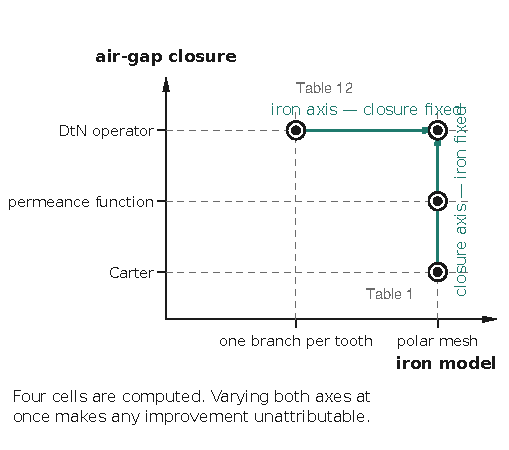
\includegraphics[width=0.9\linewidth]{fig_protocol.pdf}
\caption{The two comparison axes, kept separate throughout. Along the
iron axis the air-gap closure is held at the DtN operator and the iron
discretisation is varied (Table~\ref{tab:pmsm}); along the closure axis
the iron is held at the lumped network and the closure is varied
(Table~\ref{tab:carter}). All figures and tables of
Section~\ref{sec:pmsm} other than Table~\ref{tab:pmsm} use the lumped
iron model. Varying both at once would make any
improvement unattributable.}
\label{fig:protocol}
\end{figure}

\subsection{Information Sources and Reference Data}
\label{sub:provenance}

Three classes of source feed this paper and no others. The first is the
finite-element project itself, from which the geometry, the winding, the
lamination characteristic, the magnet data and the loss coefficients are
read directly. The second is the set of solved reference studies: a
magnetostatic study, a transient no-load study, a transient on-load
study and a speed sweep at constant dc-bus voltage, each a separate
solution and each named where it is used. The third is the set of dated
transcripts written by the network runs themselves, which are the only
route by which a computed number reaches a table.

The reference is ANSYS Maxwell 2-D. No parameter is adjusted and no
intermediate value is transcribed by hand, so that the two models are
guaranteed to solve the same problem. The lamination characteristic is
the measured 81-point $B(H)$ curve of the M350-50A steel, taken verbatim
from the material definition of the project and assigned to both stator
and rotor. The magnet is described by its remanence of
\SI{1.2471}{\tesla} and coercivity of \SI{955}{\kilo\ampere\per\metre},
from which the recoil permeability
$\murec = B_{\mathrm{r}}/(\mu_0 H_{\mathrm{c}}) = 1.0390$ follows,
together with a resistivity of \SI{1.80e-6}{\ohm\metre}. Iron losses use
the Bertotti coefficients of the reference itself~\cite{bertotti},
$k_{\mathrm{h}} = 182.455$, $k_{\mathrm{c}} = 1.34676$ and
$k_{\mathrm{e}} = 0$, the eddy-current term being formed on the time
derivative of the flux density throughout, the amplitude form being used
only where it is named, with a mass density of
\SI{7650}{\kilogram\per\metre\cubed} and a stacking factor of 0.90.
Table~\ref{tab:machines} lists the geometry, winding and material data,
every entry read from the project rather than transcribed.

\begin{table}[!ht]
\centering
\begin{threeparttable}
\footnotesize
\begin{tabular}{@{}lr@{}}
\toprule
 & PMSM 15/14 \\
\midrule
rated output & \SI{750}{\watt} \\
slots / poles & 15 / 14 ($p=7$) \\
stator bore $D$ (mm) & 69.356 \\
stator outer diameter (mm) & 125.0 \\
mechanical air gap $g$ (mm) & 1.000 \\
active length $L$ (mm) & 33.0 \\
magnet thickness (mm) & 3.500 (embrace 0.94) \\
tooth width (mm) & 8.490 \\
slot height $h_{s0}/h_{s1}/h_{s2}$ (mm) & 1.00 / 0.50 / 19.60\tnote{a} \\
slot width $b_{s0}/b_{s1}/b_{s2}$ (mm) & 2.00 / 6.70 / 15.03 \\
total slot height (mm) & 21.10 \\
stator / rotor yoke (mm) & 6.722 / 14.678 \\
\midrule
winding factor $k_{w1}$ & 0.9514 \\
turns per coil / per phase & 152 / 760 \\
winding layers / parallel paths & 1 / 1 \\
phase resistance ($\Omega$) & 10.220 \\
lamination & M350-50A \\
stacking factor & 0.90 \\
Bertotti $k_{\mathrm{h}}$, $k_{\mathrm{c}}$, $k_{\mathrm{e}}$ & 182.455, 1.34676, 0\tnote{b} \\
magnet & N42UH \\
\quad $B_{\mathrm{r}}$ (T) / $H_{\mathrm{c}}$ (kA/m) & 1.2471 / 955 \\
\quad $\murec$ / $\sigma$ (S/m) & 1.0390 / \num{555556} \\
supply & \SI{500}{\volt} dc, six-step \\
\midrule
moment of inertia (kg\,m$^2$)\tnote{c} & \num{1.0e-3} \\
viscous damping (N\,m\,s) & \num{6.07927101854027e-4} \\
load torque (N\,m) & 4.8 \\
\bottomrule
\end{tabular}
\begin{tablenotes}[flushleft]\footnotesize
\item[a] Slot type tc6, semi-closed with parallel-sided teeth; the
parallel-tooth condition is satisfied to $1.7\times10^{-6}$ in the
generated profile.
\item[b] The excess-loss coefficient is zero in the project's own
material definition, so the Bertotti separation reduces here to
hysteresis and eddy currents. This is stated rather than reported as a
column of zeros.
\item[c] The three mechanical rows are the reference project's own
motion setup, and the network drive model of
Section~\ref{sub:drive_results} integrates the same three. An earlier
version of this table gave \num{3.789e-4} for the inertia; that figure
came from a dimensioning sheet, not from the project, and it is
inconsistent with both the reference and the model. The rise-time
comparison of Table~\ref{tab:load} rests on this row, which is why it is
given with its two companions instead of alone.
\end{tablenotes}
\end{threeparttable}
\caption{Data of the test machine, read directly from the
finite-element project. Rows above the rule are geometry, below it
winding and materials.}
\label{tab:machines}
\end{table}

Efficiency is evaluated with the exact definition used by the reference,
\begin{equation}
\eta = \frac{P_{\mathrm{out}}}
{1.02\,P_{\mathrm{out}} + P_{\mathrm{cu}}
 + P_{\mathrm{core}} + P_{\mathrm{solid}}},
\label{eq:eta}
\end{equation}
in which the factor 1.02 is the reference's flat-rate allowance for
friction and windage, applied to the shaft power. Two points follow and
are stated because they bound the interpretation of every efficiency
quoted in this paper. First, \eqref{eq:eta} is adopted so that the
network computes the \emph{same functional of the field} as the
reference rather than a nominally similar one; it is a comparison
functional, not a normative efficiency, and it is not the efficiency
defined by IEC~60034-2-1. Second, because the flat-rate term is common
to both columns, it contributes nothing to their difference. The
reluctance and leakage factors likewise follow the project's own
output-variable definitions. The single quantity taken from the
reference is the angular origin relating the two coordinate systems,
established once as described in Section~\ref{sub:align} and applied
unchanged thereafter.

\subsection{Traceability of Reported Values: One Quantity, One Chain}
\label{sub:chain}

The repository holds \num{76} executable run scripts for this machine,
of which \num{18} write a dated transcript. That asymmetry is deliberate
and is the reason a locating rule is needed at all: most of the scripts
are diagnostics, several compute a quantity that is also computed
elsewhere, and nothing in the file system distinguishes an authoritative
chain from an exploratory one. The manifest makes that distinction
explicit, quantity by quantity, and it is the only admissible route from
a number in a table back to the computation that produced it.

Where two chains compute the same quantity, both are kept and one is
declared. They are kept because a diagnostic that contradicts the
declared chain is evidence and deleting it destroys the record; only one
is declared because the alternative, reporting whichever agrees better
with the reference, is the mechanism by which a provenance question
becomes an apparent result. The rule is applied in the direction that
costs something: Section~\ref{sub:selection} gives the case in which the
declared chain is the one that disagrees with a published claim, and the
claim was moved rather than the chain.

\subsection{Selection of Runs and Exclusion Criteria}
\label{sub:selection}

Three exclusions were applied, each for a stated reason, and each is
recorded here rather than left to be inferred from an absence.

The transcript feeding the principal comparison table holds four starts
and three completed runs, and only the last of those is used. In the two
earlier ones the mesh columns return a peak phase electromotive force of
exactly zero, a deviation of \SI{-100}{\percent}, against
\SI{238.81}{\volt} in the run that is retained; the cause is a warm
start on the surface potentials, which is admissible only under the
Newton solver. The broken runs are not deleted, because their failure is
what establishes the extraction rule of
Section~\ref{sub:extraction}, but no number is taken from them.

One chain is excluded although its results are not wrong. A mesh-based
inductance script reproduces the reference self-inductance to a few
tenths of a percent, but the diagnostic it exists to print, the share
of the armature flux carried by the air cells of the slot, and the share
crossing the air-gap surface, is identically zero by construction, both
terms being multiplied by zero in the source. The sentence printed
immediately below those two zeros, asserting that the slot leakage is
resolved by the mesh rather than added as a formula, is therefore
supported by no number in that transcript. The chain was excluded rather
than repaired; that is the point of the rule, and the claim itself
was moved instead of being defended: it rests on the mutual-inductance
chain, where the mesh reproduces the reference self-inductance of
\SI{50.209}{\milli\henry} to \SI{0.34}{\percent} with the slot leakage
carried by the air cells and nothing added
(Section~\ref{sub:fitted}). A claim was moved to a chain that supports
it; no chain was adjusted to support a claim.

One reference point is excluded. The first point of the speed sweep, at
\SI{10}{\rpm}, is not a periodic steady-state average in the reference:
the rotor does not cover one electrical period within the simulation
window, no commutation occurs, and the reported root-mean-square (rms) current
is that of a direct current. Test~5 of Section~\ref{sec:audit}
establishes this. The point is quoted for completeness where the
characteristic is tabulated and excluded from every mean.

Diagnostic runs, including hypotheses that were tested and rejected, are
retained in the repository as separate scripts rather than discarded, so
that the reasoning behind each reported bound can be reconstructed by a
reader who has the code.

\subsection{Extraction, Registration and Definition of the Compared Quantities}
\label{sub:extraction}
\label{sub:align}

A transcript may contain several solved blocks, and the one that is
authoritative is the last \emph{complete} block, complete meaning that
its own internal consistency has been checked, not merely that it comes
last.
Rank alone is not a criterion, which is what the four-block case above
demonstrates. A table is filled from a transcript and never from another
table, so that a transcription error cannot propagate between tables,
and no rounded value is ever used as the input of a further computation.

The network and the reference use different angular origins and, for the
transient studies, different time origins. A single registration is
established per machine and then held fixed for every comparison. It is
established on the \emph{flux linkage} rather than on the
back-electromotive force: the flux linkage is the primary quantity, the
electromotive force is its time derivative, and differentiating
amplifies exactly the high-order content the registration is meant to
align. The offset minimising the root-mean-square difference between the
two flux-linkage waveforms over one electrical period is
\SI{143.49}{\degree} electrical for the PMSM. Applied unchanged, the
residual optimal shift is \SI{-0.5}{\degree}, and the residual
root-mean-square differences are \SI{0.0036}{\weber} on flux linkage and
\SI{6.7}{\volt} on electromotive force, or \SI{1.4}{\percent} and
\SI{2.9}{\percent} of the respective peaks. \emph{These two figures are
reported as results and not merely as a by-product of the registration}:
they are the only waveform-level error measures in this paper, and they
say what a fundamental agreeing to a few tenths of a percent does not, that the curves also agree away from their peaks, to within one and
three percent respectively. A sign convention is also
reconciled: the reference reports $+\mathrm{d}\lambda/\mathrm{d}t$
whereas the network computes $-\omega\,\partial\lambda/\partial\theta$.
The sign is reversed at display only, never in the computation.

Comparisons are then made on identically defined functionals evaluated
at identical locations. Air-gap flux densities are taken at the mid-gap
radius $r = \Rs - g/2$, the probe radius of the reference; torque
follows from \eqref{eq:torque} on a circle inside the air gap; magnet
losses follow \eqref{eq:pmloss}, with the zero-net-current constraint
imposed over the entire magnet cross-section and the time derivative
taken on coefficients already expressed in the rotor frame. Every table
below states the study its reference column comes from, and
Section~\ref{sub:field} states the one case in which two determinations
of the same quantity are reported side by side, because there they are
not the same functional of the field.

\subsection{Bias Assessment of the Reference and Internal Verification}
\label{sub:posture}

The reference carries its own error, and the posture that follows is
stated rather than left implicit: a numerical reference is not a
measurement, so comparing two numerical models bounds their difference
and never their common distance from the physical machine.
Section~\ref{sec:audit} therefore assesses the reference before any
agreement is claimed, using a five-test instrument developed for that
purpose and applicable without re-solving the reference. The instrument
asks whether the reported quantity is a periodic steady-state average,
whether its spectrum contains orders the geometry can physically
support, whether two meshing strategies of the same model agree, whether
the residual after removing the physical content is consistent with mesh
noise, and whether the quantity depends on a solver setting it should
not depend on. On this machine the instrument changed the reading of one
quantity, and the change was unfavourable to the model.

Four checks are applied to the network solution itself, independently of
the reference, so that a discrepancy can be attributed rather than
merely observed. Continuity of the radial flux density across the
magnet/air interface is required and holds to $4.3\times10^{-16}$ over
the orders $n\le80$ that carry the field---beyond that the residual
loses meaning instead of degrading, since $\sinh(n\Um)$ exceeds
$10^{29}$ and the orders concerned transfer nothing, so the relative
check would be formed on quantities that are numerically zero. The
computed torque is invariant when the Newton tolerance is tightened over
six decades (Section~\ref{sub:newton}). The flux conservation of the
solved cross-section closes to $1.5\times10^{-17}$\,Wb, which verifies
the assembly of the network in place of its physics. And wherever a
torque discrepancy is reported, the ratio of the sum of absolute terms
to the algebraic sum of \eqref{eq:torque} is computed, so that a genuine
physical difference can be separated from cancellation in the Parseval
sum.

Experimental confirmation on a prototype remains necessary before the
model is used for absolute performance prediction. It is not required to
establish the formulation claim made here, and \emph{no experimental
agreement is asserted anywhere in this paper}. For completeness the
measurement protocol that would close the gap is specified, since it is
short and unambiguous: two open-circuit quantities suffice, so neither
requires a loaded dynamometer. The first is the phase resistance at a
controlled winding temperature, four-wire, which fixes the only
non-magnetic parameter entering the drive model and removes the
temperature ambiguity from every loss comparison, an ambiguity
Section~\ref{sub:drive_results} shows is not hypothetical. The second is
the open-circuit back-electromotive force, line-to-line, at a measured
shaft speed and recorded over at least one electrical period; that
single waveform tests the whole chain at once, its fundamental testing
the magnetisation spectrum \eqref{eq:Mn} and the transfer $\alpha_n$ of
\eqref{eq:alpha}, its harmonic content testing the slot modulation
carried by $g_n$, and its peak-to-peak envelope being the quantity that
governs the drive operating point. A third measurement, the static
torque--angle curve at a known dc current, would additionally separate
the magnet contribution from the armature reaction; it is desirable but
not necessary. The bounded quantities of Section~\ref{sec:bounds} cannot
be settled by measurement either, since they are governed by a geometric
singularity that the manufactured tooth-tip radius, unknown here, would
itself determine.

\emph{A protocol without an accuracy class is a gesture, not a
specification.} The integral deviations this paper reports lie between
\SI{0.1}{\percent} and \SI{0.35}{\percent}, so a measurement that cannot
resolve a few tenths of a percent cannot test them. The class required
is therefore stated: \SI{\le0.2}{\percent} on the line-to-line
root-mean-square electromotive force, \SI{\le0.1}{\percent} on shaft
speed, and \SI{\le0.5}{\percent} on winding resistance with the winding
temperature itself measured to \SI{\pm2}{\kelvin}.

At that class the measurement would discriminate on flux linkage,
back-electromotive force and the synchronous inductance, whose
deviations exceed the combined uncertainty. It would \emph{not}
discriminate on the mutual inductance taken alone, nor on any quantity
whose deviation is of the order of a few tenths of a percent once the
speed and voltage uncertainties are compounded, and it would say
nothing at all about the slot sidebands or the cogging torque, for the
reason just given. Stating what a measurement could not settle is part
of specifying it.

\subsection{Deviation Metrics, Dispersion, and Scope of the Available Analyses}
\label{sub:stats}

The effect measure is the signed relative deviation
\begin{equation}
\delta = \frac{x_{\mathrm{MEC}}-x_{\mathrm{FEA}}}{x_{\mathrm{FEA}}},
\label{eq:delta}
\end{equation}
formed on full-precision values and rounded once for display. The
\emph{dispersion} of a swept quantity, used in Tables~\ref{tab:p0tail},
\ref{tab:v1basis} and~\ref{tab:pmsm}, is $(\max-\min)/\mathrm{mean}$
over the points of the sweep.
\emph{Two further measures are reported for waveforms}, since a
peak-to-peak or a spectral line does not say how two curves differ point
by point: the root-mean-square of the pointwise difference after
registration, and the maximum pointwise difference, each normalised to
the reference. Section~\ref{sub:extraction} gives them for the two
waveforms on which the whole drive chain rests---\SI{0.0036}{\weber} and
\SI{6.7}{\volt} in absolute terms, \SI{1.4}{\percent} and
\SI{2.9}{\percent} of the respective peaks, and they are results rather
than by-products of the alignment procedure that produced them.
Quantities
that are themselves ratios in percent, efficiency above all, are
compared as a difference in points and marked as such, because a
relative deviation on a percentage is ambiguous. Where a deviation is
signed in the text, the sign is that of \eqref{eq:delta}: negative means
the network is below the reference.

Quantities are reported individually. The single aggregate used anywhere
in this paper is a mean absolute deviation over an explicitly enumerated
set, the twenty-eight sweep points above \SI{100}{\rpm}, and the set is
restated wherever the mean appears. There is no weighting and no
pooling, and this is a substantive choice rather than an omission. A
pooled effect, a random-effects model, $I^{2}$, Cochran's $Q$, a funnel
plot and Egger's test all estimate or test the behaviour of one effect
across a \emph{sample of independent studies}. Here there is one
machine, one reference and one implementation, and the quantities
compared are not replicates of a common effect but different functionals
of the same two field solutions, strongly dependent on one another by
construction: the flux linkage, the electromotive force and the
inductances are related by differentiation and by the same surface
potentials. A heterogeneity statistic computed over such a set would
attach a sampling structure to it that it does not have, and the number
would be reportable but meaningless. None is computed.

What replaces dispersion across studies is dispersion across the
choices that a numerical model actually has, reported as a bracket
rather than as a point wherever the choice matters. Four sensitivity
analyses are carried through the paper. The shoe layering is varied from
$n_{\mathrm{sh}}=1$ to $n_{\mathrm{sh}}=4$ over the identification sweep
(Table~\ref{tab:conva}), and the columns at $n_{\mathrm{sh}}=1$ and
$n_{\mathrm{sh}}=2$ are reported side by side throughout, neither being
nominated as the reference model. The harmonic truncation is swept over four
decades, which is the experiment on which the trace-conformity result of
Section~\ref{sec:trace} rests. The Newton tolerance is tightened over
six decades. And the fringing constant of the lumped counterpart is
varied over the full range spanned by its two independent
identifications and shown to leave the mesh chain unchanged to twelve
significant figures, which is what converts the claim that it is inert
into a measurement (Section~\ref{sub:fitted}).

The analogue of a small-study bias assessment is not a plot but a rule,
and it is the one rule that a reader cannot verify from the outside: the
comparison set is reported in full. The twenty-nine quantities it
contains are the twenty-nine bars of Fig.~\ref{fig:score}, and each one
is tabulated with its model value, its reference value and its deviation
in Table~\ref{tab:scorecard}, so that the synthesis can be audited
line by line rather than read off a plot. The set includes the
quantities on which the operator loses. Two are
visible without searching. A coarser model is closer to the reference
than the operator on the first tooth flux-density band, and
Section~\ref{sub:corner} reports and explains that instead of omitting
the row; and the drive comparison, whose efficiency agreement is the
most quotable number in the paper, is reported together with the
operating point at which it is obtained, which is not the reference's.
Where the paper states a bound instead of a value, it is because the
bracket does not close under refinement, and Section~\ref{sec:bounds}
shows the refinement that fails to close it.

%=======================================================================


\section{Validation: 15-Slot/14-Pole PMSM}
\label{sec:pmsm}

\subsection{The Two Iron Models and the Rationale for Reporting Both}
\label{sub:twomodels}

Two discretisations of the iron are used throughout, and they must not
be conflated. The \emph{mesh} model is the polar network of
Section~\ref{sec:mesh}, $M_{\mathrm{s}}$ angular columns by
$L_{\mathrm{s}}$ radial layers, in which the slot opening, the wedge and
the slot leakage paths are resolved explicitly. The \emph{lumped} model
is its classical counterpart, one branch per tooth and per yoke segment,
which needs the three fitted constants listed in
Section~\ref{sec:mesh}. \emph{Both carry the same DtN operator on the
bore}: they differ only in the iron.

\emph{Which model is which, and where each is quoted.} The mesh model is
the proposed refinement of the iron, and it appears in exactly one place:
the two left-hand columns of Table~\ref{tab:pmsm}. \emph{Every other
table and figure of this section, including the synthesis of
Fig.~\ref{fig:score} and the whole of Section~\ref{sub:drive}, is
computed on the lumped model}, which is the fixed iron representation of
the closure axis of Fig.~\ref{fig:protocol}. The abstract accordingly
quotes the lumped figures first and names the mesh column separately;
the two must not be read as one model, because they differ by more than
their distance to the reference, on the mutual inductance they even
differ in sign.

The lumped model is retained for two reasons: it is
the baseline against which the removal of the fitted constants is
measured, and it is the fixed iron representation used in
Section~\ref{sec:closures} to isolate the effect of the air-gap
closure alone. Where the two disagree, both are given.

\subsection{Machine Specification and Reference Solution}
\label{sub:machine}

The test machine is a \SI{750}{\watt}, \SI{1500}{\rpm} surface-mounted
PMSM with 15 slots, 14 poles and a fractional-slot concentrated winding
($k_{w1}=0.9514$), supplied from a \SI{500}{\volt} dc bus through a
\ang{120} six-step inverter (Fig.~\ref{fig:machines}a). All geometric
and material data are read from the finite-element project file, as
described in Section~\ref{sub:provenance}. No parameter is adjusted; the
only quantity taken from the reference is the angular origin of
Section~\ref{sub:align}.

\subsection{Field Distribution, Flux Linkage and Inductances}
\label{sub:field}

Three figures carry this subsection, and their panels are identified
before any of them is read.

Fig.~\ref{fig:field} shows the air-gap field at no load: panel~(a) the
radial flux density along the whole bore at mid-gap, panel~(b) the same
quantity over three slot pitches so that the slot modulation is
resolvable, panel~(c) the tangential component, and panel~(d) the
spatial spectrum of the radial component, on which the fundamental and
the slot sidebands are read separately.

Fig.~\ref{fig:circuit} opens the internal magnetic circuit from which
the two dimensionless factors are extracted: panel~(a) the
magnetomotive force across one magnet, panel~(b) that across one gap,
and panel~(c) the reluctance factor $k_{\mathrm{r}}$ and the leakage
factor $k_{\mathrm{l}}$ that the first two define.

Fig.~\ref{fig:bemf} reports the machine seen from its terminals at
rated speed: panel~(a) the phase back-electromotive force over one
electrical period, panel~(b) the six-step line-to-line envelope,
panel~(c) the flux linkage from which the first two derive by
differentiation, and panel~(d) the three-phase system computed by the
network, shown to establish that the waveform is balanced and not only
correct on one phase.

Table~\ref{tab:pmsm} compares the mesh model at two shoe
layerings, its lumped counterpart, and the finite-element reference.

\begin{figure*}[!tb]
\centering
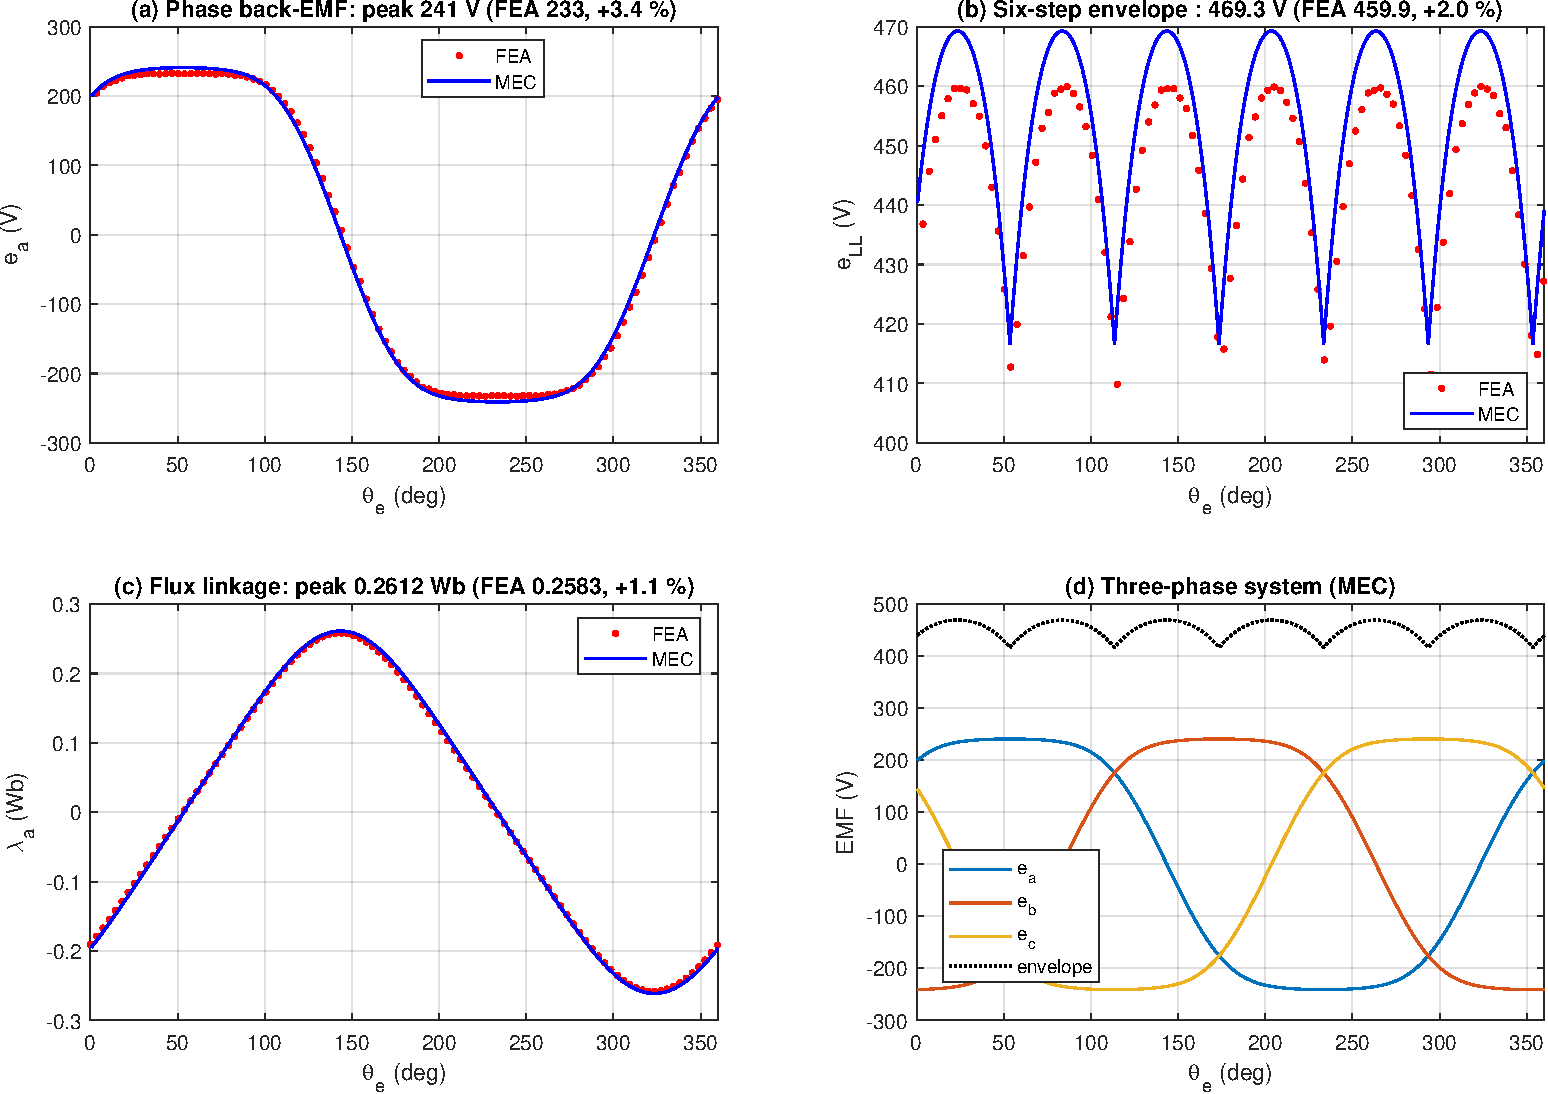
\includegraphics[width=\textwidth,height=0.44\textheight,keepaspectratio]{BLDC_FIG3_bemf.pdf}
\caption{Back-electromotive force and flux linkage at \SI{1500}{\rpm}.
\textbf{(a)} Phase back-electromotive force over one electrical period.
\textbf{(b)} Six-step line-to-line envelope. \textbf{(c)} Flux linkage,
from which the first two follow by differentiation. \textbf{(d)} The
three-phase system computed by the network, shown to establish that the
waveform is balanced and not merely correct on one phase.
A single angular alignment, established on the flux linkage, the
primary, non-differentiated quantity, is used for all three views.}
\label{fig:bemf}
\end{figure*}

\begin{figure*}[!tb]
\centering
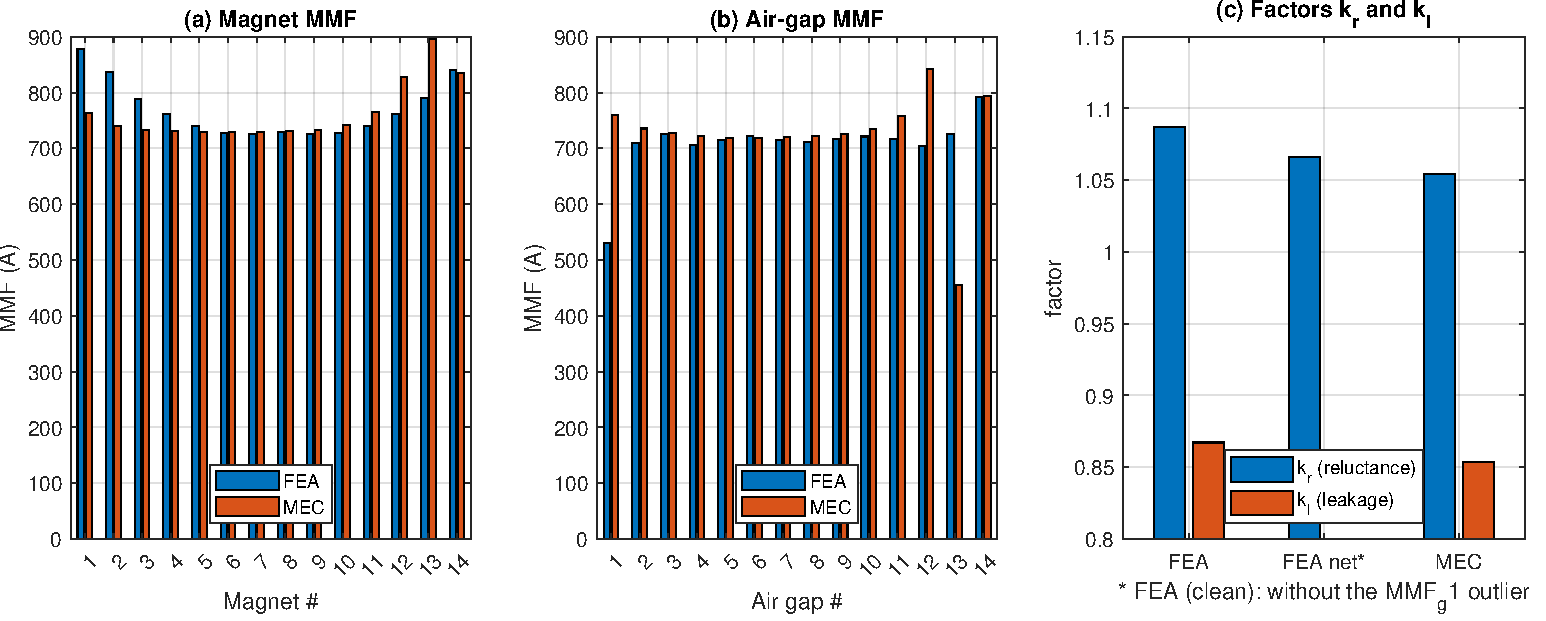
\includegraphics[width=\textwidth,height=0.44\textheight,keepaspectratio]{BLDC_FIG2_circuit.pdf}
\caption{Internal magnetic circuit. \textbf{(a)} Magnetomotive force
across each magnet. \textbf{(b)} Magnetomotive force across each gap.
\textbf{(c)} The reluctance factor $k_{\mathrm{r}}$ and the leakage
factor $k_{\mathrm{l}}$ that the first two define. The quantities are
those from which the reluctance factor
$k_{\mathrm{r}}$ and the leakage factor $k_{\mathrm{l}}$ follow with the
exact definitions read from the reference project. The single gap
magnetomotive force of \SI{531}{\ampere} discussed in
Section~\ref{sub:kr} is visible against its thirteen neighbours.}
\label{fig:circuit}
\end{figure*}

\begin{figure*}[!tb]
\centering
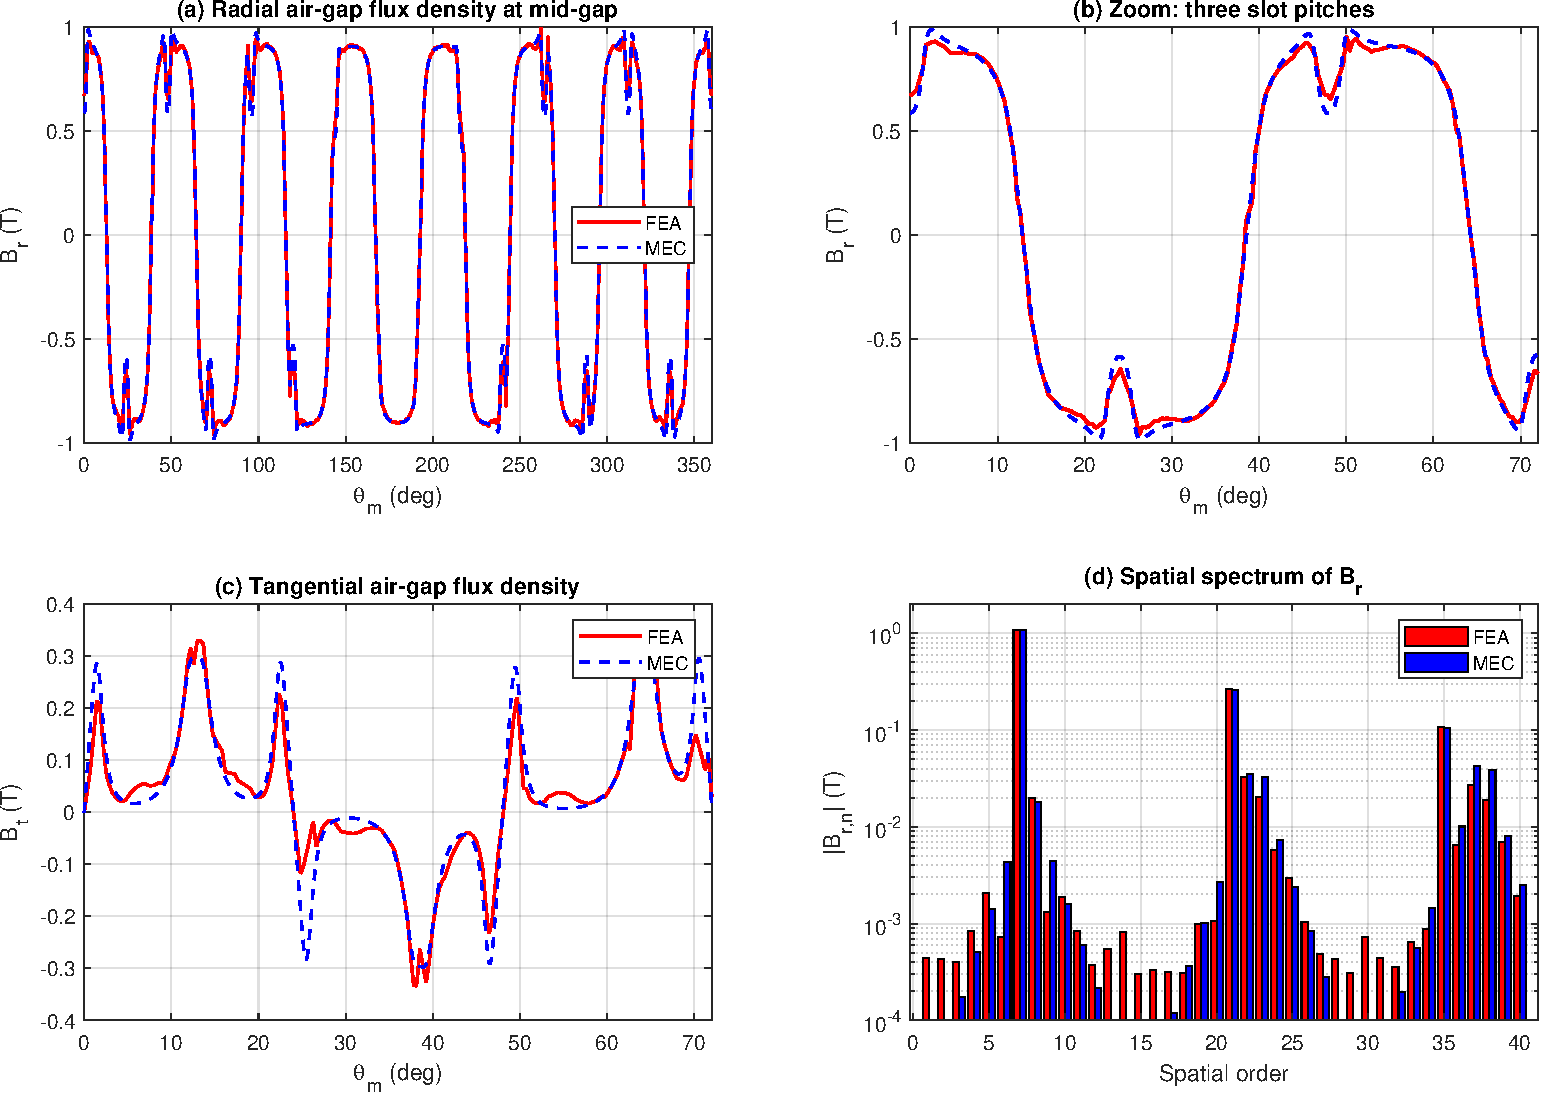
\includegraphics[width=\textwidth,height=0.44\textheight,keepaspectratio]{BLDC_FIG1_champ.pdf}
\caption{Air-gap flux density of the 15/14 PMSM at no load, DtN operator
against two-dimensional finite elements. \textbf{(a)} Radial component
at mid-gap along the whole bore. \textbf{(b)} The same over three slot
pitches, where the slot modulation becomes resolvable. \textbf{(c)}
Tangential component at mid-gap. \textbf{(d)} Spatial spectrum of the
radial component, on which the fundamental and the slot sidebands are
read separately. The tangential component, which a radial-branch network
cannot produce, follows from \eqref{eq:Bt_gap} at no additional cost.}
\label{fig:field}
\end{figure*}

\paragraph{The value of $\mu_{\mathrm{r}}$, and what depends on it.}
The linear solver is used for a stated reason: the reference is an
unsaturated magnetostatic study, and confronting it with a saturated
solution would compare two different functionals. The \emph{value}
\num{3000} deserves its own sentence, because it is not neutral.
Sweeping it over \numlist{2000;3000;5000} on the chain of
Table~\ref{tab:pmsm} moves the tabulated deviations as follows: the
fundamental air-gap flux density from \SI{+0.18}{\percent} to
\SI{+0.41}{\percent}, the mean $\lvert B_r\rvert$ from
\SI{+0.00}{\percent} to \SI{+0.21}{\percent}, the first slot sideband
from \SI{-17.6}{\percent} to \SI{-9.9}{\percent}, and the synchronous
inductance from \SI{-0.64}{\percent} to \SI{+0.71}{\percent}.

\emph{Two of these move by more than the deviation they carry}, and this
must be said rather than left implicit: on $\lvert B_r\rvert$ the spread
is \num{0.21} point against a mean deviation of \num{0.11}, and on
$L_{\mathrm{d}}$ it is \num{1.35} against \num{0.49}. The
\SI{0.10}{\percent} agreement on $L_{\mathrm{d}}$ is therefore a
property of this permeability as much as of the formulation, and the
row is to be read with that reservation. On $B_{g1}$ and on the
sideband, by contrast, the spread is smaller than the deviation and the
conclusions are insensitive to the choice.

\paragraph{One configuration, declared.}
The table is produced by a single execution, in a single configuration,
and this deserves a word because the alternative is common and
misleading. It would be possible to report each row in whichever solver
setting suits it, the linear solution where the reference is an
unsaturated magnetostatic test, the Newton solution where it is a
saturated field, and the resulting table would look better. It would
also no longer describe one model. Every row below is the linear
solution at $\mu_{\mathrm{r}}=\num{3000}$, chosen because the
inductances, $k_{\mathrm{r}}$ and $k_{\mathrm{l}}$ are compared against a
\SI{1}{\ampere} magnetostatic reference in which the iron is not
saturated, and confronting an unsaturated reference with a saturated
solution would compare two different functionals of the field. The price
of that consistency is paid on the rows where saturation does matter,
and it is visible: the field rows should be read alongside
Table~\ref{tab:convb}, which measures what the solver does to a local
quantity on the same meshes.

\paragraph{Integral quantities are markedly improved by the mesh.}
The flux linkage, the back-electromotive force and the six-step envelope
integrate the field over a whole tooth. The mesh model reaches
\SI{+0.24}{\percent} on flux linkage against \SI{+1.11}{\percent} for the
lumped network, \SI{+2.48}{\percent} against \SI{+3.37}{\percent} on the
phase back-electromotive force, and \SI{+1.01}{\percent} against
\SI{+1.91}{\percent} on the six-step envelope. By the amplification
argument of Section~\ref{sub:cost} this is not cosmetic: at the rated
operating point the phase current is a small difference of two large
numbers, and a \SI{1}{\percent} error on the electromotive force is
amplified by a factor of 2.2 on the current.

\paragraph{The inductances obtained without any added formula are the
more accurate.}
The synchronous inductance is within \SI{0.10}{\percent} on the mesh
against \SI{1.24}{\percent} on the fitted lumped model. In the lumped
model, \SI{60}{\percent} of $L_{\mathrm{a}}$ comes from an analytical
slot permeance; in the mesh model it is a solved quantity, and the
self-inductance alone is within \SI{0.34}{\percent} against
\SI{1.12}{\percent}.

That figure carries a reservation which is stated here rather than left
for a reader to find in the table. The synchronous inductance is
$L_{\mathrm{d}}=L_{\mathrm{a}}-M$, and on the mesh the two errors have
opposite signs: $L_{\mathrm{a}}$ is high by \SI{0.34}{\percent} and $M$
is low by \SI{5.48}{\percent}, so they subtract. With the reference
mutual inserted in place of the computed one, the deviation on
$L_{\mathrm{d}}$ would be \SI{0.33}{\percent} instead of
\SI{0.10}{\percent}, a factor of \num{3.2}. The
\SI{0.10}{\percent} is therefore exact and reproducible, but it is not
independent evidence about $L_{\mathrm{a}}$ and $M$ separately, and it
should not be read as such.

\paragraph{The mutual brackets the reference without reaching it, and
the bracket is physical.}
$M$ is low by \SI{5.48}{\percent} on the mesh and high by
\SI{4.09}{\percent} on the lumped network. For an integral quantity this
is unusual enough to warrant an explanation rather than a note. The two
models do not couple the phases by the same path. In the mesh, the
magnetomotive force of phase A is injected into the radial branches of
the coil layers and the flux captured by B and C travels through the
tangential branches and the annulus; part of the coupling flux is free
to leak into the air cells of the slot, and $|M|$ comes out low. The
lumped network has no slot cells: whatever flux leaves tooth A must
reach B or C, and $|M|$ comes out high. The bracket is the signature of
the two topologies, not an accident of either.

\paragraph{One row runs the other way, and it depends on the mesh.}
The pole-to-pole dispersion of the magnet magnetomotive force is
\SI{6.37}{\percent} at one shoe layer, \SI{5.96}{\percent} at two,
\SI{6.81}{\percent} on the lumped network, against \SI{6.59}{\percent} in
the reference. The finer of the two mesh columns is thus the further
away, while the coarser is the closest of all three models. This is the
general behaviour of the table, and it is one-sided. Counting the
seventeen deviations of Table~\ref{tab:pmsm} entry by entry, the coarser
column is the closer on \emph{twelve}, the finer on four, with the
back-electromotive force a tie: the finer column is better only on the
tangential field, on $k_{\mathrm{l}}$, on the magnetomotive force per gap
and on the mutual inductance. Refining the shoe therefore degrades the
majority of the quantities it was refined to improve.

That result is not an anomaly to be reported and left; it is the
signature of the mechanism established in
Section~\ref{sub:corner}. Refinement converges only towards a bounded
limit, and the shoe sub-region is precisely where the field is not
bounded: the tooth-tip re-entrant corner carries an $r^{\lambda-1}$
singularity with $\lambda<1$~\cite{grisvard1985,meixner1972}, so the peak linear flux density rises with
every added layer instead of settling. A shoe discretisation cannot
converge towards a field that does not exist, and the fact that twelve
of seventeen quantities move away under refinement is the integral
evidence of what Section~\ref{sub:corner} demonstrates locally. Both
columns are therefore reported as a bracket, and neither is presented as
\emph{the} refined model, not because the evidence is balanced, which
it is not, but because a refinement that does not converge does not
produce a reference value. The dispersion itself is the slotting seen from the rotor, hence
a local quantity concentrated at the tooth tips, and local quantities
are the ones this formulation reports as bounded
(Section~\ref{sec:bounds}).





\subsection{Reluctance Factor and an Anomaly in the Reference Solution}
\label{sub:kr}

The reluctance factor requires a word, because it is the first
indication of the point developed in Section~\ref{sec:audit}: that the
reference itself carries uncertainty. Of the fourteen gap magnetomotive
forces from which $k_{\mathrm{r}}$ is built, thirteen lie between
\SI{704}{\ampere} and \SI{792}{\ampere} and one returns
\SI{531}{\ampere} (Fig.~\ref{fig:circuit}). That magnet is adjacent to
the one reporting \SI{792}{\ampere}, and no physical mechanism produces
a \SI{33}{\percent} step between neighbouring poles in a machine whose
magnet-to-magnet dispersion, measured on the same solution, is
\SI{6.6}{\percent}.

Retaining the outlier gives the value published by the reference
project, $1.0869$, and a mesh deviation of \SI{-1.9}{\percent};
excluding it gives $1.0664$ and \SI{+0.03}{\percent}. Both are reported
in Table~\ref{tab:pmsm} and neither is selected, because selecting would
convert a property of the reference into a property of the model. Two
observations bear on which is the more likely: the anomaly appears on a
quantity sampled along a single radial line per pole, and
$k_{\mathrm{l}}$, which is built from the same field solution but
integrates over the whole magnet surface, shows no such step.

\subsection{Complete Air-Gap Flux-Density Spectrum}
\label{sub:spectrum}

Table~\ref{tab:spectrum} lists every spatial order the model computes,
rather than the subset that supports the argument. The working harmonics
$3p$ and $5p$ agree within \SI{2.4}{\percent}, and the fundamental
within \SI{0.3}{\percent}. The first slot sidebands
$\nu=|N_{\mathrm{s}}-p|=8$ and $\nu=N_{\mathrm{s}}+p=22$ agree within
\SI{8}{\percent}.

The second slot sidebands do not. At $\nu=|2N_{\mathrm{s}}-p|=23$ and
$\nu=2N_{\mathrm{s}}+p=37$ the model overshoots the reference by
\SI{61}{\percent} and \SI{58}{\percent}. These are the largest field
errors in this work and they are reported because omitting them would
misrepresent what the formulation delivers.

Their origin is the one already identified for the first sidebands. Both
families are produced by the same modulation of the air-gap permeance
under the slot opening, and that modulation is governed by the field at
the tooth-tip corner, which is singular (Section~\ref{sec:bounds}). The
second sidebands sample the corner region more sharply than the
first, their angular wavelength is roughly half the slot opening, so
the same unresolved singularity produces a larger relative error. The
direction is consistent: the network overshoots at $\nu=22$, 23 and 37,
and the overshoot grows with order. Orders beyond the first sidebands
should therefore be read as an indicator of corner resolution, not as
validated outputs.

\begin{table*}[!t]
\centering
\footnotesize
\begin{tabular}{llrrr}
\toprule
Order & identification & Network & FEA & deviation \\
\midrule
$p=7$  & fundamental                      & 1.0776 & 1.0746 & $+0.3\%$ \\
8      & $|N_{\mathrm{s}}-p|$             & 0.0181 & 0.0197 & $-8.1\%$ \\
21     & $3p$                             & 0.2593 & 0.2657 & $-2.4\%$ \\
22     & $N_{\mathrm{s}}+p$               & 0.0352 & 0.0328 & $+7.6\%$ \\
23     & $|2N_{\mathrm{s}}-p|$            & 0.0326 & 0.0202 & $+61.1\%$ \\
35     & $5p$                             & 0.1047 & 0.1067 & $-1.9\%$ \\
37     & $2N_{\mathrm{s}}+p$              & 0.0427 & 0.0271 & $+57.6\%$ \\
\bottomrule
\end{tabular}
\caption{PMSM air-gap flux density at no load: complete spatial spectrum
computed by the model. Lumped network, mid-gap radius, flux density in
tesla. Orders 23 and 37 are the second slot sidebands and are governed
by the tooth-tip singularity of Section~\ref{sec:bounds}.}
\label{tab:spectrum}
\end{table*}

\subsection{Magnet Eddy-Current Losses}
\label{sub:pmloss}

The magnet losses follow from \eqref{eq:Br_mag} without additional
hypothesis. Writing the vector potential in the rotor frame and imposing
zero net current over the \emph{whole} cross-section of each magnet,
\begin{equation}
\begin{aligned}
J_z &= -\sigma\,\widetilde{A},
\qquad
P = \sigma L \int_S \widetilde{A}^{\,2}\,\mathrm{d}S ,\\[1ex]
\widetilde{A} &\equiv \frac{\partial A}{\partial t}
- \Bigl\langle \frac{\partial A}{\partial t}\Bigr\rangle_{S},
\end{aligned}
\label{eq:pmloss}
\end{equation}
where $\sigma$ is the magnet conductivity and $S$ the magnet section.

\emph{The validity condition should be stated with the formula.}
Equation~\eqref{eq:pmloss} imposes a zero net current without letting the
induced currents react on the field, which is licit only when the skin
depth greatly exceeds the magnet thickness. At the dominant slotting
frequency seen from the rotor, $f=N_{\mathrm{s}}n/60=\SI{422}{\hertz}$
at the no-load test speed, with $\sigma=\SI{555556}{\siemens\per\metre}$
and $\mu_{\mathrm{r}}=\num{1.0390}$, the skin depth is
$\delta=\SI{32.25}{\milli\metre}$ against a magnet thickness of
\SI{3.5}{\milli\metre}, a ratio of \num{9.2}. The reaction field is
therefore neglected, and the assumption would fail on a thicker or more
conductive magnet, or at substantially higher speed. This is a condition
of validity and not a validation: the loss remains between
\SI{25}{\percent} and \SI{39}{\percent} below the reference whichever
way it is read.

Two implementation points are decisive and are reported because both are
easy to get wrong and neither is visible in the result. The zero-current
constraint must be imposed over the entire magnet section: applying it
ring by ring removes the radial variation of $\partial A/\partial t$
, strong here, since the slotting field decays as
$\cosh(n\ln(r/\rmi))$ through the magnet, which is precisely the
$A_n$--$C_n$ structure of \eqref{eq:Br_mag}, and underestimates the
loss by a factor of two to four. And the time derivative must be taken
on the coefficients \emph{already expressed in the rotor frame}:
differentiating the stator-frame coefficients and adding a rotation term
$n\omega$ separately subtracts two nearly equal quantities, the
synchronous component being some 400 times larger than the slotting
modulation that survives in the rotor frame, and inflates the result by
two orders of magnitude.

\paragraph{What the chain returns, and against what.}
Table~\ref{tab:pmloss} reports the losses at no load from a single
frozen chain, at a truncation whose convergence is established rather
than assumed: the computed loss moves by \SI{0.2}{\percent} between
$N_p=181$ and $N_p=481$ rotor positions, a factor of \num{2.7} in
sampling. The two rows differ only in where the field seen by the magnet
comes from, the one-branch-per-tooth network, or the polar mesh, and
that difference is the result of this subsection.

\begin{table}[!ht]
\centering
\begin{threeparttable}
\footnotesize
\begin{tabular}{lrrr}
\toprule
Source of the field & $P$ (W) & FEA (W) & deviation\\
\midrule
one-branch-per-tooth network & 0.2036 & 0.334 & $-39.1\%$\\
polar mesh                   & 0.2516 & 0.334 & $-24.7\%$\\
\bottomrule
\end{tabular}
\begin{tablenotes}[flushleft]\footnotesize
\item Chain frozen for this quantity: $N_p=241$, \SI{1688}{\rpm},
$\sigma=\SI{5.5556e5}{\siemens\per\metre}$, $k_{\mathrm{f}}=\num{0.325}$.
\end{tablenotes}
\end{threeparttable}
\caption{Magnet eddy-current losses at no load. The two rows differ only
in the source of the field seen by the magnet.}
\label{tab:pmloss}
\end{table}

\paragraph{The result is that the field source matters, by fourteen
points.}
Refining the source of the field from a single tooth branch to the polar
mesh moves the loss from \SI{-39.1}{\percent} to \SI{-24.7}{\percent} of
the reference. That is the measurable contribution of the mesh to this
quantity, and it is the publishable result of this subsection.

What is \emph{not} claimed is that the chain is validated at no load. An
earlier version of this work reported \SI{0.342}{\watt} here, and hence
an agreement within \SI{2.4}{\percent}. That value came from a second
routine, the on-load loss integrator called at zero current, which
returned \SI{0.3416}{\watt} on the same operating point and against the
same reference, a factor \num{1.68} above the frozen chain. \emph{The
second routine was wrong, and the cause is a single sign.} Its
transformation to the rotor frame carried the wrong sign on the
sine-projected part of the surface potential, which makes the
\emph{synchronous} component, by far the largest, and the one the
magnet sees as static, turn at $2p\omega$ in the frame where the time
derivative is taken. Its derivative then entered the loss.

The diagnosis does not compare one implementation against the other,
which would settle nothing, nor against the finite-element reference,
against which constants have been fitted. It uses a case whose answer is
known before the computation. Impose a bore potential that rotates
exactly with the rotor,
$u_{\mathrm{s}}(\theta_{\mathrm{s}},\varphi)=\cos p(\theta_{\mathrm{s}}
-\varphi)$: in the magnet frame that field is static, the induced
current density is identically zero, and so is the loss. The frozen
chain returns \SI{9.5e-32}{\watt}. The second routine returned
\SI{3.4e-5}{\watt}---\num{3.56} times the entire scale of the problem.
A companion case, a harmonic fixed to the stator for which
$\mathrm{d}A/\mathrm{d}t$ is written in closed form and passed through
the same quadrature and the same zero-net-current constraint, is
reproduced by both routines to \SI{0.09}{\percent}. The two cases
together localise the defect in the frame transformation and nowhere
else: the quadrature and the derivative were sound in both.

Corrected, the second routine returns \SI{0.2120}{\watt} on the same
point, \SI{-36.4}{\percent} of the reference, and the ratio between the
two routines falls from \num{1.68} to \num{1.04}. The
\SI{2.4}{\percent} agreement was an artefact. The consequence is not
confined to one number: it removes the dichotomy the earlier version
relied on, a no-load point said to validate the whole formulation,
against an on-load point left open, and Section~\ref{sub:pmloss_bound}
states what replaces it. The magnet loss is a single deviation of the
same order at both operating points, not two qualitatively different
situations. The on-load figure of Table~\ref{tab:load} moves by
\SI{1}{\percent} only, and that asymmetry is itself a check: on load the
loss is dominated by the six-step armature field, which does not turn
with the rotor and which the faulty sign therefore left alone.

The magnitude is consistent with the position this paper takes on local
quantities. The loss integrand is $\widetilde{A}^{\,2}$, so it weights
the slotting modulation, the part of the field carried by the sidebands
of Section~\ref{sub:spectrum}, which the tooth-tip singularity governs
and which neither model resolves. A quantity built from the square of an
unconverged component inherits its status, and the ordering of the two
rows is the evidence: the model that resolves the tooth tip better is
the one that is closer.

One point of resolution closes the subsection. What remains of the
\num{1.04} between the two routines is quadrature, and it can be measured
rather than argued. The frozen chain integrates the magnet thickness on
seven equally spaced radii, while the tooth field varies as
$\cosh(n\ln(r/\rmi))/\sinh(n\Um)$ and is therefore concentrated against
the gap surface, which seven equal steps do not resolve. Held at a common
field source, at eighty-one radii clustered towards $\Rro$ and
\num{1440} angular steps, the two routines return the same
\SI{0.210449}{\watt} and agree to
\SI[retain-negative-zero]{-0.00}{\percent}, the sign of a difference below
the printed resolution. \emph{They are
one formulation evaluated at two resolutions, not two models}, which is
what removes the choice between them instead of settling it. The
converged figure is quoted as a measure of the radial quadrature and not
as a replacement: Table~\ref{tab:pmloss} keeps the chain frozen at the
settings under which every other quantity of this section was computed,
and the \SI{-39.1}{\percent} it carries is unchanged.

\subsection{System-Level Drive Model}
\label{sub:drive}

\subsubsection{Saturable Flux-Linkage and Torque Maps}
\label{sub:map}

At start-up the inverter applies the full dc bus across two phases in
series and the current reaches \SI{23}{\ampere}, so that the coil
magnetomotive force is \SI{3500}{\ampere} (ampere-turns) and the armature flux is
4.7 times the magnet flux. In that regime neither the magnet flux
linkage nor the inductance is a constant. The same network, solved with
the real $B(H)$ characteristic over a grid in rotor position and in the
current plane, supplies
\begin{equation}
\lambda_k\!\left(\theta,i_\alpha,i_\beta\right),
\qquad
T\!\left(\theta,i_\alpha,i_\beta\right),
\label{eq:map}
\end{equation}
the torque being obtained from \eqref{eq:torque}, the only form that
remains valid when $\lambda$ is no longer linear in $i$. Between
\SI{0}{\ampere} and \SI{25}{\ampere} the map shows the line inductance
collapsing from \SI{104.3}{\milli\henry} to \SI{12.1}{\milli\henry}, and
the \emph{incremental} flux-linkage gradient
$\partial\psi_{ab}/\partial\theta$ falling from
\SI{3.01}{\weber\per\radian} to \SI{0.68}{\weber\per\radian}. The second
figure is an incremental quantity at the operating point and not a
collapse of the magnet flux itself, which the armature cannot suppress:
it measures the local flattening of $\psi_{ab}(\theta)$ once the teeth
are driven deep into saturation.

A modelling point deserves emphasis, and a claim made in an earlier
version of this work has to be withdrawn with it. The classical slot
permeance $\lambda=h/3b$ assumes infinitely permeable iron on both sides
of the slot and accounts for \SI{60}{\percent} of the line inductance;
leaving it unsaturable forbids the inductance to fall below
\SI{64}{\milli\henry} at any current. The leakage flux itself crosses
the teeth, at \SI{10}{\ampere} it adds some \SI{0.9}{\tesla} there, so
the air permeance is placed in series with the reluctance of the iron
that closes its path, evaluated with the permeability already computed
by the nonlinear network. That correction was said to restore the
physical collapse. Regeneration does not support the claim. The
saturable slot leakage falls only to $\lambda_{\mathrm{ef}}/\lambda_{\mathrm{tot}}
=\num{0.991}$ at \SI{5}{\ampere} and \num{0.810} at \SI{23}{\ampere},
which is too little to carry the curve. The published characteristic
falls by a factor \num{11.0} between \SI{0}{\ampere} and
\SI{25}{\ampere}; the raw output of the same network falls by
\num{3.4}, and the network without its tangential bridge by \num{1.8}.
The published factor is obtained by subtracting a constant
\SI{29.4}{\milli\henry}, calibrated at zero current, from a quantity
that itself descends only to \SI{38.9}{\milli\henry}.

The premise of that subtraction is that the excess is a path in air and
therefore does not saturate, so the correction may be taken as a
constant. It is not: the difference between the network with and without
the tangential bridge is $+\SI{29.9}{\milli\henry}$ at zero current and
$-\SI{19.3}{\milli\henry}$ at \SI{25}{\ampere}, changing sign over a
range of \SI{49.2}{\milli\henry}. The subtraction is exact where it was
calibrated and increasingly wrong away from it, and this also accounts
for the loss of grid convergence at high current: at \SI{25}{\ampere}
the published value is the difference of two numbers of comparable size,
so any relative error on the raw quantity is amplified by \num{4.1}
there, against \SI{0.3}{\percent} dispersion at \SI{5}{\ampere}.

Two reservations bound what may be concluded from the comparison with
the reference, and they run in the direction of caution rather than
of exoneration. The reference contradicts itself at zero current:
its magnetostatic study gives \SI{104.68}{\milli\henry} with the magnets
removed and its transient \SI{72.25}{\milli\henry} with them present, a
gap of \SI{31}{\percent} at an excitation where no armature saturation
is possible, and the network agrees with the magnetostatic value to
\SI{0.35}{\percent}. And the transient is screened by induced currents,
the solid loss reaching \SI{52.3}{\percent} of the Joule loss at the
first sample, the relative weight being largest precisely at the low
currents where the measurement is wanted. The deviations quoted against
the transient are therefore an \emph{upper bound} on the quasi-static
error of the model instead of a measurement of it; separating the two
would require a magnetostatic current sweep at fixed rotor position,
which is left to further work.

One further caution attaches to how this quantity is displayed. The
characteristic is an average over rotor position, and the underlying
quantity is not weakly dependent on that position: at
\SI{10}{\ampere} it ranges from \SI{31.6}{\milli\henry} to
\SI{105.9}{\milli\henry} over one revolution, a factor above three,
against an average of \SI{63.6}{\milli\henry}. The drive model does not
use the average, it interpolates the phase inductances at the
instantaneous position, so the plotted curve is a summary of the map
and not the quantity the simulation integrates. It should be read as
such.

\subsubsection{Inverter and Mechanical Subsystem Models}

The converter is transcribed from the finite-element circuit: split
$\pm V_{\mathrm{dc}}/2$ supply, three half-bridges, position-triggered
\ang{120} conduction, freewheeling diodes and an isolated star point.
The commutation law was verified against the gate probes of the
reference run, measured period \ang{51.44} mechanical against
$720/N_{\mathrm{m}}=\ang{51.4286}$, and firing angles within
\ang{1.6} of the netlist values.

\subsubsection{On-Load Transient Response and Speed Sweep}
\label{sub:drive_results}

Figs.~\ref{fig:load_sat}, \ref{fig:load} and~\ref{fig:load_conv} show
the on-load transient computed entirely by the network drive model, and
Table~\ref{tab:load} reports its steady state. Their panels are as
follows. Fig.~\ref{fig:load} follows the electrical and mechanical
start-up: panel~(a) the speed against the reference, panel~(b) the phase
current through the transient, panel~(c) the same current in the settled
regime against electrical angle, and panel~(d) the dc-bus current, which
is the quantity the supply sees. Fig.~\ref{fig:load_conv} follows the
conversion at the same operating point: panel~(a) the electromagnetic
torque, panel~(b) the Joule loss, panel~(c) the efficiency, and
panel~(d) the loss breakdown by mechanism, which is what makes the
efficiency figure interpretable rather than merely reported.

Fig.~\ref{fig:sweep} and Table~\ref{tab:sweep} report the sweep at
constant dc-bus voltage. Its six panels are read in pairs: panels~(a)
and~(b) give torque and power against speed, panels~(c) and~(d) the
current and the voltage envelope that bound them, and panels~(e)
and~(f) the efficiency and the loss distribution along the sweep. The
envelope of panel~(d) is the quantity that limits the others, and it is
the reason the deviations of this figure are discussed together rather
than one by one; Fig.~\ref{fig:score} synthesises the deviation
from the reference over the twenty-nine quantities computed, of which
twenty-one fall within \SI{5}{\percent}. Three of the twenty-nine are
declared in this paper as not validated---the two magnet-loss entries,
whose reference cannot resolve the quantity being compared, and the
standstill torque, excluded from the comparison in
Section~\ref{sec:methods}. Excluding them, the count is twenty of
twenty-six. It is the second count that should be read, and what the
exclusion buys is the measure of how little the synthesis rests on it:
setting aside three quantities recovers a single entry.

\begin{figure*}[!tb]
\centering
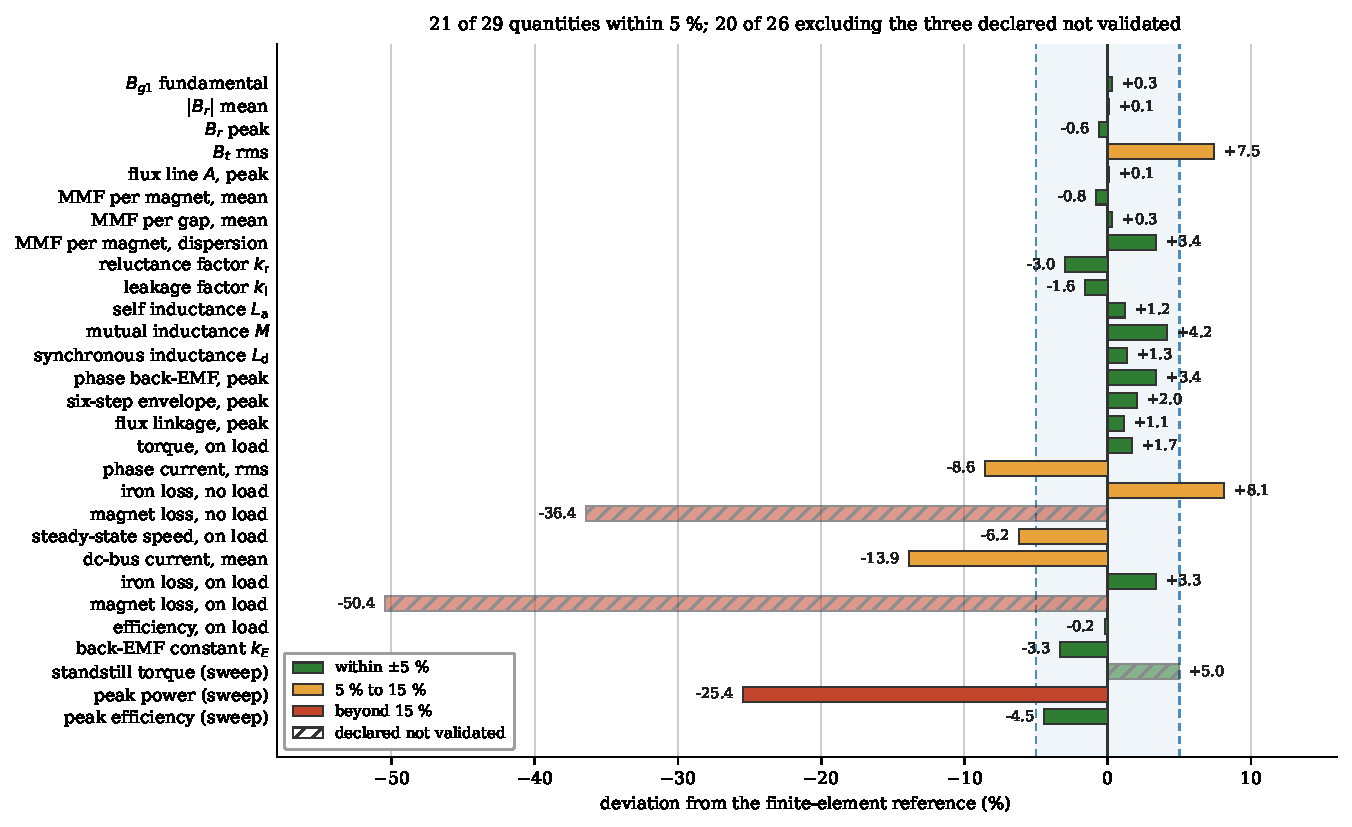
\includegraphics[width=\textwidth,height=0.44\textheight,keepaspectratio]{BLDC_FIG7_scorecard.pdf}
\caption{Synthesis of the PMSM validation, computed throughout on the
\emph{lumped} iron model, the fixed iron representation of the closure
axis of Fig.~\ref{fig:protocol}, and the one every result of this
section uses except the two mesh columns of Table~\ref{tab:pmsm}.
Deviation from the
finite-element reference for the twenty-nine quantities computed by the
program, from the air-gap field to the speed sweep. Twenty-one fall
within \SI{5}{\percent}; excluding the three entries declared in this
paper as not validated, the two magnet-loss bars and the standstill
torque, hatched, the count is twenty of twenty-six. Each bar carries its
own deviation, so both counts can be checked from the figure; the same
twenty-nine values are tabulated in Appendix~\ref{app:scorecard}. The
two efficiency rows are compared as a difference in points, per the rule
of Section~\ref{sub:stats}, and the threshold is applied to that
difference; the counts are unchanged by the convention. Two
quantities lie within one point of the threshold and both lie
inside it, the standstill torque at $+\SI{4.95}{\percent}$.}
\label{fig:score}
\end{figure*}

\begin{figure*}[!tb]
\centering
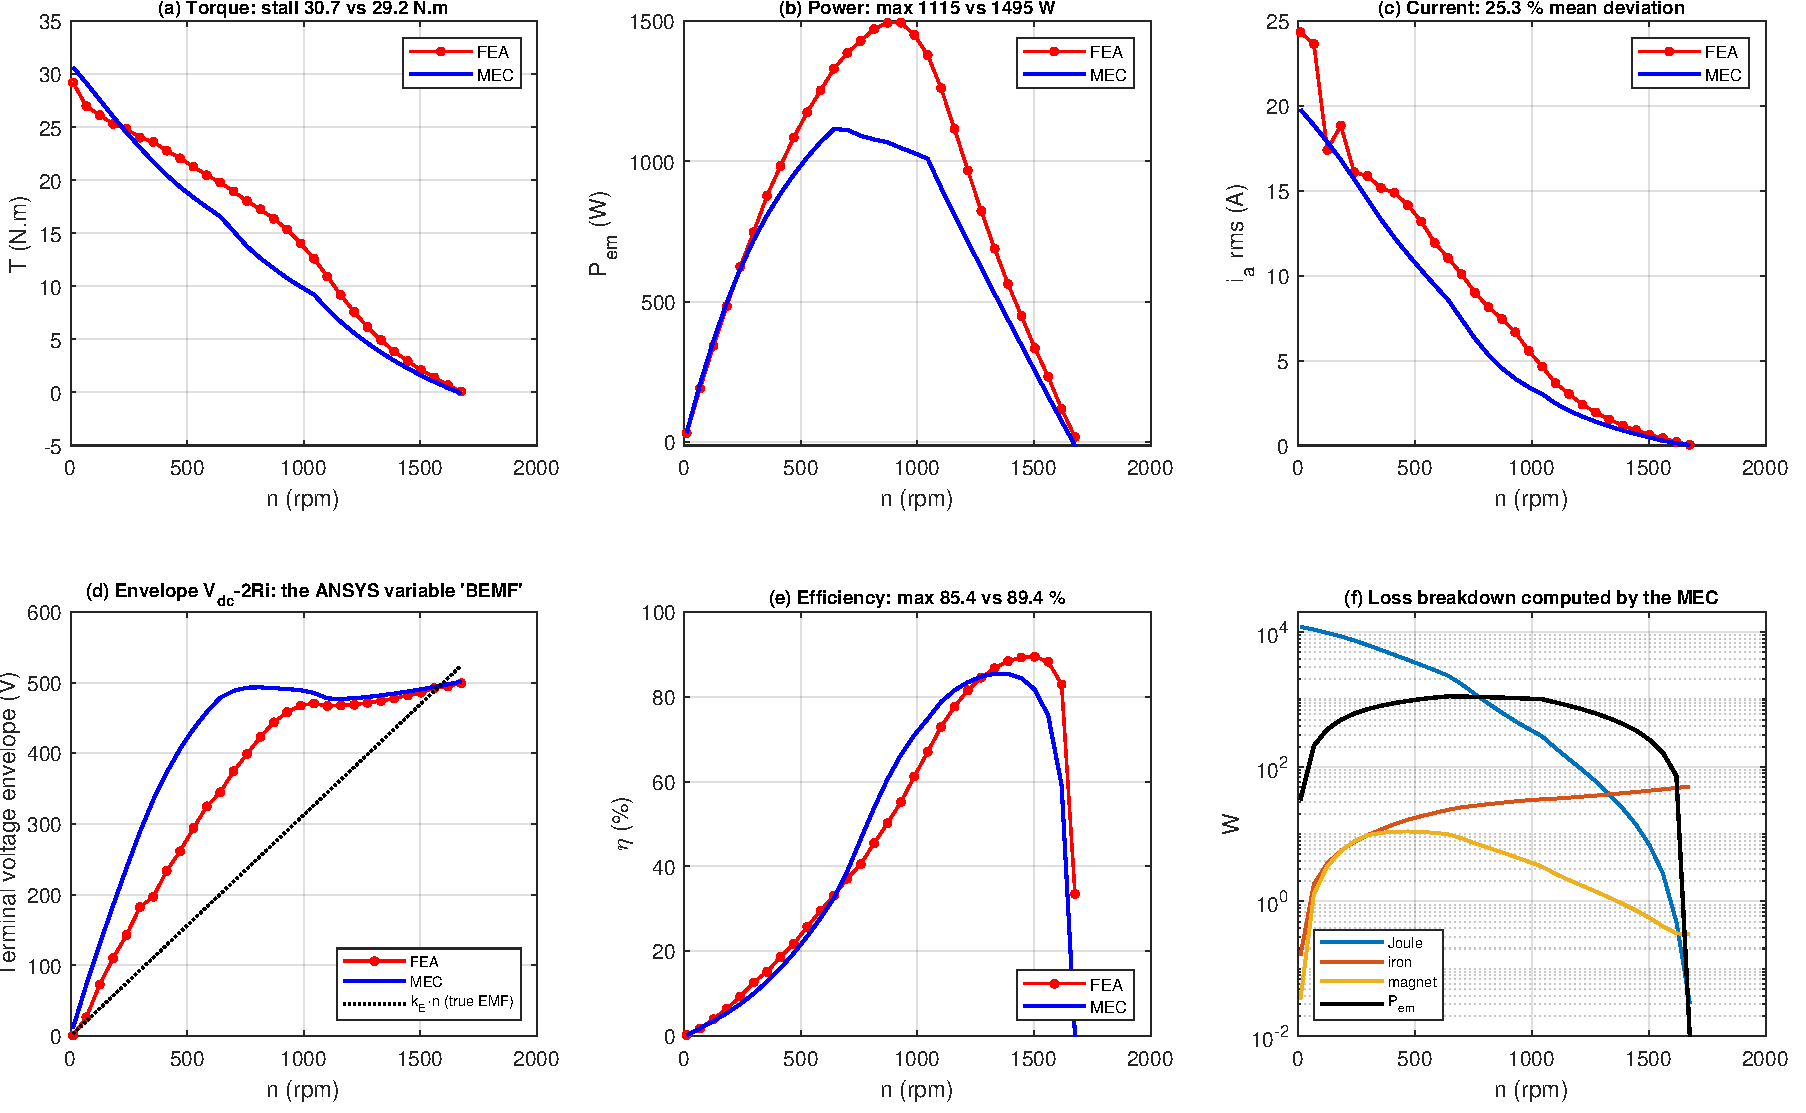
\includegraphics[width=\textwidth,height=0.44\textheight,keepaspectratio]{BLDC_FIG6_balayage.pdf}
\caption{Speed sweep at constant dc-bus voltage. \textbf{(a)} Torque
against speed. \textbf{(b)} Power. \textbf{(c)} Current. \textbf{(d)}
Terminal-voltage envelope, which is the quantity that limits the
others. \textbf{(e)} Efficiency. \textbf{(f)} Loss breakdown computed by
the network along the sweep. The
finite-element variable named \emph{BEMF} is the terminal envelope
$V_{\mathrm{dc}}-2Ri$, not the electromotive force; it is compared as
such, with $k_E n$ shown separately.}
\label{fig:sweep}
\end{figure*}

\begin{table}[!ht]
\centering
\footnotesize
\begin{threeparttable}
\begin{tabular}{lrrr}
\toprule
Quantity & MEC & FEA & deviation \\
\midrule
speed (rpm)                   & 1257  & 1340  & $-6.2\%$ \\
shaft power (W)\tnote{a}      & 651.5 & 682.8 & $-4.6\%$ \\
electromagnetic torque (N\,m) & 4.949 & 4.867 & $+1.7\%$ \\
copper loss (W)               & 69.43 & 71.56 & $-3.0\%$ \\
phase current, rms (A)\tnote{b}& 1.419 & 1.552 & $-8.6\%$ \\
\quad from the copper loss\tnote{b} & 1.505 & 1.528 & $-1.5\%$ \\
iron loss (W)                 & 19.08 & 18.47 & $+3.3\%$ \\
magnet loss (W)\tnote{c}      & 1.578 & 3.183 & $-50.4\%$ \\
efficiency (\%)\tnote{a}      & 86.33 & 86.51 & $-0.2$ p.p. \\
\bottomrule
\end{tabular}
\begin{tablenotes}[flushleft]\footnotesize
\item[a] The two columns are evaluated at different speeds, hence at
different shaft powers; see Section~\ref{sub:drive_results}. Efficiency
follows \eqref{eq:eta} in both columns.
\item[c] This row moved from \SI{1.593}{\watt} when a sign error was
corrected in the rotor-frame transformation of the loss integrator; see
Section~\ref{sub:pmloss}. The on-load figure is almost unaffected
because the dominant term here is the armature field, which does not
turn with the rotor: the network decomposition is
\SI{0.114}{\watt} of slotting against \SI{1.463}{\watt} of six-step
armature.
\item[b] Two values are given because they are not the same measurement,
and the difference between them is informative.
The first is the direct root-mean-square of the computed phase current
over the steady-state window; that window spans 1.256 electrical periods
at \SI{1257}{\rpm}, so the three phases are sampled at different points
of their cycles and the estimate is biased low. The second inverts the
model's own copper loss, $P_{\mathrm{cu}}=3R_{\mathrm{ph}}I^2$ with
$R_{\mathrm{ph}}=\SI{10.2223}{\ohm}$, which is unbiased because
$\sum_k i_k^2$ is very nearly constant under \ang{120} conduction; it is
therefore not an independent check of the copper-loss row. The reference
column of that row is the current the \emph{reference's} own copper loss
implies, formed the same way, so the two are like for like; comparing it
instead against the reference's direct root-mean-square gives
\SI{-3.0}{\percent} and compares two different measurements. Note that
\SI{10.2223}{\ohm} is the network's resistance and
\SI{10.220}{\ohm}, in Table~\ref{tab:machines}, is the one measured on
the reference project, they differ by \SI{0.023}{\percent} and the
table reports each where it belongs. An
integer-period window removes the discrepancy and is the recommended
practice. Separately, the reference's own current and copper loss imply
$R_{\mathrm{ph}}=\SI{9.903}{\ohm}$, \SI{3.2}{\percent} below the value
used by the network: the two models do not share the same winding
temperature. This is unrelated to the air-gap formulation but it bounds
what the copper-loss row establishes, and it is the concrete reason the
measurement protocol of Section~\ref{sub:posture} asks for the
phase resistance four-wire at a \emph{recorded} temperature: a
\SI{3.2}{\percent} discrepancy on a quantity neither model measures is
larger than several of the deviations this paper reports.
\end{tablenotes}
\end{threeparttable}
\caption{PMSM on-load transient, steady state.}
\label{tab:load}
\end{table}

\begin{figure*}[!tb]
\centering
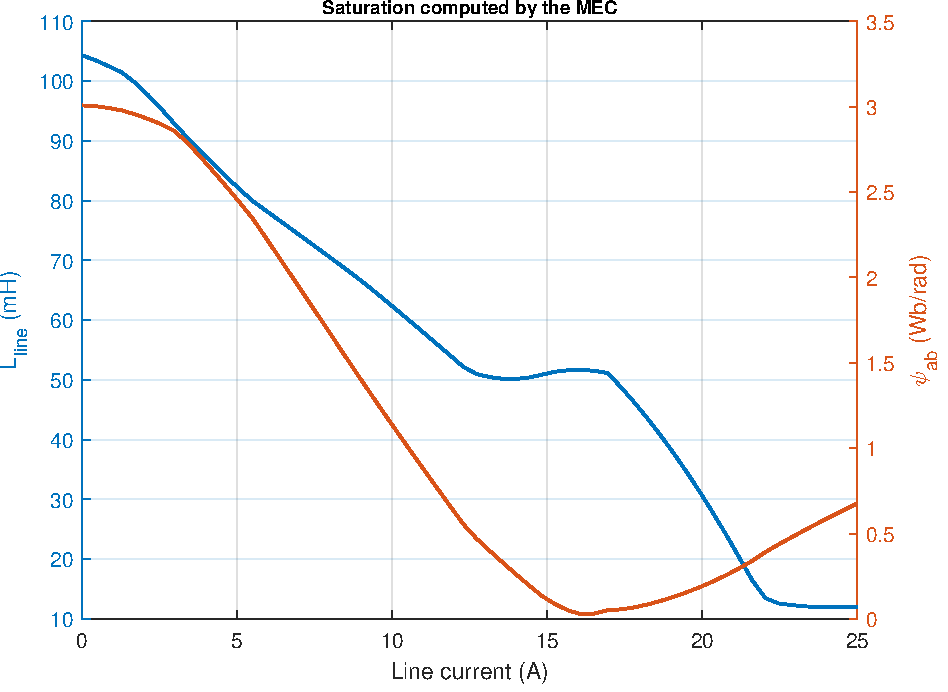
\includegraphics[width=\textwidth,height=0.44\textheight,keepaspectratio]{BLDC_FIG5_3_saturation.pdf}
\caption{Saturation curves $L_{\ell\ell}(i)$ and $\psi_{ab}(i)$ from the
map \eqref{eq:map}. The line inductance falls from
\SI{104.3}{\milli\henry} to \SI{12.1}{\milli\henry} between
\SI{0}{\ampere} and \SI{25}{\ampere}.}
\label{fig:load_sat}
\end{figure*}

\begin{figure*}[!tb]
\centering
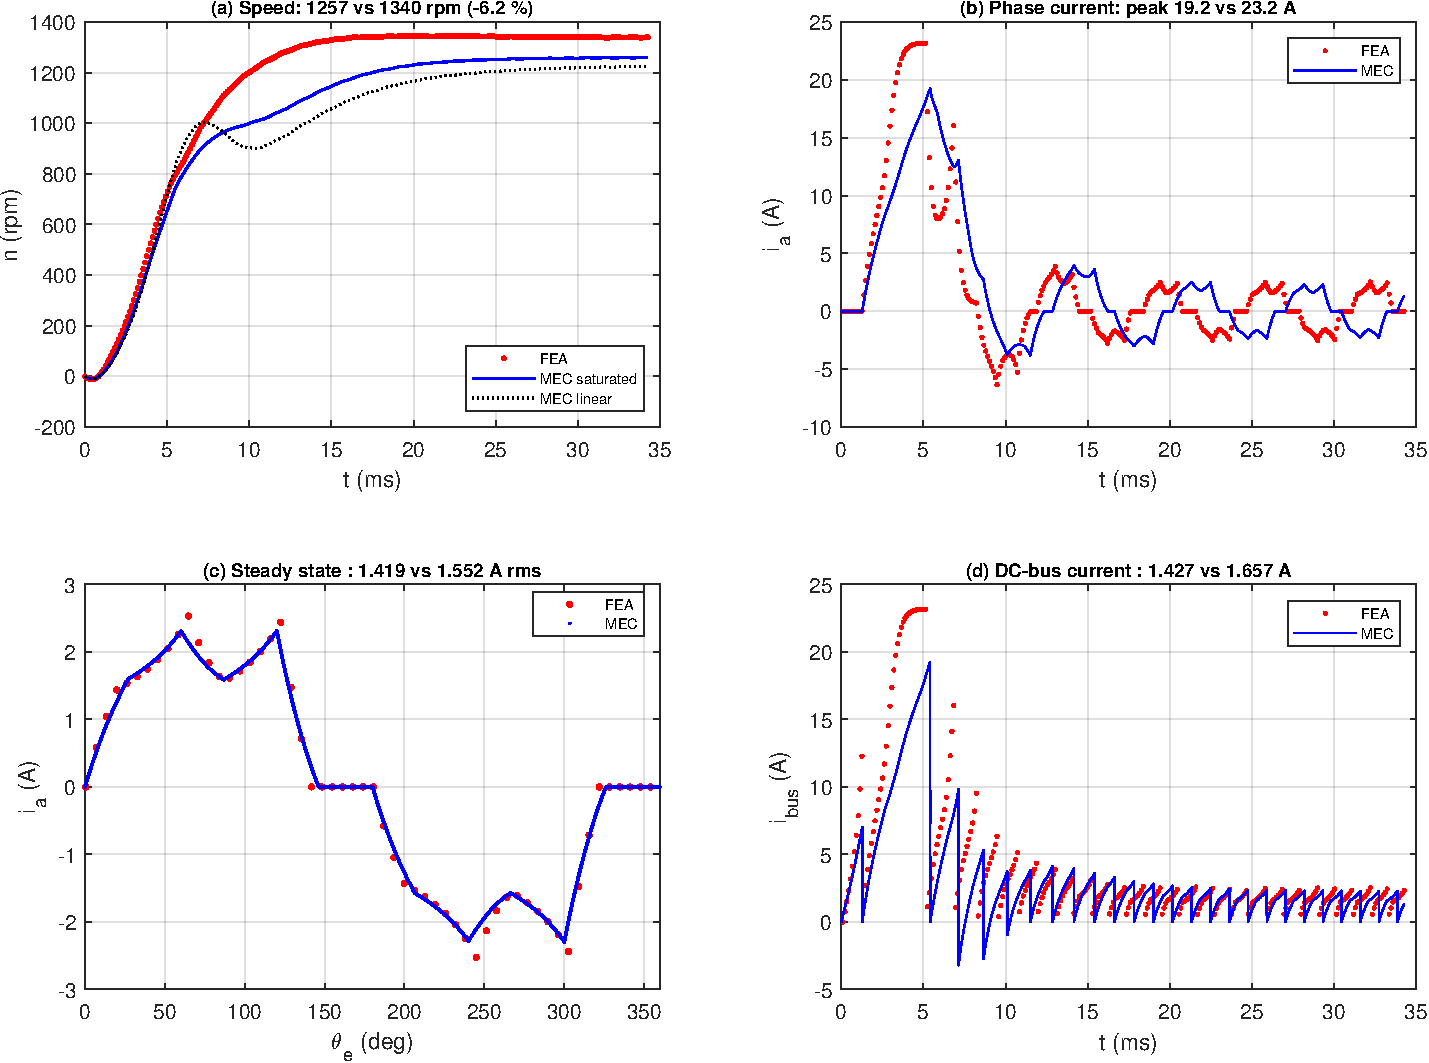
\includegraphics[width=\textwidth,height=0.44\textheight,keepaspectratio]{BLDC_FIG5_1_transient.pdf}
\caption{On-load transient computed entirely by the MEC drive model,
against the finite-element reference. \textbf{(a)} Speed.
\textbf{(b)} Phase current through the transient. \textbf{(c)} The same
current in the settled regime, against electrical angle.
\textbf{(d)} Dc-bus current, the quantity the supply sees.}
\label{fig:load}
\end{figure*}

Three results must be read together, and the reading is not uniformly
favourable.

\emph{The efficiency agrees, but not at the same operating point.} The
efficiency computed with \eqref{eq:eta} differs by \SI{0.2}{\pp}. That
agreement is real but it is obtained at a steady-state speed low by
\SI{6.2}{\percent}, hence at a shaft power of \SI{651}{\watt} against
\SI{683}{\watt}, a difference of \SI{4.6}{\percent}. The two
efficiencies are therefore evaluated at two different points of the
same characteristic, and the figure should be read as ``the loss
structure is reproduced'' rather than as ``the operating point is
reproduced''. It is not.

\emph{The characteristic sags between its end points.} The no-load speed
is reproduced within \SI{1.3}{\percent}. The stall torque agrees within
\SI{5.0}{\percent}, but that agreement cannot be claimed as a
validation: the stall point is the \SI{10}{\rpm} run, which Test~5 of
Section~\ref{sec:audit} shows is not a periodic steady-state average in
the reference. It is quoted for completeness and excluded from the
comparison. Between
them the model runs low, by \SI{25.4}{\percent} on peak power, and the
mean deviation over the twenty-eight points above \SI{100}{\rpm} is
\SI{25.8}{\percent} on torque and power. The cause is the
voltage-limit amplification of Section~\ref{sub:cost} compounded by a
dynamic effect: at mid speed the electrical time constant
$L/2R=\SI{5.19}{\milli\second}$ is comparable to the
\SI{9.83}{\milli\second} electrical period, so the current cannot settle
within a \ang{60} conduction window and both models remain below the
quasi-static value, the network more so. Table~\ref{tab:settle}
quantifies this and shows that it is a property of the drive rather than
of the closure: at \SI{872}{\rpm} the quasi-static current is
\SI{11.12}{\ampere}, the reference reaches \SI{9.14}{\ampere} and the
network \SI{5.59}{\ampere}, both short of the settled value, in the
same direction. A time constant common to both models cannot, however,
account for the network falling twice as far short, so the natural
suspicion is that the saturation map over-saturates at intermediate
current and lengthens the electrical transient artificially. That
hypothesis was tested and does not hold. Comparing the incremental
inductance of the map against the reference at
\SI{2}{}, \SI{5}{} and \SI{10}{\ampere}, the range over which the reference admits an
incremental reading at all, the rotor being effectively fixed only below
\SI{12.27}{\ampere}, and no point beyond it being extrapolated, the map
runs \emph{high}, not low, so refining the current grid moves the
settled current from \SI{5.59}{\ampere} to \SI{5.52}{\ampere} when
\SI{+3.55}{\ampere} is required: two per cent of the discrepancy, and in
the wrong direction. What the same regeneration did establish is
reported in Section~\ref{sub:map}: the published characteristic owes a
major part of its shape to a constant subtraction whose premise does not
survive examination. The residual factor of two therefore remains open,
and it is declared here instead of attributed. The deviation on torque per ampere is markedly smaller,
\SI{15.1}{\percent}, which locates the error in the current instead of
in the electromagnetic conversion.

\begin{table*}[!t]
\centering
\footnotesize
\begin{tabular}{rrccc}
\toprule
$n$ & EMF & \multicolumn{3}{c}{phase current (A)}\\
\cmidrule(lr){3-5}
(rpm) & (V) & quasi-static & MEC & FEA \\
\midrule
297  & 93  & 19.91 & 17.76 & 19.45 \\
584  & 183 & 15.51 & 11.57 & 14.63 \\
872  & 273 & 11.12 & 5.59  & 9.14  \\
1159 & 362 & 6.73  & 2.51  & 3.73  \\
1446 & 452 & 2.33  & 0.82  & 1.10  \\
\bottomrule
\end{tabular}
\caption{Where the sweep deviation originates: at mid speed the phase
current cannot settle within a \ang{60} conduction window. The
quasi-static column is the current that would flow if the electrical
transient were complete.}
\label{tab:settle}
\end{table*}

\emph{The reference is not usable at the low-speed end.} At the first
sweep point (\SI{10}{\rpm}) the finite-element run reports
$\mathrm{rms}(i_a)=\SI{24.351}{\ampere}$ and
$\mathrm{avg}(i_{\mathrm{dc}})=\SI{24.352}{\ampere}$, equal values,
whereas a \ang{120} conduction pattern imposes a ratio of $\sqrt{2/3}$.
The rotor has not covered one electrical period (\SI{0.86}{\second} at
that speed) within the simulation window, no commutation has occurred,
and the reported ``rms'' is that of a direct current. This observation
is generalised into Test~5 of Section~\ref{sec:audit}.


\begin{figure*}[!tb]
\centering
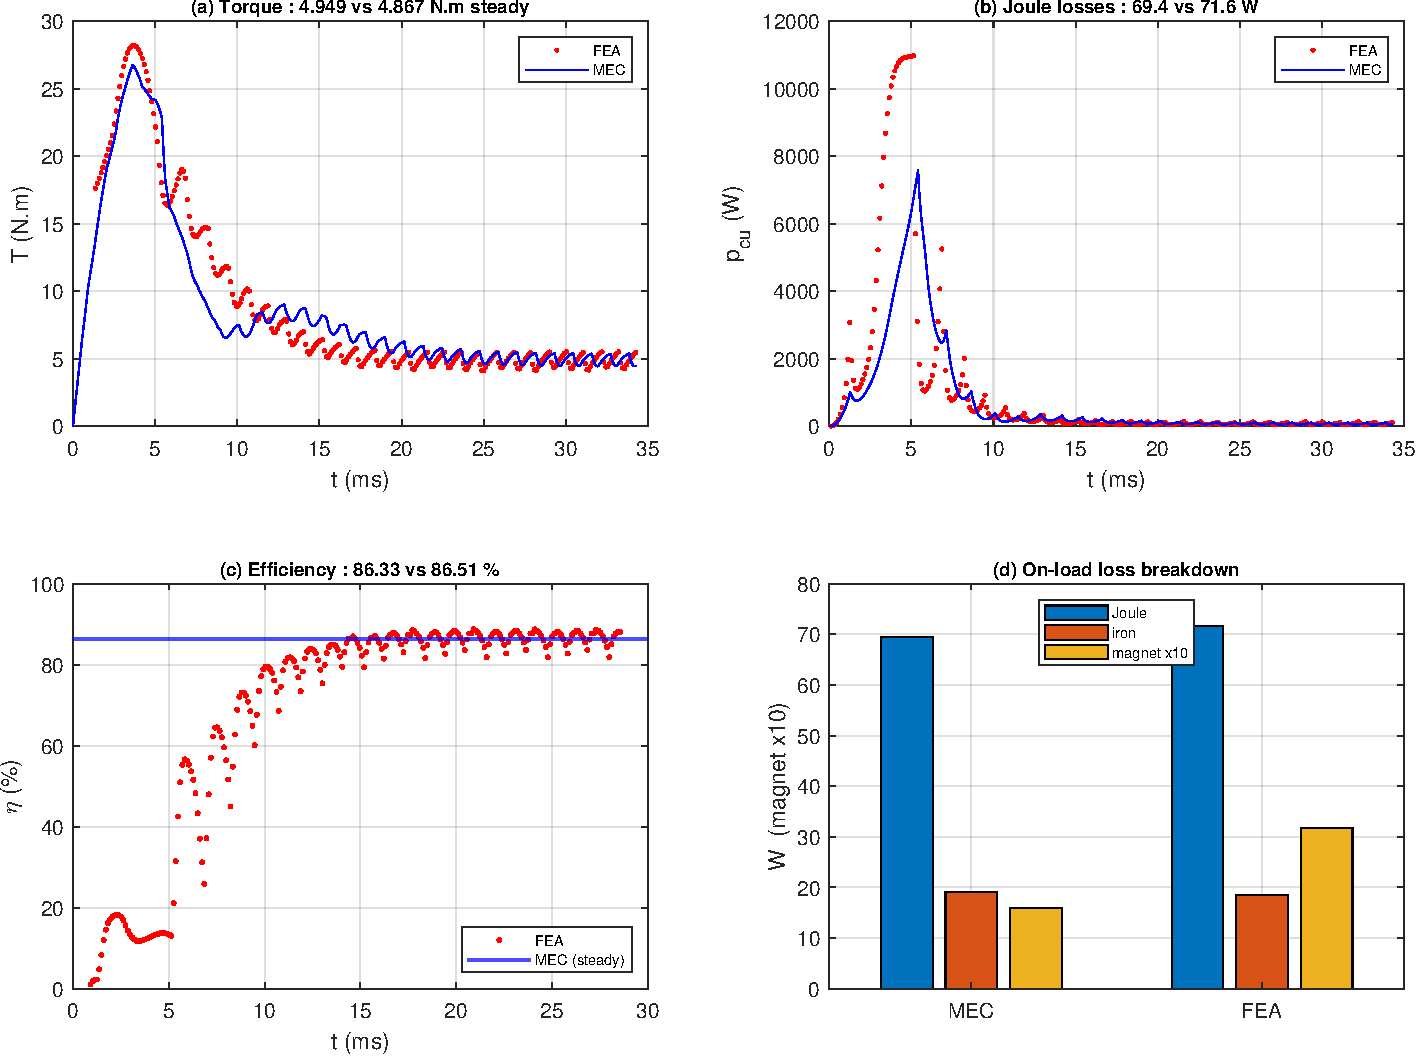
\includegraphics[width=\textwidth,height=0.44\textheight,keepaspectratio]{BLDC_FIG5_2_conversion.pdf}
\caption{On-load transient, conversion and losses, at the operating
point of Fig.~\ref{fig:load}. \textbf{(a)} Electromagnetic torque.
\textbf{(b)} Joule loss. \textbf{(c)} Efficiency. \textbf{(d)} Loss
breakdown by mechanism, which is what makes the efficiency
interpretable rather than merely reported.}
\label{fig:load_conv}
\end{figure*}







%=======================================================================


%======================================================================

\section{Comparison with Classical Air-Gap Closure Models}
\label{sec:closures}

Agreement with finite elements is necessary but not sufficient: the
formulation must also be shown to improve on the closure it replaces.
Table~\ref{tab:carter} isolates that comparison. Every row uses the
same one-branch-per-tooth iron network, at the same rotor position,
against the same reference; only the air-gap closure changes. This is
the closure axis of Fig.~\ref{fig:protocol}, and the refined mesh is
deliberately not used here.

\begin{description}[leftmargin=2.4em,style=sameline,font=\normalfont\bfseries]
\item[N1] \emph{smooth gap with Carter's factor}: the stator is replaced
by a smooth infinitely permeable surface and the geometric gap by
$g_{\mathrm{eff}}=k_{\mathrm{C}}g$, with $k_{\mathrm{C}}=\num{1.0100}$
computed on the magnetic gap $g'=g+h_{\mathrm{m}}/\murec$.
\item[N2] \emph{plus a generic permeance function}: the smooth field is
modulated by a relative permeance with a $\cos^2$ dip over the slot
opening.
\item[N2b] \emph{the permeance function of Silva} \emph{et
al.}~\cite{silva2023}, implemented as specified, a plateau followed by
a Gaussian decay, not a simple exponential, at three tangential
discretisations.
\item[N3] the proposed operator, the bore potential being carried by the
reluctance network.
\end{description}

The Carter value of row N1 is quoted in full so that the row can be
checked. With $b_0=\SI{2.000}{\milli\metre}$,
$g'=g+h_{\mathrm{m}}/\murec=\SI{4.3686}{\milli\metre}$ and a slot
pitch $\tau_{\mathrm{s}}=\pi D/N_{\mathrm{s}}
=\SI{14.5259}{\milli\metre}$, the \emph{exact} conformal-mapping form
\begin{equation}
\begin{aligned}
\gamma&=\frac{4}{\pi}\left[x\arctan x-\ln\sqrt{1+x^{2}}\right],
\qquad x=\frac{b_0}{2g'},\\[2pt]
k_{\mathrm{C}}&=\frac{\tau_{\mathrm{s}}}{\tau_{\mathrm{s}}-\gamma g'}
\end{aligned}
\label{eq:carter}
\end{equation}
gives $x=\num{0.22891}$, $\gamma=\num{0.033072}$ and
$k_{\mathrm{C}}=\num{1.010046}$. \emph{The exact form is the one used
here.} The approximate form in common design use,
$\gamma=(b_0/g')^{2}/(5+b_0/g')$, gives $\gamma=\num{0.038402}$ and
$k_{\mathrm{C}}=\num{1.011684}$ instead, a difference of
\SI{0.16}{\percent}. The choice is stated because the two are not
interchangeable at the precision of Table~\ref{tab:carter}.

\subsection{Construction of an Equitable Comparison}

An earlier version of this work compared the operator against N2 alone
and reported it overshooting the first sideband by \SI{307}{\percent}.
That was not a fair test of the family: the depth of a generic $\cos^2$
dip is not identified, and a closure judged on an unidentified parameter
is judged on nothing. Implemented as its authors specify, the same
family reaches \SI{-8.7}{\percent} on the first sideband, the
performance of the operator, which reaches \SI{-8.1}{\percent}. On that
row, and at that discretisation, N2b and N3 are indistinguishable.

The three N2b rows are what make the comparison informative, and they
are not a sensitivity study. The decay of a tooth-to-tooth permeance
function is parameterised by $\gamma_m$ and $\gamma_z$, which in
Ostovi\'c's construction are $|a_t-a_r|/2$ and $(a_t+a_r)/2$, where
$a_t$ and $a_r$ are the \emph{arcs of the elements} on the two surfaces.
\emph{Neither follows from the geometry of the machine.} They follow
from how the two surfaces have been discretised, so refining the
tangential mesh changes the permeance and with it the computed field.
Table~\ref{tab:carter} makes that dependence measurable: over three
tangential discretisations of the same machine, the first sideband
ranges from \SI{-96.4}{\percent} to \SI{+170.1}{\percent}, a spread of
\SI{219}{\percent}.

\emph{The argument therefore moves from accuracy to determination.} A
tooth-to-tooth permeance function is not less accurate than the
operator; it is undetermined, in the precise sense that the geometry
does not fix its parameters and the mesh does. The operator has no such
parameter to fix.

\subsection{Attributes Not Captured by Deviation Metrics}

N1 produces \emph{no} slot sideband whatsoever, an infinitely smooth
gap has no slot harmonic by construction, and underestimates the
tangential field by \SI{19.7}{\percent}; the residual $B_t$ it retains
comes from the transitions between magnets, not from slotting. And every
closure of the N1--N2b family returns the \emph{same} fundamental,
\SI{1.0958}{\tesla}. That equality is structural rather than
coincidental: a modulation whose period is the tooth pitch creates
harmonics only at orders $p\pm kN_{\mathrm{s}}$, so once normalised to
unit mean it leaves order $p$ untouched. The normalisation is verified
to six decimals for all four modulations. A permeance function modulates
the amplitude of a field it has not corrected, and the operator's
\SI{+0.3}{\percent} on the fundamental against \SI{+2.0}{\percent} for
the whole family is the measure of that difference.


%======================================================================

\section{Verification of the Finite-Element Reference}
\label{sec:audit}

A reduced-order model can only be validated against a reference whose
own uncertainty is known. This is rarely examined. The cogging torque of
the test PMSM provides a case in which the finite-element result, taken
at face value, would have condemned a correct model.
Fig.~\ref{fig:cog} sets out that case in four panels: panel~(a)
superimposes the two cogging curves on a common scale, panel~(b)
magnifies them over one slot pitch to show that both carry the same
erratic character, panel~(c) gives their spatial spectra, on which the
dominant order is the same in each, and panel~(d) isolates the physical
cogging that survives once the numerical content identified by the five
tests is removed. Five tests establish otherwise, and they generalise: none
requires the reference to be re-solved, which is the common situation
when a reduced-order model is validated against results supplied by a
third party.

\emph{The five tests are stated first as an instrument, independently of
this machine, because that is the form in which they are reusable.} Given
a reported quantity and nothing but the exports that accompany it, ask:

\begin{enumerate}[label=\textbf{T\arabic*.},leftmargin=*,itemsep=1pt]
\item \emph{Is it a periodic steady-state average?} A root-mean-square
over a window that does not span a whole period is not one, and the
signature is a ratio between phase and dc quantities that the conduction
pattern forbids.
\item \emph{Does its spectrum contain orders the geometry can support?}
An order that is not a multiple of the relevant least common multiple is
not the physical quantity, whatever its amplitude.
\item \emph{Do two meshing strategies of the same model agree?} A
preserved mesh and a regenerated one should differ by discretisation,
not by two orders of magnitude.
\item \emph{Is the residual, after removing the physical content,
consistent with mesh noise?} A surrogate built from the same spectrum
with randomised phases answers this without re-solving anything.
\item \emph{Does the quantity depend on a solver setting it should not
depend on?} If it does, the setting is a parameter and the quantity is
not a prediction.
\end{enumerate}

The instrument is applied below to the cogging torque of this machine,
where it changed the reading of one quantity, unfavourably to the
model.

\begin{figure*}[!tb]
\centering
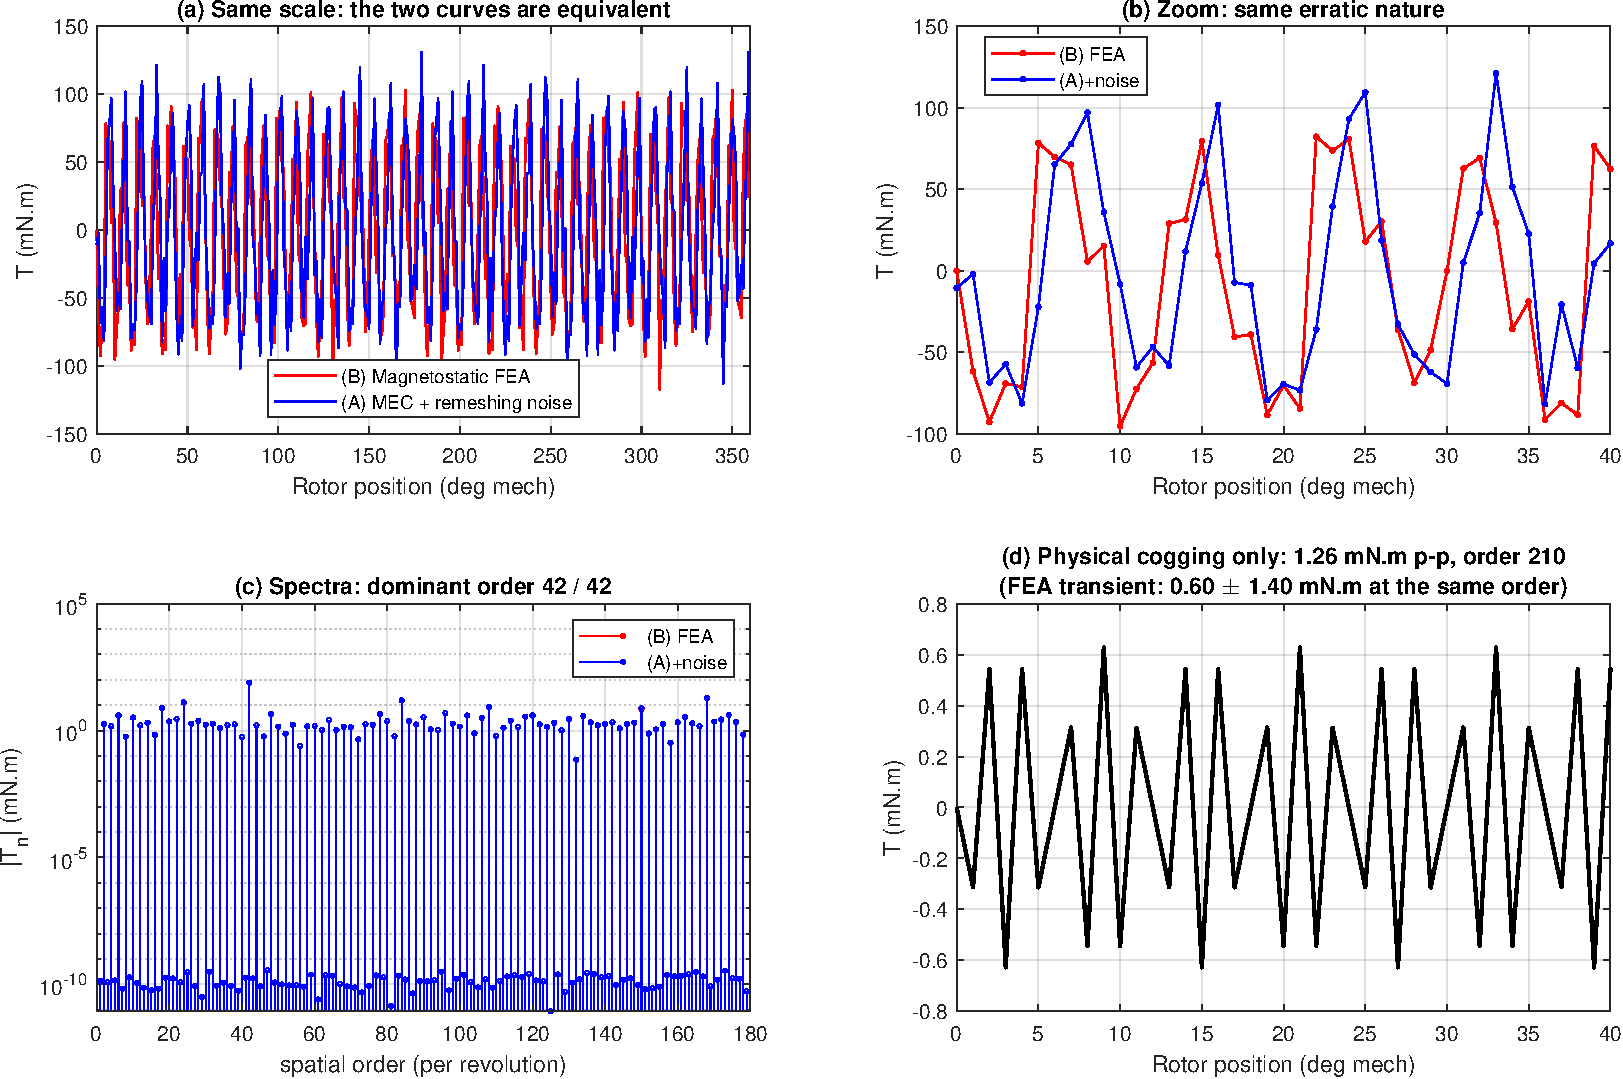
\includegraphics[width=\textwidth,height=0.44\textheight,keepaspectratio]{BLDC_FIG4_detente.pdf}
\caption{Cogging torque of the PMSM. \textbf{(a)} The two curves
superimposed on a common scale. \textbf{(b)} Magnification over one
slot pitch, showing that both carry the same erratic character.
\textbf{(c)} Spatial spectra, on which the dominant order is the same
in each. \textbf{(d)} The physical cogging that survives once the
numerical content identified by the five tests is removed.
The magnetostatic reference peaks
at order 42, which the 15/14 combination cannot contain; its residual is
shown to be remeshing noise by a surrogate with identical amplitude
spectrum. The physical cogging predicted by the model is
\SI{1.255}{\milli\newton\metre} peak-to-peak at order 210.}
\label{fig:cog}
\end{figure*}

\paragraph{Test 1 --- order rule.}
For a machine with $N_{\mathrm{s}}$ slots and $N_{\mathrm{m}}$ poles,
the cogging torque can only contain spatial orders that are multiples of
$\mathrm{lcm}(N_{\mathrm{s}},N_{\mathrm{m}})$. This rule is
classical~\cite{zhuhowe2000}; what is new here is to use it as a
\emph{falsification test on the reference} rather than as a design
guideline. Here the fundamental order is 210. The magnetostatic
reference peaks at order 42, which no cogging torque of a 15/14 machine
can contain. Table~\ref{tab:cog} makes the diagnosis quantitative:
\SI{90.1}{\percent} of the spectral energy of the reference lies at
multiples of $N_{\mathrm{m}}=14$ and \emph{none} at multiples of 210,
whereas the model places \SI{100}{\percent} at multiples of 210 and
nothing elsewhere. Energy at the pole number, and only at the pole
number, is the signature of a mesh regenerated once per magnet
position.

\begin{table}[!ht]
\centering
\footnotesize
\begin{threeparttable}
\begin{tabular}{@{}lrr@{}}
\toprule
 & Model & Reference\tnote{a} \\
\midrule
peak-to-peak amplitude (mN\,m)     & 1.255 & 220.2 \\
dominant spatial order             & \textbf{210} & \textbf{42} \\
amplitude at that order (mN\,m) & 0.628 & 77.07 \\
amplitude at order 210 (mN\,m)     & 0.628 & out of band \\
\midrule
\multicolumn{3}{@{}l}{\emph{Distribution of the spectral energy}}\\
multiples of 210 (physical)        & \SI{100.0}{\percent} & \SI{0.0}{\percent} \\
multiples of $N_{\mathrm{m}}=14$ only & \SI{0.0}{\percent} & \SI{90.1}{\percent} \\
multiples of $N_{\mathrm{s}}=15$ only & \SI{0.0}{\percent} & \SI{1.1}{\percent} \\
broadband                          & \SI{0.0}{\percent} & \SI{8.7}{\percent} \\
\midrule
angular Nyquist order              & 5866 & 180 \\
\bottomrule
\end{tabular}
\begin{tablenotes}[flushleft]\footnotesize
\item[a] Magnetostatic sequence, mesh regenerated at each position.
\end{tablenotes}
\end{threeparttable}
\caption{Harmonic comparison of the cogging torque: model against the
magnetostatic reference. Only multiples of
$\mathrm{lcm}(15,14)=210$ are physically admissible.}
\label{tab:cog}
\end{table}

\paragraph{Test 2, remeshed versus sliding band.}
The same machine solved with a preserved mesh gives
\SI{0.883}{\milli\newton\metre} at order 42, against
\SI{77.04}{\milli\newton\metre} when the mesh is regenerated at each
position: a ratio of \num{87.2}, attributable to the meshing strategy
alone, all other settings being identical.

Each amplitude must be read against the noise of \emph{its own} data
set, and the two are not the same. Writing
$\sigma=\operatorname{std}(r)\sqrt{2/N}$ for the standard error of a
spectral amplitude, the magnetostatic sequence
($N=360$ positions, mesh regenerated) has
$\sigma_m=\SI{1.950}{\milli\newton\metre}$ and the transient run
($N=101$, mesh preserved) has
$\sigma_t=\SI{0.340}{\milli\newton\metre}$. The order-42 component is
therefore $40\,\sigma_m$ in the first and $2.6\,\sigma_t$ in the second.
The two multiples are consistent with each other and with the amplitude
ratio, since $87.2=15.2\times5.73$ identically, the first factor being
the ratio of the multiples and the second that of the two standard
errors. A single symbol $\sigma$ for both data sets would make the same
numbers look contradictory, which is why both are named.

The verdict follows from the second data set alone: at
$2.6\,\sigma_t$ the order-42 component of the transient run lies below
$3\sigma_t=\SI{1.021}{\milli\newton\metre}$, that is, below its own
noise floor. Order 42 is not a physical component of this machine's
cogging torque; it is a property of the meshing strategy.

\paragraph{Test 3 --- angular Nyquist.}
At a \ang{1} step the Nyquist limit is order 180, so order 210 is not
representable; its alias would fall at 150, not at 42. The reference
does not even contain an aliased cogging component.

\paragraph{Test 4 --- energy balance.}
On the on-load transient, the dc-bus energy, the losses, the kinetic
energy and the load work close to within \SI{11.7}{\percent} over the
run and \SI{52.7}{\watt} in steady state, that is \SI{6.4}{\percent} of
the input. Any quantity smaller than that residual, the magnet loss is
\SI{3.18}{\watt}, cannot be resolved by the reference.

\paragraph{Test 4a, a positive confirmation.}
The four tests above are falsifications; a diagnosis is only complete
when the rejected data are also \emph{explained}. If the magnetostatic
curve is the sum of the physical cogging and a remeshing noise, then
adding a synthetic noise of the same amplitude spectrum to the computed
cogging must reproduce it. The residual $\Delta(\theta)$ between the two
curves is therefore replaced by a surrogate carrying its amplitude
spectrum with randomised phases, which shares its statistics but none of
its realisation. The outcome is unambiguous: standard deviation
\SI{60.56}{\milli\newton\metre} against \SI{60.53}{\milli\newton\metre},
order-42 amplitude \SI{77.07}{\milli\newton\metre} in both, dominant
order 42 in both, and the residual accounts for the variance of the
reference to within the resolution of the estimate
(\SI{100.1}{\percent}, i.e.\ statistically indistinguishable from
\SI{100}{\percent}). The magnetostatic curve is thus \emph{entirely}
explained as physical cogging plus mesh noise, with nothing left for a
model to predict.

The sign of the surrogate realisation is arbitrary, adding $\pi$ to
every phase yields the opposite noise with an identical amplitude
spectrum, so the realisation not in phase opposition with the reference
is retained. This is a presentation choice with no effect on any
statistic, and it is stated because the alternative would show two
visually anti-correlated curves that are in fact equivalent.

\paragraph{Test 5 --- averaging window.}
A fifth check applies to parametric sweeps, and it caught an
inconsistency that no convergence study would reveal. In the speed sweep
of Section~\ref{sub:drive_results}, the first point (\SI{10}{\rpm})
reports $\mathrm{rms}(i_a)=\SI{24.351}{\ampere}$ and
$\mathrm{avg}(i_{\mathrm{dc}})=\SI{24.352}{\ampere}$. For a \ang{120}
conduction pattern these two quantities differ by $\sqrt{2/3}$; their
equality can only mean that no commutation occurred within the
simulation window. Indeed the electrical period at that speed is
\SI{0.86}{\second}, far longer than the window. Whenever a sweep holds
its simulation time fixed while the electrical frequency varies by two
orders of magnitude, the low-speed points cannot be periodic
steady-state averages. The test costs nothing, it compares two numbers
already present in the output, and it identifies which points of a
published characteristic may be used for validation.

\subsection{Cogging-Torque Outcome of the Verification Tests}

Applying these tests, the admissible reference for cogging is the
transient run with a preserved mesh: \SI{0.604}{\milli\newton\metre}
peak-to-peak with a $2\sigma$ uncertainty of
\SI{1.401}{\milli\newton\metre}, at order 210. \emph{The two dispersions
quoted in this section are not the same statistic and must not be
compared directly}: $\sigma_t=\SI{0.340}{\milli\newton\metre}$ above is
the per-sample standard deviation of the torque waveform, whereas
\SI{1.401}{\milli\newton\metre} is a $2\sigma$ interval on the
\emph{peak-to-peak} amplitude, which is the quantity being compared.
The ratio of the two,
$\num{1.401}/(2\times\num{0.340})=\num{2.06}$, is formed from the two
figures above; the propagation that would produce it is not established
here and the two statistics are reported separately for that reason.
The lumped model predicts
\SI{1.255}{\milli\newton\metre} at exactly that order, a difference of
\SI{0.651}{\milli\newton\metre}.

The correct reading of this agreement is a non-rejection, not a
validation, and the point should be made explicitly: with a $2\sigma$ interval of
\SI{1.401}{\milli\newton\metre}, any prediction below roughly
\SI{2}{\milli\newton\metre}, including zero, would be equally
compatible with the reference. The reference has no resolving power on
this amplitude. The result that does carry information is the
\emph{order}: 210 is predicted from theory before any computation, and
the computed spectrum peaks there and nowhere else. Only the amplitude
is computed, and only the amplitude is unresolved.

The magnitude of the contamination can be referred to a quantity the
paper does validate. Converted to an equivalent perturbation of the
radial flux density, the remeshing noise of the magnetostatic sequence
corresponds to about \SI{0.0047}{\tesla}, against
\SI{0.0197}{\tesla} for the first slot sideband measured on the same
reference: that is, \SI{24}{\percent} of the very harmonic the model is
being asked to reproduce. The mesh convergence of the reference is
therefore not established at the amplitude of the quantities in
question, which is the substance of the recommendation made in
Section~\ref{sec:bounds}.

\subsection{Uncertainty Budget of the Reference Solution}

Tests~2 and~4 are not merely diagnostics; together they constitute a
quantitative sensitivity study of the reference, obtained without
re-solving it. Test~2 is a \emph{meshing-strategy} sensitivity in the
strict sense: two runs of the same machine, at the same operating point,
with the same material data, differing only in whether the mesh is
regenerated at each rotor position or transported by a sliding band. The
spread between them, a factor of 87 on the order-42 component, bounds
the discretisation uncertainty of the reference on the cogging torque
far more sharply than a conventional mesh-density study would, because
it isolates the mechanism responsible rather than a global element
size.

Test~4 bounds the reference on power quantities. The steady-state
residual of \SI{52.7}{\watt}, \SI{6.4}{\percent} of the input power,
sets the resolution floor of that finite-element run.
Table~\ref{tab:unc} places the model--reference deviations against it.
Quantities whose deviation exceeds the floor by a wide margin are
genuine model errors; quantities of the same order as the floor cannot
be resolved by the reference and must be reported as such. The on-load
magnet loss falls in the second category: it represents
\SI{0.4}{\percent} of the input power, below the residual of the run
that measures it.

\begin{table}[!ht]
\centering
\footnotesize
\begin{tabular}{lrl}
\toprule
Quantity & deviation & vs.\ floor \\
\midrule
copper loss                 & \SI{-1.5}{\watt} & below \\
iron loss                   & \SI{+0.6}{\watt} & below \\
magnet loss, on load        & \SI{-1.6}{\watt} & below \\
electromagnetic power       & \SI{+15}{\watt}  & below \\
efficiency                  & $-0.2$ p.p.      & --- \\
\midrule
\textbf{resolution floor}   & \SI{52.7}{\watt} & --- \\
\bottomrule
\end{tabular}
\caption{PMSM model deviations placed against the resolution floor of
the reference, from Test~4.}
\label{tab:unc}
\end{table}

A conventional mesh-density refinement of the reference would refine
this budget further and is recommended whenever the finite-element
project can be re-solved. The five tests above are designed for the case
in which it cannot, and we propose them as a routine check before any
reduced-order model is validated on finite-element cogging or
small-signal loss data.

%=======================================================================

%======================================================================

\section{Limitations and Bounds of Validity}
\label{sec:bounds}

\subsection{The Tooth-Tip Corner Singularity}
\label{sub:corner}

Two quantities do not converge with mesh refinement: the first slot
sideband and the cogging torque. Section~\ref{sub:conv} shows why, and
the demonstration rests on the two refinement directions disagreeing
rather than on a single sequence failing to settle. Refining the bore
angularly raises the sideband; refining the shoe radially lowers it; and
under the linear solver the peak iron flux density grows from
\SI{2.80}{\tesla} to \SI{3.47}{\tesla} on a material that saturates near
\SI{2}{\tesla}. There is a singularity, and it is not introduced by the
network: the tooth tip is a sharp corner in the reference model itself,
the fillet being applied inside a boolean block. The field there
diverges, and the computed value depends on the cell size at the
corner, in the network as in the finite-element mesh.

The direction of the shift between the linear and nonlinear solutions is
physical. Saturating the tooth-tip corners lowers their permeability,
deepens the air-gap permeance dip under the slot opening and therefore
strengthens the slot modulation. A linear model cannot produce this and
necessarily underestimates; Newton produces it and overshoots. The
correct statement is a bracket rather than a value,
\begin{equation}
\underbrace{0.01596}_{\text{linear}} <
\underbrace{0.01966}_{\text{FEA}} <
\underbrace{0.02434}_{\text{Newton}}\ \si{\tesla},
\label{eq:bracket}
\end{equation}
in which the reference is itself a mesh-dependent quantity. Both bounds
come from the $M_{\mathrm{s}}=900$ row of Table~\ref{tab:convb} and
therefore from a single execution.

The bracket does not close. Its width, measured between the same two
solvers at the same angular grid, is \num{41.7} percentage points at one
layer per shoe sub-region and \num{42.6} at four: refining the very
region that should resolve the quantity leaves the two predictions as
far apart as before. That is the operational content of the word
singular, and it is why we recommend reporting the slot sideband as an
indicator of corner resolution rather than as a validated output, for
the network and for the finite-element model alike.

One consequence of this must be stated before it is noticed elsewhere,
because it looks like a defeat and is not. On the first slot sideband
the \emph{lumped} network is the closest of the three models to the
reference---\SI{-8.1}{\percent} against \SI{-13.3}{\percent} for the
refined mesh at one shoe layer and \SI{-19.6}{\percent} at two
(Table~\ref{tab:pmsm}). The coarser iron model wins on this row. Given
what precedes, that is expected rather than embarrassing: the quantity
is singular, its computed value is set by the cell size at the corner,
and a model with one cell there has no more claim to the right answer
than a model with eight, it simply happens to land nearer. Reporting
that proximity as an accuracy result would be reporting an accident, and
it is the reason the sideband is quoted as a bound throughout this paper
instead of as a validated output. The same caution applies to the
comparison of Section~\ref{sec:closures}, which is conducted on the
lumped iron model by design and whose sideband figures inherit this
status.

The recommendation extends, with more force, to the second slot
sidebands. Table~\ref{tab:spectrum} shows the network overshooting the
reference by \SI{61}{\percent} at $\nu=23$ and \SI{58}{\percent} at
$\nu=37$, against \SI{8}{\percent} at $\nu=8$ and $\nu=22$. The ordering
is what the singularity argument predicts: the angular wavelength of the
second sidebands is about half the slot opening, so they sample the
corner region where the field diverges more sharply than the first
sidebands do, and the discretisation error there is correspondingly
larger. No mesh refinement removes this, in the network or in the
reference, because neither resolves a divergent field. Any use of the
model that depends on orders above the first sidebands, acoustic noise
prediction being the obvious one, requires a corner treatment that this
formulation does not provide.

\subsection{A Single Defect Observed Through Two Projections}
\label{sub:unity}

The corner singularity and the harmonic tail of Section~\ref{sec:trace}
are not two separate limitations. They are the same defect of regularity
seen in two bases.

In the Fourier basis, a piecewise-constant bore potential is
discontinuous, its coefficients decay as $1/n$, and the energy sum
diverges logarithmically---Proposition~1. In the mesh basis, the field
at a re-entrant corner behaves as $r^{\lambda-1}$ with $\lambda<1$, so
the flux through the cell adjacent to the tip depends on the cell size
and no refinement settles it. The exponent is not an empirical
observation: for the scalar potential on a wedge of interior angle
$\omega>\pi$ the leading singular exponent is $\lambda=\pi/\omega$,
which for the re-entrant angle of a tooth tip lies strictly below
unity~\cite{grisvard1985}; the electromagnetic form of the same
statement is the classical edge condition~\cite{meixner1972}. Both statements say that the solution does
not lie in the space in which the discrete problem is being posed, and
both have the same consequence: quantities that integrate the field over
a whole tooth converge, quantities concentrated at the tip do not.

The two also differ in one respect that matters for practice, and it is
the reason Section~\ref{sec:trace} exists. The harmonic tail is a defect
of the \emph{trial space}, and changing the trial space removes it: the
hat basis restores an absolutely convergent series at the cost of one
line of code. The corner singularity is a defect of the \emph{solution},
present in the reference as much as in the network, and no change of
basis removes it. One is repairable, the other is to be reported.

\subsection{Which Geometries the Locking Protects, and Which It Does Not}
\label{sub:generality}

The preceding subsections concern this machine. The mechanism they rest
on is geometric, so it can be turned outward, and the criterion is
explicit: the harmonic tail installs itself once $n\gtrsim1/\Ua$, where
$\Ua$ is the logarithmic thickness of the \emph{air} layer of the
annulus being condensed, not of the annulus as a whole, since a magnet
layer of recoil permeability near unity does not enter the degeneracy.
Here $\Ua=\num{0.02926}$ and the tail begins near $n\approx34$; on the
doubly slotted gap of Appendix~\ref{app:im} the annulus is bare air,
$\Ua=\Xg=\num{2.97e-3}$, and it begins near $n\approx337$. \emph{The thin-gap machine is therefore the
protected one over any truncation a designer would use}, and the thick
annulus of a surface-magnet rotor is the exposed one, which is the
opposite of the intuition that a thicker air path is more forgiving, and
the reason Section~\ref{sub:v1} insists that thickness is not the
immunity mechanism.

What protects the present machine is not its geometry but the rank
condition $N=\lfloor M_{\mathrm{s}}/2\rfloor$, which locks the
truncation to the tiling and holds the divergent bracket stationary
at $\ln\pi$. That locking is a property of \emph{this chain}, not of the
formulation: any implementation that lets $N$ be chosen independently of
$M_{\mathrm{s}}$, as a Schur condensation onto the tooth nodes
does, loses it immediately. The criterion for a new machine is therefore twofold: form
$\Xg$ to locate the tail, and check whether the truncation is free of
the tiling. A machine with a thick magnet layer, a fine surface grid and
a freely chosen truncation is the case in which the defect would be
visible in the outputs rather than only in the operator.

\subsection{Magnet Losses: Distribution of a Single Deviation}
\label{sub:pmloss_bound}

An earlier version of this work presented the magnet losses as a
dichotomy: a no-load point validating the whole chain within
\SI{2.4}{\percent}, and an on-load point left open at
\SI{-50}{\percent}. Neither figure survives regeneration, and the
dichotomy does not exist.

The no-load value on which the \SI{2.4}{\percent} rested was produced by
a second routine, and that routine carried a sign error in its
transformation to the rotor frame; Section~\ref{sub:pmloss} gives the
test that exposes it and the correction. Corrected, it returns
\SI{-36.4}{\percent} on the same point, beside the \SI{-39.1}{\percent}
the frozen chain gives from the one-branch-per-tooth field and the
\SI{-24.7}{\percent} it gives from the polar mesh. \emph{The agreement
claimed at no load rested on one sign.}
The on-load comparison, for its part, was formed between two runs at
different operating points, \SI{1257}{\rpm} against
\SI{1340}{\rpm} and \SI{1.419}{\ampere} against
\SI{1.552}{\ampere}. Eddy-current loss scales as $\omega^2$ and as the
square of the exciting current, so the two runs differ by a factor
$(1257/1340)^2(1.419/1.552)^2=\num{0.736}$ before any modelling error is
invoked. Normalised to a common operating point, the on-load deviation
is \SI{-32.6}{\percent}.

The four deviations are therefore \SI{-36}{\percent},
\SI{-39}{\percent}, \SI{-25}{\percent} and \SI{-33}{\percent}: one
deviation of a single order, distributed differently according to the
operating point and the source of the field, rather than two
qualitatively distinct situations. That is a weaker claim than the one
it replaces, and a true one, and it now rests on four figures that
agree instead of on three and an outlier. What remains reportable is
the fourteen points that separate the two field sources at no load,
which is the measurable contribution of the mesh to this quantity.

The magnitude should be read against Section~\ref{sec:audit}: the
on-load magnet loss is \SI{0.4}{\percent} of the input power, below the
\SI{6.4}{\percent} energy-balance residual of the reference run that
measures it. The reference cannot resolve the quantity on which it is
being compared.

\subsection{Integral Quantities and the Loss Exception}
\label{sub:integral}

Four rules follow for the use of the method, and the third is a
restriction of a claim made in the earlier version of this work.

\paragraph{First, integral quantities are the ones the method predicts
reliably.}
Flux linkage, back-electromotive force, inductances and mean torque
integrate the field over a whole tooth and are insensitive to the
corner. Section~\ref{sec:pmsm} confirms it: within \SI{0.35}{\percent}
on flux linkage and self-inductance, \SI{0.10}{\percent} on the
synchronous inductance, without a single fitted air-gap constant, all
three on the refined mesh, and the last of them a difference of two
errors of opposite sign, \SI{0.33}{\percent} when the reference mutual
inductance is used instead. On the lumped model, which is what every
other result of Section~\ref{sec:pmsm} uses, the same three quantities
are \SI{1.11}{\percent}, \SI{1.12}{\percent} and \SI{1.24}{\percent}.

\paragraph{Second, local quantities must be reported as bounded.}
Slot sidebands, cogging torque, and any quantity built from them must
carry the solver and the corner discretisation used. This applies
equally to a finite-element reference.

\paragraph{Third, losses belong with the local quantities, and the
reason is not the one that might be assumed.}
The earlier version placed losses among the integral quantities, on the
grounds that a loss is an integral over a volume. The regeneration shows
that the classification must follow the \emph{convergence} of the
quantity rather than its form, and the two do not agree here.

The evidence is threefold and each piece says something different. The
magnet loss moves by fourteen points---from \SI{-39.1}{\percent} to
\SI{-24.7}{\percent}, according to the source of the field alone. The
iron loss moves from \SI{+15.3}{\percent} to \SI{+25.3}{\percent} for
the same reason. And under refinement of the shoe at a fixed field
source, the \emph{total} iron loss drifts by only \SI{1.86}{\percent}
while the share carried by the shoe cells drifts by
\SI{20.28}{\percent}.

That last figure is the one that settles the classification. A loss is
the sum of a volumetric part, which converges, and a corner part, which
does not. Here the corner part carries \SI{10}{\percent} of the total,
so the total looks robust, but that is a property of how the losses are
distributed \emph{in this machine}, not a guarantee. On a machine whose
shoe carries more of the loss, higher frequency, thinner shoe, deeper
saturation: the same defect would dominate the total. It would be wrong
to write that losses drift like the slot sideband, which doubles over
the same sweep; and equally wrong to call them integral because their
total happens to be stable.

One observation completes the picture and guards against a false
reassurance. Under the Newton solver the peak iron flux density stays
between \SI{1.974}{\tesla} and \SI{1.979}{\tesla} as the shoe is refined
from one layer to four at $M_{\mathrm{s}}=540$, and it would be natural
to read that as convergence. It is not. Under the linear solver the same
corner diverges from \SI{2.80}{\tesla} to \SI{3.47}{\tesla} on the shoe
sweep at $M_{\mathrm{s}}=900$ (Section~\ref{sub:conv}).
\emph{Saturation bounds the amplitude of the field at the corner without
removing its dependence on the mesh}, and a bounded quantity is not
therefore a converged one.

\paragraph{What is not modelled at all, as distinct from what is
modelled and bounded.}
The rules above concern quantities the model computes. Three loss
mechanisms it does \emph{not} compute should be named so that the loss
budget is not read as complete: rotor iron loss, axial segmentation of
the magnets, and end effects, end-winding leakage beyond the analytical
term, and the axial variation of the field at the stack ends. None
appears in \eqref{eq:pmloss} or in the Bertotti summation, and none is
bounded here. A two-dimensional formulation cannot address the last of
them at all.

\paragraph{What the method is now good for.}
The rules above are stated negatively, and the positive statement is
owed to the reader. On the evidence of this paper, integral quantities
within \SI{0.35}{\percent} on flux linkage and self-inductance without a
fitted air-gap constant, and a complete eight-analysis study in
\SI{133}{\second}, the formulation is suitable for no-load design
iteration, for back-electromotive-force and inductance prediction, and
for magnet sizing. It is \emph{not} suitable, on the same evidence, for
acoustic-noise prediction, for cogging-torque design, or for drive
operating-point prediction: the first two rest on the slot sidebands and
the cogging spectrum, which Section~\ref{sub:corner} shows are governed
by the corner singularity and reported as bounds, and the third is the
subject of the \SI{25.4}{\percent} deficit of
Section~\ref{sub:drive_results}.

\paragraph{Fourth, and as a consequence of Section~\ref{sec:audit}.}
When the reference and the model disagree on a quantity smaller than the
reference's own energy-balance residual, the disagreement carries no
information. Section~\ref{sec:audit} makes that residual measurable
without re-solving the reference; we recommend computing it before
attributing any discrepancy to the model.

%======================================================================

\section{Conclusion}
\label{sec:conclusion}

Replacing the empirical air-gap permeance of a magnetic equivalent
circuit by the exact Dirichlet-to-Neumann operator of the annulus
removes the last non-predictive element of the method. The operator
spans two layers, air and magnet, and carries the magnetisation as a
source inside a single surface map, so the magnet region needs no
separate matching. It is symmetric and negative semi-definite, its null
space being the constant potential, so the coupled system is well posed
once the iron network fixes the gauge. Where the inner boundary is
smooth it is invariant with rotor position, and a sweep of \num{721}
positions then costs one factorisation and \num{721}
back-substitutions.

The central result of this paper concerns not the operator but its
condensation. A reluctance network carries one potential per node, so
the natural trial space on the bore is piecewise constant, and a
piecewise-constant function does not belong to $H^{1/2}$, the trace
space on which the Dirichlet-to-Neumann map is bounded. The consequence
is not a loss of accuracy but a loss of definition: we prove in closed
form that the self-energy of a bore column grows as
$\ln N$ without bound, verify the closed form to $1.4\times10^{-6}$ over
four decades, and recover the predicted slope $2\mu_0L/\pi\cdot\ln 10$
to four significant figures at three column widths, with no adjusted
quantity anywhere. \emph{Under a piecewise-constant projection, the
condensed operator has no limit; the truncation selects a value rather
than approximating one.} The continuous piecewise-linear basis belongs
to the trace space, restores an absolutely convergent series with a
residual tail in $1/N^{2}$, and costs one line of code.

That result is not specific to electrical machines. It applies to any
condensation of a surface operator onto a discontinuous basis, and the
diagnostic that reveals it, the ratio of successive increments, tending
to unity for a logarithmic tail and to a constant below one for a
geometric one, is available to anyone who can run the same sum twice.

The formulation is validated against two-dimensional finite elements on
a \SI{750}{\watt} 15-slot/14-pole surface-mounted PMSM, in a single
declared configuration rather than row by row. The synchronous
inductance agrees within \SI{0.10}{\percent}, the self-inductance within
\SI{0.34}{\percent}, the flux linkage within \SI{0.24}{\percent} and the
fundamental air-gap flux density within \SI{0.31}{\percent}, three
previously fitted constants having been removed. Two of these figures
carry a stated reservation: the synchronous inductance is a difference
of two quantities whose errors subtract, and with the reference mutual
inserted it would read \SI{0.33}{\percent}; and refining the shoe moves
thirteen of the seventeen quantities away from the reference instead of
towards it, which is the integral counterpart of the corner singularity
and the reason both columns are reported as a bracket.

The price is stated rather than hidden. The same transient that yields
the efficiency agreement settles at a speed low by \SI{6.2}{\percent},
and the speed sweep runs \SI{25.4}{\percent} low on peak power: the loss
structure is reproduced, the operating point is not. The deviation is
located instead of merely reported, the mean absolute deviation on
torque per ampere being \SI{15.1}{\percent} against \SI{25.8}{\percent}
on torque, which places
the error in the current instead of in the electromagnetic conversion.

Against the closure it replaces, the comparison was made fair before it
was made. Implemented as its authors specify, a tooth-to-tooth permeance
function reaches the operator's accuracy on the first slot sideband.
What separates them is not accuracy but determination: its two shape
parameters are arcs of mesh elements rather than dimensions of the
machine, and over three tangential discretisations of the same geometry
the first sideband spans \SI{219}{\percent}. The operator has no
parameter of that kind to fix.

The paper also delimits what the method does not do, and the
delimitation is a result. The first slot sideband and the cogging torque
are governed by a tooth-tip corner singularity; they are bracketed by
the two solvers, the bracket does not close under refinement of the very
region that should resolve it, and they are reported as bounds. That
defect and the harmonic tail are the same failure of regularity seen in
two bases, one repairable by changing the trial space, the other
present in the reference as much as in the network. Losses are excluded
from the integral-quantity rule for a reason that had to be measured
rather than assumed: their total can look stable while their corner
share drifts by \SI{20}{\percent}, and saturation bounds the amplitude
of the corner field without removing its dependence on the mesh.

Finally, the five-test procedure proposed for auditing the
finite-element reference is, in our view, as reusable as the formulation
itself. On this machine it establishes that the magnetostatic cogging
reference peaks at a spatial order the slot--pole combination cannot
contain, that two meshing strategies of the same model differ by a
factor of \num{87} on that order, and that the residual is entirely
accounted for as physical cogging plus mesh noise, with nothing left for
a model to predict. A reduced-order model cannot be more accurate than
the reference against which it is measured, and that reference is not
always what it appears to be.

\subsection*{Further work}
\label{sub:further}

Three items follow directly and in order of priority. The first is the
experiment that Section~\ref{sub:v1} identifies but does not perform:
unlocking the truncation from the tiling on the permanent-magnet chain.
That chain imposes $N=M_{\mathrm{s}}/2$ for a reason unrelated to
convergence, the rank of the bore operator, and \eqref{eq:lock} shows
that the constraint holds the divergent term stationary. Condensing the
bore by a Schur complement, as a doubly slotted annulus requires,
would free the truncation and make the drift observable on
this machine as well; the prediction of Section~\ref{sub:p0closed} is
then quantitative and falsifiable. The second is a corner treatment for
the tooth tip, a graded mesh, a singular enrichment or a fillet
resolved on both sides, without which the slot sidebands remain bounds
in the network and in the reference alike. The third is a controlled
timing comparison of the two methods on identical hardware and to a
common accuracy target on a named quantity, together with the two
open-circuit measurements of Section~\ref{sub:posture} on a prototype. The last of
these is necessary before the model is used for absolute performance
prediction; it is not required by, and is not claimed for, the
formulation result presented here.

%======================================================================

\appendix

\section{The Doubly Slotted Geometry Used in Sections~\ref{sec:trace} and~\ref{sub:v1}}
\label{app:im}

\emph{Declared overlap.} This geometry is also the subject of a companion
manuscript submitted concurrently by the present authors, which treats
the doubly slotted operator in its own right and applies
Proposition~\ref{prop:closed} to it. It is used here only as the thin
annulus on which the divergence of Proposition~\ref{prop:closed} is
observable, and no result of that paper is assumed anywhere in this one.
The overlap is confined to the dimensions listed below.

Two results of this paper are computed on the air gap of an
\SI{18.5}{\kilo\watt} 48-slot/44-bar cage induction machine rather than
on the permanent-magnet machine validated here, because the thin-annulus
regime is where the divergence is observable. The geometry is stated in
full so that both can be reproduced from this paper alone.

The annulus is bounded by two slotted iron surfaces. Stator bore
$\Rs=\SI{81.8888}{\milli\metre}$, rotor outer radius
$\SI{81.6458}{\milli\metre}$, hence a mechanical gap
$g=\SI{0.2430}{\milli\metre}$ and a logarithmic thickness
$\Xg=\ln(\Rs/R_{\mathrm{r}})=\num{2.9719e-3}$, a factor of \num{46.8}
below the \num{0.13899} of the machine of Section~\ref{sec:pmsm} and a
factor of \num{9.85} below the \num{0.02926} of its air layer taken
alone, which is the thickness that governs the spectral tail of
Section~\ref{sub:v1}. There
are 48 stator slots and 44 rotor bars on an active length
$L=\SI{164.7824}{\milli\metre}$, both slot openings being
\SI{2.000}{\milli\metre}, so that the slot pitches are
$\tau_{\mathrm{s}}=\SI{10.7192}{\milli\metre}$ and
$\tau_{\mathrm{r}}=\SI{11.6590}{\milli\metre}$ and the opening-to-gap
ratio is \num{8.23} on both surfaces.

Table~\ref{tab:p0tail} uses these dimensions with the degenerate
kernel. The upper panel of Table~\ref{tab:v1basis} uses the full
condensed operator of the same annulus, assembled as follows: both bores
are tiled by $n_T$ columns spanning each tooth face and $n_O$ columns
spanning each slot opening, so that the columns pave the two surfaces
exactly; the operator is built on that fine grid, where the Laplace
solution of the annulus is exact; and the opening columns, which deliver
no flux into iron, are eliminated by a Schur complement onto the tooth
nodes. No fringing coefficient enters. Only the increments of the
resulting reactance are used in this paper, and they are those of
Table~\ref{tab:v1basis}.




%======================================================================
\section{The Twenty-Nine Compared Quantities}
\label{app:scorecard}

Section~\ref{sub:stats} states that the comparison set is reported in
full, and Fig.~\ref{fig:score} synthesises it as twenty-nine bars. The
values behind those bars are collected here so that both counts the
figure carries can be checked one line at a time.

\begin{table*}[!t]
\centering
\begin{threeparttable}
\footnotesize
\setlength{\tabcolsep}{5pt}
\begin{tabular}{@{}rllrrrc@{}}
\toprule
\# & quantity & unit & network & reference & deviation & \\
\midrule
1 & $B_{g1}$ fundamental & T & \num{1.07755} & \num{1.07455} & $+0.28\%$ & \\
2 & $|B_r|$ mean & T & \num{0.761473} & \num{0.760909} & $+0.07\%$ & \\
3 & $B_r$ peak & T & \num{0.984576} & \num{0.990727} & $-0.62\%$ & \\
4 & $B_t$ rms & T & \num{0.143165} & \num{0.133238} & $+7.45\%$ & $\star$\\
5 & flux line $A$, peak & Wb/m & \num{0.00585972} & \num{0.00585343} & $+0.11\%$ & \\
6 & MMF per magnet, mean & A & \num{763.243} & \num{769.445} & $-0.81\%$ & \\
7 & MMF per gap, mean & A & \num{723.829} & \num{721.504} & $+0.32\%$ & \\
8 & MMF per magnet, dispersion & \% & \num{6.80730} & \num{6.58458} & $+3.38\%$ & \\
9 & reluctance factor $k_{\mathrm{r}}$ & --- & \num{1.05445} & \num{1.08693} & $-2.99\%$ & \\
10 & leakage factor $k_{\mathrm{l}}$ & --- & \num{0.853766} & \num{0.867230} & $-1.55\%$ & \\
11 & self inductance $L_{\mathrm{a}}$\tnote{c} & mH & \num{50.8159} & \num{50.2086} & $+1.21\%$ & \\
12 & mutual inductance $M$\tnote{c} & mH & \num{-2.22152} & \num{-2.13292} & $+4.15\%$ & \\
13 & synchronous inductance $L_{\mathrm{d}}$\tnote{c} & mH & \num{53.0374} & \num{52.3415} & $+1.33\%$ & \\
14 & phase back-EMF, peak & V & \num{240.936} & \num{233.031} & $+3.39\%$ & \\
15 & six-step envelope, peak & V & \num{469.262} & \num{459.918} & $+2.03\%$ & \\
16 & flux linkage, peak & Wb & \num{0.261206} & \num{0.258328} & $+1.11\%$ & \\
17 & torque, on load & N\,m & \num{4.94901} & \num{4.86664} & $+1.69\%$ & \\
18 & phase current, rms & A & \num{1.41857} & \num{1.55162} & $-8.58\%$ & $\star$\\
19 & iron loss, no load & W & \num{21.3358} & \num{19.7298} & $+8.14\%$ & $\star$\\
20 & magnet loss, no load\tnote{a} & W & \num{0.212037} & \num{0.333466} & $-36.41\%$ & $\star$\\
21 & steady-state speed, on load & rpm & \num{1257.030} & \num{1339.830} & $-6.18\%$ & $\star$\\
22 & dc-bus current, mean & A & \num{1.42741} & \num{1.65746} & $-13.88\%$ & $\star$\\
23 & iron loss, on load & W & \num{19.0830} & \num{18.4650} & $+3.35\%$ & \\
24 & magnet loss, on load\tnote{a} & W & \num{1.57752} & \num{3.18268} & $-50.43\%$ & $\star$\\
25 & efficiency, on load & \% & \num{86.3340} & \num{86.5148} & $-0.18$ p.p. & \\
26 & back-EMF constant $k_E$ & mV/rpm & \num{312.841} & \num{323.644} & $-3.34\%$ & \\
27 & standstill torque (sweep)\tnote{b} & N\,m & \num{30.6807} & \num{29.2331} & $+4.95\%$ & \\
28 & peak power (sweep) & W & \num{1115.070} & \num{1495.270} & $-25.43\%$ & $\star$\\
29 & peak efficiency (sweep) & \% & \num{85.4456} & \num{89.4319} & $-3.99$ p.p. & \\
\bottomrule
\end{tabular}
\begin{tablenotes}[flushleft]\footnotesize
\item[a] Magnet loss, declared in Section~\ref{sub:pmloss_bound} as not
validated: the reference cannot resolve the quantity being compared.
\item[b] Standstill torque, excluded from the comparison in
Section~\ref{sub:eligibility}.
\item[c] The three inductance rows are solved at $\mu_{\mathrm{r}}=5000$;
every other row of this table is solved at $\mu_{\mathrm{r}}=3000$. The
two values are declared here because they differ, and because
Table~\ref{tab:pmsm} uses \num{3000} throughout. \emph{The figure quoted
in the abstract and in Table~\ref{tab:pmsm} for the lumped synchronous
inductance is the one at $\mu_{\mathrm{r}}=3000$, \SI{+1.24}{\percent},
which is the setting used everywhere else in this paper}; the
\SI{+1.33}{\percent} of row~13 is the same quantity at
$\mu_{\mathrm{r}}=5000$. A reader meeting either figure first should be
able to find the other, which is why both are named here, see also the
note below.
\item $\star$ marks a deviation of \SI{5}{\percent} or more. Eight of the
twenty-nine are so marked, so twenty-one fall within the threshold;
excluding the three declared not validated, of which two are outside it,
the count is twenty of twenty-six.
\item \emph{Configuration.} One execution of the lumped-iron chain, the
one that produces Fig.~\ref{fig:score}: \num{721} rotor positions, the
field evaluated at the position registered on the finite-element
solution. Sixteen of these quantities also appear in
Table~\ref{tab:pmsm}, which is a \emph{different} configuration, \num{61}
rotor positions, the field at $\varphi=0$, and
$\mu_{\mathrm{r}}=\num{3000}$ on the inductances as well. The two agree
to \SI{0.21}{\percent} or better on all sixteen, and neither is adjusted
to match the other: a fundamental is invariant under rotation and
coincides exactly, a peak is not and does not. \emph{Each table reports
one chain, and says which.}
\end{tablenotes}
\end{threeparttable}
\caption{The twenty-nine quantities behind Fig.~\ref{fig:score}, with the
deviation of each from the two-dimensional finite-element reference.}
\label{tab:scorecard}
\end{table*}

%======================================================================

\section*{Data availability}
The programs that generate every figure and table of this paper,
together with the diagnostic scripts corresponding to the hypotheses
tested and rejected in Sections~\ref{sec:audit} and~\ref{sec:bounds},
together with the dated manifest that binds each published quantity to
the single chain that produced it, are deposited in a public archive
under a persistent identifier registered on acceptance and printed in
the published version. A statement of traceability
that the reader cannot exercise is not a statement of traceability,
which is why the deposit accompanies the manuscript rather than
following it.

\bibliographystyle{unsrt}
\bibliography{ArticleI}

\end{document}
